%&preformat-disser
%\RequirePackage[l2tabu,orthodox]{nag} % Раскомментировав, можно в логе получать рекомендации относительно правильного использования пакетов и предупреждения об устаревших и нерекомендуемых пакетах
% Формат А4, 14pt (ГОСТ Р 7.0.11-2011, 5.3.6)
\documentclass[a4paper,14pt,oneside,openany]{memoir}

%\input{common/setup}               % общие настройки шаблона

\input{common/packages}  % Пакеты общие для диссертации и автореферата
\synopsisfalse                           % Этот документ --- не автореферат
\input{Dissertation/userpackages}        % Пакеты для специфических пользовательских задач

\input{Dissertation/setup}               % Упрощённые настройки шаблона

% Новые переменные, которые могут использоваться во всём проекте
% ГОСТ 7.0.11-2011
% 9.2 Оформление текста автореферата диссертации
% 9.2.1 Общая характеристика работы включает в себя следующие основные структурные
% элементы:
% актуальность темы исследования;
\newcommand{\actualityTXT}{Актуальність темы.}
% степень ее разработанности;
%\newcommand{\progressTXT}{Степень разработанности темы.}
% цели и задачи;
\newcommand{\aimTXT}{Метою}
\newcommand{\tasksTXT}{задачі}
% научную новизну;
\newcommand{\noveltyTXT}{Наукова новизна:}
% теоретическую и практическую значимость работы;
%\newcommand{\influenceTXT}{Теоретическая и практическая значимость}
% или чаще используют просто
%\newcommand{\influenceTXT}{Практическая значимость}
% методологию и методы исследования;
%\newcommand{\methodsTXT}{Mетодология и методы исследования.}
% положения, выносимые на защиту;
%\newcommand{\defpositionsTXT}{Основные положения, выносимые на~защиту:}
% степень достоверности и апробацию результатов.
%\newcommand{\reliabilityTXT}{Достоверность}
%\newcommand{\probationTXT}{Апробация работы.}

%\newcommand{\contributionTXT}{Личный вклад.}
%\newcommand{\publicationsTXT}{Публикации.}


\newcommand{\authorbibtitle}{Список публікацій здобувача за темою дисертації}
%\newcommand{\vakbibtitle}{В изданиях из списка ВАК РФ}
%\newcommand{\notvakbibtitle}{В прочих изданиях}
%\newcommand{\confbibtitle}{В сборниках трудов конференций}
\newcommand{\fullbibtitle}{Список використаних джерел} % (ГОСТ Р 7.0.11-2011, 4)



%%% Переопределение именований %%%
\renewcommand{\contentsname}{Зміст} % (ГОСТ Р 7.0.11-2011, 4)
\renewcommand{\figurename}{Рисунок} % (ГОСТ Р 7.0.11-2011, 5.3.9)
\renewcommand{\tablename}{Таблиця} % (ГОСТ Р 7.0.11-2011, 5.3.10)
\renewcommand{\listfigurename}{Перелік рисунків}
\renewcommand{\listtablename}{Перелік таблиць}
\renewcommand{\bibname}{\fullbibtitle}
%\addto{\captionukrainian}{\renewcommand{\bibname}{\fullbibtitle}}
\renewcommand{\bibsection}{\chapter*{\fullbibtitle}\addcontentsline{toc}{chapter}{\fullbibtitle}}
%\renewcommand{\bibname}{Привіт}
%\renewcommand{\refname}{\fullbibtitle}

%%% Основные сведения %%%
\newcommand{\thesisAuthorLastName}{\todo{Оліх}}
\newcommand{\thesisAuthorOtherNames}{\todo{Олег Ярославович}}
\newcommand{\thesisAuthorInitials}{\todo{О.\,Я.}}
%\newcommand{\thesisAuthor}             % Диссертация, ФИО автора
%{%
%    \texorpdfstring{% \texorpdfstring takes two arguments and uses the first for (La)TeX and the second for pdf
%        \thesisAuthorLastName~\thesisAuthorOtherNames% так будет отображаться на титульном листе или в тексте, где будет использоваться переменная
%    }{%
%        \thesisAuthorLastName, \thesisAuthorOtherNames% эта запись для свойств pdf-файла. В таком виде, если pdf будет обработан программами для сбора библиографических сведений, будет правильно представлена фамилия.
%    }
%}
\newcommand{\thesisAuthor}             % Диссертация, ФИО автора
{\thesisAuthorLastName~\thesisAuthorOtherNames}% так будет отображаться на титульном листе или в тексте, где будет использоваться переменная

\newcommand{\thesisAuthorShort}        % Диссертация, ИОФ автора инициалами
{\thesisAuthorInitials~\thesisAuthorLastName}

\newcommand{\thesisAuthorFIO}        % Диссертация, ФИО автора инициалами
{\thesisAuthorLastName~\thesisAuthorInitials}

\newcommand{\thesisAuthorFIOen}        % Диссертация, ФИО автора инициалами
{\todo{Olikh~O.\,Ya.}}


\newcommand{\thesisUdk}                % Диссертация, УДК
{\todo{534.29, 537.312.5/.6/.9}}
\newcommand{\thesisTitle}              % Диссертация, название
{\todo{Акусто--індуковані ефекти в опромінених та неопромінених напівпровідникових структурах}}
\newcommand{\thesisSpecialtyNumber}    % Диссертация, специальность, номер
{\todo{104}}
\newcommand{\thesisSpecialtyTitle}     % Диссертация, специальность, название
{\todo{Фізика та астрономія}}
\newcommand{\thesisKnowledgeTitle}     % Диссертация, галузь знань
{\todo{Природничі науки}}
\newcommand{\thesisKnowledgeNumber}     % Диссертация, шифр галузі знань
{\todo{10}}

\newcommand{\thesisDegree}             % Диссертация, ученая степень
{\todo{доктора фізико-математичних наук}}
\newcommand{\thesisDegreeShort}        % Диссертация, ученая степень, краткая запись
{\todo{д-р~фіз.-мат. наук}}
\newcommand{\thesisCity}               % Диссертация, город написания диссертации
{\todo{Київ}}
\newcommand{\thesisCityEn}               % Диссертация, город написания диссертации
{\todo{Kyiv}}
\newcommand{\thesisYear}               % Диссертация, год написания диссертации
{\todo{2018}}
\newcommand{\thesisOrganization}       % Диссертация, организация
{\todo{Київський національний університет імені Тараса Шевченка}}
%\newcommand{\thesisOrganizationShort}  % Диссертация, краткое название организации для доклада
%{\todo{НазУчДисРаб}}

\newcommand{\thesisOrganizationEn}       % Диссертация, организация
{\todo{Taras Shevchenko National University of Kyiv}}


\newcommand{\thesisInOrganization}     % Диссертация, организация в предложном падеже: Работа выполнена в ...
{\todo{Київському національному університеті імені Тараса Шевченка}}

\newcommand{\thesisMON}       % Диссертация, организация
{\todo{Міністерство освіти і науки України}}



\newcommand{\supervisorFio}            % Научный руководитель, ФИО
{\todo{Іванов Іван Іванович}}
\newcommand{\supervisorRegalia}        % Научный руководитель, регалии
{\todo{доктор фізико--математичних наук, професор}}
\newcommand{\supervisorFioShort}       % Научный руководитель, ФИО
{\todo{І.\,І.~Іванов}}
\newcommand{\supervisorRegaliaShort}   % Научный руководитель, регалии
{\todo{д-р~фіз.-мат. наук,~професор}}


\newcommand{\opponentOneFio}           % Оппонент 1, ФИО
{\todo{Фамилия Имя Отчество}}
\newcommand{\opponentOneRegalia}       % Оппонент 1, регалии
{\todo{доктор физико-математических наук, профессор}}
\newcommand{\opponentOneJobPlace}      % Оппонент 1, место работы
{\todo{Не очень длинное название для места работы}}
\newcommand{\opponentOneJobPost}       % Оппонент 1, должность
{\todo{старший научный сотрудник}}

\newcommand{\opponentTwoFio}           % Оппонент 2, ФИО
{\todo{Фамилия Имя Отчество}}
\newcommand{\opponentTwoRegalia}       % Оппонент 2, регалии
{\todo{кандидат физико-математических наук}}
\newcommand{\opponentTwoJobPlace}      % Оппонент 2, место работы
{\todo{Основное место работы c длинным длинным длинным длинным названием}}
\newcommand{\opponentTwoJobPost}       % Оппонент 2, должность
{\todo{старший научный сотрудник}}

\newcommand{\leadingOrganizationTitle} % Ведущая организация, дополнительные строки
{\todo{Федеральное государственное бюджетное образовательное учреждение высшего профессионального образования с~длинным длинным длинным длинным названием}}

\newcommand{\defenseDate}              % Защита, дата
{\todo{DD mmmmmmmm YYYY~г.~в~XX часов}}
\newcommand{\defenseCouncilNumber}     % Защита, номер диссертационного совета
{\todo{Д\,123.456.78}}
\newcommand{\defenseCouncilTitle}      % Защита, учреждение диссертационного совета
{\todo{Название учреждения}}
\newcommand{\defenseCouncilAddress}    % Защита, адрес учреждение диссертационного совета
{\todo{Адрес}}
\newcommand{\defenseCouncilPhone}      % Телефон для справок
{\todo{+7~(0000)~00-00-00}}

\newcommand{\defenseSecretaryFio}      % Секретарь диссертационного совета, ФИО
{\todo{Фамилия Имя Отчество}}
\newcommand{\defenseSecretaryRegalia}  % Секретарь диссертационного совета, регалии
{\todo{д-р~физ.-мат. наук}}            % Для сокращений есть ГОСТы, например: ГОСТ Р 7.0.12-2011 + http://base.garant.ru/179724/#block_30000

\newcommand{\synopsisLibrary}          % Автореферат, название библиотеки
{\todo{Название библиотеки}}
\newcommand{\synopsisDate}             % Автореферат, дата рассылки
{\todo{DD mmmmmmmm YYYY года}}


\newcommand{\FigCaptionSSC}
{\todo{
Криві 1 та 5 (незаповнені точки) отримані без УЗН,
решта --- під час УЗН: U--L (криві 2 та 6),
U--Ts1 (3),  U--Ts2 (7) та U--Tb3 (4 та 8).
}}

% To avoid conflict with beamer class use \providecommand
\providecommand{\keywords}%            % Ключевые слова для метаданных PDF диссертации и автореферата
{ультразвук, гамма-опромінення, кремній, бар'єрні структури, акусто--дефектна взаємодія, перенесення заряду, оборотні акусто--індуковані зміни}

\providecommand{\keywordsEn}%            % Ключевые слова для метаданных PDF диссертации и автореферата
{ultrasound, gamma-rays, silicon, barrier structures, acousto-defect interaction, charge transport, reversible acoustically--induced change}

\renewcommand{\chaptername}{Розділ}
\renewcommand{\appendixname}{Додаток} % (ГОСТ Р 7.0.11-2011, 5.7)

  % Новые переменные, которые могут использоваться во всём проекте

\input{common/styles}    % Стили общие для диссертации и автореферата
\input{Dissertation/disstyles}           % Стили для диссертации
%\newcommand\blank[1][\textwidth]{\noindent\rule[-.2ex]{#1}{.4pt}}

\makeatletter
\renewcommand{\fnum@table}{{Таблиця}~\thetable}
\makeatother

%\makeatletter
%\renewcommand{\fnum@figure}{\textbf{\figurename~\thefigure}}
%\makeatother          % Стили для специфических пользовательских задач
%\input{biblio/bibliopreamble}% Настройки библиографии из внешнего файла (там же выбор: встроенная или на основе biblatex)
\input{biblio/predefined}
%
%\input{Dissertation/inclusioncontrol}    % Управление компиляцией отдельных частей диссертации

\begin{document}



%% Структура диссертации (ГОСТ Р 7.0.11-2011, 4)
% Титульный лист (ГОСТ Р 7.0.11-2001, 5.1)
\thispagestyle{empty}%
\begin{center}%
\thesisOrganization

\thesisMON

\thesisOrganization

\thesisMON

\end{center}%

\vspace{0pt plus4fill} %число перед fill = кратность относительно некоторого расстояния fill, кусками которого заполнены пустые места
\begin{flushright}%
  \begin{minipage}[b]{0.4\linewidth}
    \begin{flushleft}%
Кваліфікаційна наукова \\
праця на правах рукопису
    \end{flushleft}%
  \end{minipage}
\end{flushright}%

%%
\vspace{0pt plus3fill} %число перед fill = кратность относительно некоторого расстояния fill, кусками которого заполнены пустые места
\begin{center}%
{\textbf{\MakeUppercase{\thesisAuthor}} }
\end{center}%

\vspace{0pt plus1fill} %число перед fill = кратность относительно некоторого расстояния fill, кусками которого заполнены пустые места
\begin{flushright}%
  \begin{minipage}[b]{0.4\linewidth}
    \begin{flushleft}%
       УДК \thesisUdk
    \end{flushleft}%
  \end{minipage}
\end{flushright}%

\vspace{0pt plus1fill} %число перед fill = кратность относительно некоторого расстояния fill, кусками которого заполнены пустые места
\begin{center}%
{\textbf{ДИСЕРТАЦІЯ} }
\end{center}%
%

\vspace{0pt plus1fill} %число перед fill = кратность относительно некоторого расстояния fill, кусками которого заполнены пустые места
\begin{center}%
\MakeUppercase{
\thesisTitle}

\vspace{0pt plus4fill} %число перед fill = кратность относительно некоторого расстояния fill, кусками которого заполнены пустые места
{%\small
Спеціальність \thesisSpecialtyNumber~---~
\thesisSpecialtyTitle
%<<\thesisSpecialtyTitle>>

\thesisKnowledgeNumber~---~\thesisKnowledgeTitle
}
\end{center}%

\vspace{0pt plus2fill} %число перед fill = кратность относительно некоторого расстояния fill, кусками которого заполнены пустые места
\noindent
Подається на здобуття наукового ступеня
\emph{\thesisDegree}

\vspace{0pt plus4fill} %число перед fill = кратность относительно некоторого расстояния fill, кусками которого заполнены пустые места
\noindent
Дисертація містить результати власних досліджень. Використання ідей, результатів і текстів інших авторів мають посилання на відповідне джерело

\noindent \underline{\hspace{3cm}}\,\thesisAuthorShort

%
\vspace{0pt plus4fill} %число перед fill = кратность относительно некоторого расстояния fill, кусками которого заполнены пустые места
%\noindent
%Науковий консультант
%\parbox[t]{0.6\linewidth}{\raggedright
%\supervisorFio\\
%\supervisorRegalia
%}
%
\vspace{0pt plus4fill} %число перед fill = кратность относительно некоторого расстояния fill, кусками которого заполнены пустые места
\begin{center}%
{\thesisCity\ "--- \thesisYear}
\end{center}%
\newpage
           % Титульный лист
\noindent
АНОТАЦІЯ						

\vspace{0.7cm}
\noindent
\thesisAuthorFIO~\thesisTitle. - Кваліфікаційна наукова праця на правах рукопису.

\vspace{0.7cm}
\noindent
\abstractBegin
%Дисертація на здобуття наукового ступеня \thesisDegree~
%за спеціальністю \thesisSpecialtyNumber~<<\thesisSpecialtyTitle>>~
%(\thesisKnowledgeNumber~ -- \thesisKnowledgeTitle). -- \thesisOrganization, \thesisCity, \thesisYear.

\vspace{0.7cm}
Зміст анотації

\vspace{0.7cm}
\noindent
%Ключові слова: \keywords.
\keywords

\vspace{0.7cm}
Список публікацій здобувача



\clearpage
        % Анотація
\noindent
ABSTRACT						
					
\vspace{0.7cm}
\noindent
\thesisAuthorFIOen~\thesisTitleEn. --  Qualification scientific work. 

\vspace{0.7cm}
\noindent
%\abstractBegin
Doctor of Science Thesis. Speciality 01.04.07 <<Solid State Physics>> (10 --- Nature science).  --- Taras 
Shevchenko National University of Kyiv, Kyiv, \thesisYear.


\vspace{0.7cm}
Semiconductor surface barrier structures, which are originated from silicon and gallium arsenide, are the basis of microelectronics and solar energy, whose development mainly determines overall progress to date.
The more complete understanding of physical processes in similar structures under various conditions, including irradiation or elastic deformation propagation, is both prerequisite of their effective use and important task of material science.
The thesis is devoted to study of physical patterns and to establish of mechanisms of acoustically  and radiation induced phenomena in surface barrier semiconductor structures ant it determines work relevance both from a scientific and practical point of view.

The paper presents the results of experimental studies of the first discovered reversible acoustically induced effects in irradiated and non--irradiated silicon structures with a $p$--$n$ transition (solar cells).
In particular, it was found that ultrasound loading (USL, frequency $f_\mathtt{US}=4\div8$~MHz, intensity $W_\mathtt{US}\leq0,4$~W/cm$^2$, temperature $290\div340$~К ) leads to decrease in the short--circuit current density (down to 10 \%), open--circuit voltage (down to 15\%) and fill factor of voltage--current characteristic (VCC) (down to 5\%) in non-irradiated silicon solar cell.
The changes are reversible, the parameters return to their original values after the USL stopping and sample store at room temperature for several tens of minutes.
The values of acoustically induced changes are slightly dependent on temperature; 
at the same time, the transverse waves using leads to more significant parameters reduction as compared to the case of longitudinal waves with the same intensity.
The USL affect on a generation time $\tau_{g}$,
an ideality factor $n_\mathrm{id}$,
an recombination time $\tau_n$
and shunt resistance $R_{sh}$ was carried out for the purpose of determination of physical mechanism of the detected effects.
It is established that the USL causes the reversible both growth of $n_\mathrm{id}$  (up to 0,04) and 
decrease of $\tau_g$ (down to 70\% of initial value) and $\tau_n$ (down to 10\%).
It is shown by using intensive ($2$~kW/m$^2$) long--term (up to $15$~hour) illumination,
annealing (200~$^\circ$C) and
CVC differential coefficients  method,
that defects, which take part both in the recombination processes and in the acousto-defect interaction, are oxygen precipitates  (mainly) and
pairs Fe$_i$B$_s$ (partly) in non--irradiated silicon solar cells.
A reversible acoustically induced reduction in the shunt resistance (down to 70\% of initial value) was found;
it was shown by  using the model of the dislocation-induced impedance that effect is caused by the increase in the electron capture efficiency of linear defects located in the $p$--$n$ transition region.


To explain the revealed effects, it was proposed the model of acoustoactive complex recombination center.
The model stipulates the change of distance between complex component under USL action.
The model is used to calculate the expected acoustically induced variation in capture cross section $\sigma_{n}$ and coupled parameter, which determine recombination rate in Shockley–-Read-–Hall model and coupled defect level recombination model.
In particular,
i)~it is considered the efficiency of USL influence in the case both transverse and longitudinal waves and presence of spatially oriented dislocations is taking into account;
it is shown that the largest effect is expected for the complex of interstitial--type and and vacancy--type component under transverse oscillations conditions;
ii)~it is shown that an $\sigma_{n}$ increase and a coupled parameter decrease must cause a decrease in $\tau_g$ and an increase in $n_\mathrm{id}$; such effects are observed experimentally;
iii)~the relation $\tau_{n}^{-1}\sim u_{\mathtt{US}}^2$
(where $u_\mathtt{US}$ is the atom displacement in ultrasound wave)
must be true under USL condition and observed in experiment as well.




The results of investigation of ultrasound influence on the silicon solar cells,
irradiated by $\gamma$--rays (doses $D$ $10^6$ or $10^7$~rad) or reactor neutrons (fluence $4\cdot10^{11}$~cm$^{-2}$),
are presented too.
By using the temperature dependencies of acoustically induced change of $n_\mathrm{id}$ and $\tau_{g}$ in $\gamma$--irradiated structures, it is revealed rebuilding of metastable defect (VO$_i$) under USL action.
The coefficients, which characterizes the ultrasound interaction with the radiation defect and oxygen precipitates,  are determined by using dependencies $\tau_n(W_\mathtt{US})$:
for C$_i$O$_i$ $K_\mathtt{US}^\mathtt{CO}=0$ (defect is non--acoustically active),
for divacancy $K_\mathtt{US}=(42\pm15)$~cm$^2$~W$^{-1}$,
for oxygen precipitates $K_\mathtt{US}>5$~cm$^2$~W$^{-1}$.


Проведено порівняльний аналіз та оптимізації методів розрахунку параметрів (струму насичення  $I_s$, висоти бар'єру Шотткі  $\Phi_b$), фактора неідеальності та послідовного опору) структур метал--напівпровідник з вольт--амперних характеристик.
Були розглянуті 10 аналітичних методів (використовують інтегрування ВАХ (метод Kaminski І), побудову різноманітних допоміжних функцій (чи їх масиву) та лінійну (методи Chung, Lee та Kaminski ІІ) чи нелінійну (Gromov) апроксимацію або пошук екстремумів (Cibils);
також для побудови функцій застосовують додаткові параметри (методи Norde та Bohlin) або диференційні коефіцієнти першого (Werner) або вищого порядків (Mikhelashvili))
2 чисельних методи (метод найменших квадратів зі статичними ваговими коефіцієнтами застосовувався безпосередньо до рівняння ВАХ та до його розв'язку, вираженого через $W$--функцію Ламберта) та
4 еволюційних алгоритми (диференційної еволюції (DE),
оптимізації зграї частинок (PSO),
модифікованої штучної бджолиної сім'ї (MABC) та
оптимізованого викладання та навчання (TLBO)).
Для методів Norde та Bohlin визначені  оптимальні (для кремнієвих діодів Шотткі при вимірюваннях в діапазоні температур $130\div330$~К) величини додаткових параметрів (1,8 для Norde та 1,6 і 3,5 для Bohlin).
Запропоновано модифікацію методу Mikhelashvili, яка дозволяє застосовувати його в автоматичному режимі до множини ВАХ;
вона полягає у послідовному використанні медіанного фільтру та процедури згладжування функції $\alpha(V)=d(\ln I)/d(\ln V)$ перед визначенням положення її максимуму;
показано доцільність застосування запропонованої процедури при опрацюванні реальних ВАХ для підвищення точності методу.
Запропоновано адаптивну процедуру вибору діапазону ВАХ, який використовується для побудови допоміжних функцій при застосуванні аналітичних методів визначення параметрів та показано, що вона дозволяє підвищити точність визначення параметрів (приблизно на порядок при кімнатних температурах у випадку низького рівня похибок вимірювання) і не викликає критичного збільшення часу розрахунку.
Проведено порівняльний аналіз точності  та швидкодії  визначення параметрів різними методами.
Показано, що найбільша точність досягається при використанні еволюцiйних алгоритмів, чисельних методів, методу Gromov з адаптивною процедурою та методу Lee.
Показано, що використання функції Ламберта при застосуванні чисельних методів дозволяє зменшити помилки визначення параметрів.
Визначено вплив абсолютних величин кожного з параметрів на точність визначення $R_s$, $\Phi_b$ та $n_\mathrm{id}$.
Зокрема показано, що еволюційні алгоритми дозволяють отримати найбільш коректні результати при малих (декілька Ом) значеннях $R_s$ або високих температурах, а найбільш стійкими до величин параметрів є точності чисельних методів.

У  роботі представлені результати досліджень
впливу $\gamma$--квантами $^{60}$Co на структури Al$-n-n^+$--Si---Al з контактом Шотткі та
вперше виявлених динамічних акустоіндукованих ефектів в цих структурах при кімнатних температурах.
Виявлено, що при
опроміненні  з дозами $10^6$~рад та $10^7$~рад відбувається
немонотонні зміни висоти бар'єра Шотткі та вперше показано взаємозв'язок характеру немонотонності та ступеня неоднорідності контакту.
Встановлено, що зміна електрофізичних параметрів структур при дозі опромінення $10^6$~рад
пов'язана з накопичення на інтерфейсній границі радіаційних дефектів акцепторного типу та радіаційно--підсиленим дислокаційним ковзанням, що викликає перегрупування патчів.
Вперше виявлено оборотні зменшення висоти бар'єру та збільшення зворотного струму  структур Al$-n-n^+$--Si---Al під дією УЗН при $T=305$~К.
Показано, що в неопромінених структурах акустоіндуковане зменшення висоти бар'єру пов'язане зі зміною рівня нейтральності інтерфейсних станів
внаслідок іонізації дефектів на границі розділу, викликане коливаннями дислокаційних відрізків у акустичному полі.
Опромінення викликає
а)~закріплення сегментів лінійних дефектів внаслідок гетерування точкових дефектів;
б)~появу акустоактивних точкових радіаційних дефектів (А--центри, дивакансії)
що спричинює зміну механізму акусто--дефектної взаємодії.
Показано, що акустоіндуковані зміни зворотного струму пов'язані з впливом пружних хвиль лише на ТЕ складову,
тоді як незмінність при УЗН тунельних струму свідчить, що відповідні дефекти (зокрема, міжвузольні атоми вуглецю) не є акустоактивними.


Досліджено оборотні акустоіндуковані ($f_\mathtt{US}=4,1$, 8,4 та 27,8~МГц) зміни параметрів діодів Шотткі Mo$/n-n^+$--Si в інтервалі температур $130\div330$~К.
Використовуючи для пояснення отриманих експериментальних даних модель неоднорідного контакту з подвійним розподілом Гауса
показано, що ультразвук викликає оборотні збільшення фактора неідеальності та зміни $\Phi_{b}$,
величина і знак яких залежить від температури,
та зростання ефективної густини патчів.
Встановлено, що температурні та частотні залежності акустоіндукованих змін в структурах
 Mo$/n-n^+$--Si  можуть бути пояснені в рамках моделі Брейсфолда,
яка передбачає дифузію дислокаційних перегинів в ультразвуковому полі.
Виявлено акустоіндуковане зростання зворотного струму та показано, що причиною цього ефекту є викликане ультразвуком підсилення емісії електронів з пасток на границі розділу (для термоемісійної складової струму) та зміна розміру дефектних кластерів (для компоненти, пов'язаної з тунелюванням, стимульованим фононами).

 Досліджено вплив надвисокочастотного випромінювання (частота 2,45 ГГц, питома потужність  $1,5$~Вт/см$^2$, час обробки --- до 80~c) на параметри глибоких центрів, розташованих у приповерхневій області монокристалів $n$--6$H$--SiC та $n$--GaAs, а також арсенід галієвих епітаксійних структур за допомогою методу акустоелектричної релаксаційної спектроскопії.
Виявлено, що внаслідок мікрохвильового опромінення біля поверхні збільшується концентрація міжвузольних атомів та відбуваються перетворення в дефектній підсистемі внаслідок їх взаємодії з вихідними дефектами вакансійного типу.
Отримані результати корелюють з вимірами радіуса кривизни структур та деформації в приповерхневому шарі.
Вперше експериментально показано, що ультразвукова обробка структур
Au--TiB$_x$--$n$--$n^+$--GaAs, виготовлених
за технологією з інтегральним тепловідведенням, викликає зменшення розкиду висоти бар'єру, фактора неідеальності та величини зворотного струму для окремих діодів Шотткі.
Досліджено можливість впливу ультразвуковго навантаження при близьких до кімнатних температурах на радіаційні дефекти у $\gamma$--опромінених структурах Si--SiO$_2$--Au.
Показано можливість низькотемпературного акустовідпалу $P_b$--центрів (ненасичених зв'язків на границі Si--SiO$_2$)
та $E'$--центрів (вакансій кисню в діелектричному шарі) внаслідок стимульованої ультразвуком дифузії атомів водню та кисню, відповідно.
Виявлено, що ефект  пасивації атомами водню ненасичених зв'язків залежить
від рівня механічних напруг в околі дефекту.

\vspace{0.7cm}
\noindent
\keywordsEn.

\vspace{2cm}
%Список публікацій здобувача



%\clearpage
        % Анотація

\include{Dissertation/contents}        % Оглавление
\chapter*{Перелік умовних скорочень та позначень}             % Заголовок
\addcontentsline{toc}{chapter}{Перелік умовних скорочень та позначень}  % Добавляем его в оглавление
\noindent
%\begin{longtabu} to \dimexpr \textwidth-5\tabcolsep {r X}
\begin{longtabu} to \textwidth {r X}
  CDLR& coupled defect level recombination,  рекомбінація у системі спарених рівнів дефектів\\
  DE & differential evolution, метод диференційної еволюції \\
  FRC & fast--formed recombination center, швидко сформовані ВО дефекти \\
  NIEL & non--ionizing energy losses, втрати, не пов'язані з іонізацією \\
  MABC & modified artificial bee colony, метод  штучної бджолиної сім'ї\\
  OSFR & oxidization induced stacking--faults ring, кільцеві дефекти пакування, що виникли при окисненні \\
  PSO & particle swarm optimization, метод оптимізації зграї частинок\\
  RT & running time, час, необхідний для визначення параметрів\\
  SRC & slow--formed recombination center, повільно сформовані ВО дефекти\\
  TLBO & teaching learning based optimization, метод  оптимізованого викладання та навчання\\
  AAД & акусто--активний дефект\\
  АДВ & акусто--дефектна взаємодія \\
  АІ & акусто--індукований\\
  АХ & акустична хвиля\\
  АЧХ & амплітудно--частотна характеристика\\
  ВАХ & вольт--амперна характеристика\\
  ВБШ & висота бар'єру Шотки\\
  ВФХ & вольт--фарадна характеристика\\
  ГР &глибокий рівень \\
  ДШ & діод Шотки\\
  ЕА & еволюційний алгоритм\\
  КНО &  квазі--нейтральна область \\
  КП & кисневмісні преципітати\\
  КСЕ & кремнієвий сонячний елемент\\
  MH & метал--напівпровідник \\
  ОПЗ & область просторового заряду \\
  ППЗ & поперечний переріз захоплення \\
  РД & радіаційний дефект \\
  ТД &точковий дефект \\
  ТЕ & термоелектронна емісія \\
  ТПЕ & термопольова емісія \\
  УЗ & ультразвук \\
  УЗН & ультразвукове навантаження \\
  УЗО & ультразвукова обробка \\
  ШРХ & теорія Шоклі--Ріда--Хола  \\
$\alpha$ & коефіцієнт поглинання світла  \\
$\alpha_R$ & температурний коефіцієнт опору\\
$\beta$ & коефіцієнт квантового виходу  \\
$\beta_1$, $\beta_2$  & коефіцієнти Варшні  \\
$\Delta P$ & абсолютна АІ зміна параметра $P$\\
$\varepsilon$ & діелектрична проникність матеріалу  \\
$\varepsilon_0$ & діелектрична стала \\
$\varepsilon_P$ & відносна AI зміна параметра $P$\\
$\xi_\mathtt{US}$& амплітуда деформації ґратки при поширенні УЗ\\
$\vartheta$ & темп генерації РД\\
$\lambda$ &довжина хвилі падаючого світла\\
$\rho_\mathtt{LNO}$ & густина ніобату літію\\
$\rho_\mathtt{Si}$ & густина кремнію\\
$\sigma_\Phi0$ & стандартне відхилення висоти бар'єру при нульовому зміщенні\\
$\sigma_n$& поперечний переріз захоплення електронів дефектом\\
$\sigma_p$& поперечний переріз захоплення дірок дефектом\\
$\tau_{g}$ &ефективний час життя носіїв заряду в ОПЗ\\
$\tau_{n}$ &ефективний час життя електронів\\
$\tau_{n,\mathtt{RD}}$ & час життя електронів при рекомбінації на РД\\
$\upsilon_\mathtt{LNO}$ & швидкість звуку в ніобаті літію\\
$\upsilon_{\mathrm{th},n}$ & теплова швидкість електронів\\
$\upsilon_{\mathrm{th},p}$ & теплова швидкість дірок\\
$\upsilon_\mathtt{Si}$ & швидкість звуку в кремнії\\
$\Phi_b$ & ВБШ при нульовому зміщенні\\
$\Phi_{b}^0$ & середнє значення ВБШ при нульовому зміщенні (або ВБШ в однорідній області) \\
$\Psi$ & флюєнс опромінення\\
$\zeta$ & диференційний показник нахилу ВАХ \\
$A$ & площа зразка \\
$A_\mathtt{LNO}$ & площа п'єзоперетворювача\\
$A^*$ & ефективна стала Річардсона \\
$a_B$ & радіус Бора\\
$C$ & ємність діоду Шотки\\
$c$ & швидкість світла\\
$D$ & доза опромінення\\
$D_d$ & displacement damage dose, ефективна доза, пов'язана з дефектоутворенням\\
$E_g$ & ширина забороненої зони\\
$E_i$ & положення рівня Фермі у власному напівпровіднику\\
$E_t$ & положення енергетичного рівня, зв'язаного з дефектом\\
$F\!F$ & фактор форми освітленої ВАХ СЕ\\
$F_m$ & напруженість електричного поля на границі розділу метал-напівпровідник \\
$f_r$& резонансна частота п'єзоперетворювача\\
$f_\mathtt{US}$& частота УЗ\\
$h$, $\hbar$ & стала Планка\\
$I$ & струм\\
$I_s$ & струм насичення\\
$I_R$ & зворотний струм\\
$J$ & густина струму\\
$J_{ph}$ & густина фотогенерованого струму\\
$J_{sс}$ & густина струму короткого замикання\\
$k$ & стала Больцмана\\
$L_n$ & довжина дифузії електронів\\
$m*$ &  ефективна маса електрону \\
$N_c$ & ефективна густина станів біля дна зони провідності\\
$N_d$ & концентрація електронів поблизу контакту МН\\
$N_{t,\mathtt{RD}}$ & концентрація радіаційних дефектів\\
$N_v$ & ефективна густина станів біля вершини валентної зони\\
$n_i$ & концентрація власних носіїв заряду\\
$n$ & концентрація електронів\\
$n_\mathrm{id}$ & фактор неідеальності\\
$n_n$ & концентрація основних носіїв у електронному напівпровіднику \\
$n_p$ & концентрація неосновних носіїв у дірковому напівпровіднику \\
$q$ & елементарний заряд\\
$p$ & концентрація дірок \\
$p_n$ & концентрація неосновних носіїв у електронному напівпровіднику \\
$p_p$ & концентрація основних носіїв у дірковому напівпровіднику \\
$R$ & темп рекомбінації \\
$R_{\mathtt{DA}}$ & параметр зв'язку у моделі CDLR\\
$R_{ph}$ & коефіцієнт відбивання світла\\
$R_s$ & послідовний опір\\
$R_{sh}$ & шунтуючий опір\\
$T$ & абсолютна температура\\
$T_0$ & константа температурної залежності фактора неідеальності\\
$T_\mathtt{US}$ & період АХ\\
$t$ & час\\
$u_\mathtt{US}$&амплітуда зміщень атомів при поширенні УЗ\\
$V$ & напруга\\
$V_{bb}$ & вигин зон напівпровідника поблизу контакту\\
$V_d$ & падіння напруги в околі бар'ру\\
$V_n$ & різниця потенціалів між дном зони провідності та положенням рівня Фермі в об'ємі напівпровідника\\
$V_{oc}$ & напруга холостого ходу\\
$V_R$ & зворотна напруга\\
$V_\mathtt{RF}$ & амплітуда високочастотної напруги, прикладеної до п'єзоперетворювача\\
$W_{ph}$ & інтенсивність освітлення \\
$W_\mathtt{US}$ & інтенсивність акустичної хвилі\\

\end{longtabu}
\addtocounter{table}{-1}% Нужно откатить на единицу счетчик номеров таблиц, так как предыдующая таблица сделана для удобства представления информации по ГОСТ





        % Список сокращений и условных обозначений
\chapter*{Вступ}							% Заголовок
\addcontentsline{toc}{chapter}{Вступ}	% Добавляем его в оглавление

обґрунтування вибору теми дослідження (висвітлюється зв’язок теми дисертації із сучасними дослідженнями у відповідній галузі знань шляхом критичного аналізу з визначенням сутності наукової проблеми або завдання);

мета і завдання дослідження відповідно до предмета та об’єкта дослідження;

методи дослідження (перераховуються використані наукові методи дослідження та змістовно відзначається, що саме досліджувалось кожним методом; обґрунтовується вибір методів, що забезпечують достовірність отриманих результатів та висновків);

наукова новизна отриманих результатів (аргументовано, коротко та чітко представляються основні наукові положення, які виносяться на захист, із зазначенням відмінності одержаних результатів від відомих раніше);

особистий внесок здобувача (якщо у дисертації використано ідеї або розробки, що належать співавторам, разом з якими здобувачем опубліковано наукові праці, обов’язково зазначається конкретний особистий внесок здобувача в такі праці або розробки; здобувач має також додати посилання на дисертації співавторів, у яких було використано результати спільних робіт);

апробація матеріалів дисертації (зазначаються назви конференції, конгресу, симпозіуму, семінару, школи, місце та дата проведення);

\textbf{Cтруктура та обсяг дисертації.} Дисертація складається із вступу, п'яти розділів, висновків та списку використаних джерел.
Загальних обсяг дисертації складає
%% на случай ошибок оставляю исходный кусок на месте, закомментированным
%Полный объём диссертации составляет
\ref*{TotPages}~сторінки з~\totalfigures{}~рисунками та~\totaltables{}~таблицями.
Список використаних джерел містить \total{citenum}~найменувань.
%
%\formbytotal{TotPages}{сторінки}{у}{ы}{}, включаючи
%\formbytotal{totalcount@figure}{рисун}{ок}{ки}{ків} та
%\formbytotal{totalcount@table}{таблиц}{ю}{і}{}.   Список використаних джерел містить
%\formbytotal{citenum}{найменуван}{ня}{ь}{ь}.



За наявності у вступі можуть також вказуватися:

зв’язок роботи з науковими програмами, планами, темами, грантами - вказується, в рамках яких програм, тематичних планів, наукових тематик і грантів, зокрема галузевих, державних та/або міжнародних, виконувалося дисертаційне дослідження, із зазначенням номерів державної реєстрації науково-дослідних робіт і найменуванням організації, де виконувалася робота;
практичне значення отриманих результатів - надаються відомості про використання результатів досліджень або рекомендації щодо їх практичного використання.

%
%{\actuality} Обзор, введение в тему, обозначение места данной работы в
%мировых исследованиях и~т.\:п., можно использовать ссылки на~другие
%работы\ifnumequal{\value{bibliosel}}{1}{~\autocite{Gosele1999161}}{}
%(если их~нет, то~в~автореферате
%автоматически пропадёт раздел <<Список литературы>>). Внимание! Ссылки
%на~другие работы в разделе общей характеристики работы можно
%использовать только при использовании \verb!biblatex! (из-за технических
%ограничений \verb!bibtex8!. Это связано с тем, что одна
%и~та~же~характеристика используются и~в~тексте диссертации, и в
%автореферате. В~последнем, согласно ГОСТ, должен присутствовать список
%работ автора по~теме диссертации, а~\verb!bibtex8! не~умеет выводить в одном
%файле два списка литературы).
%При использовании \verb!biblatex! возможно использование исключительно
%в~автореферате подстрочных ссылок
%для других работ командой \verb!\autocite!, а~также цитирование
%собственных работ командой \verb!\cite!. Для этого в~файле
%\verb!Synopsis/setup.tex! необходимо присвоить положительное значение
%счётчику \verb!\setcounter{usefootcite}{1}!.
%
%Для генерации содержимого титульного листа автореферата, диссертации
%и~презентации используются данные из файла \verb!common/data.tex!. Если,
%например, вы меняете название диссертации, то оно автоматически
%появится в~итоговых файлах после очередного запуска \LaTeX. Согласно
%ГОСТ 7.0.11-2011 <<5.1.1 Титульный лист является первой страницей
%диссертации, служит источником информации, необходимой для обработки и
%поиска документа>>. Наличие логотипа организации на титульном листе
%упрощает обработку и поиск, для этого разметите логотип вашей
%организации в папке images в формате PDF (лучше найти его в векторном
%варианте, чтобы он хорошо смотрелся при печати) под именем
%\verb!logo.pdf!. Настроить размер изображения с логотипом можно
%в~соответствующих местах файлов \verb!title.tex!  отдельно для
%диссертации и автореферата. Если вам логотип не~нужен, то просто
%удалите файл с логотипом.
%
%\ifsynopsis
%Этот абзац появляется только в~автореферате.
%Для формирования блоков, которые будут обрабатываться только в~автореферате,
%заведена проверка условия \verb!\!\verb!ifsynopsis!.
%Значение условия задаётся в~основном файле документа (\verb!synopsis.tex! для
%автореферата).
%\else
%Этот абзац появляется только в~диссертации.
%Через проверку условия \verb!\!\verb!ifsynopsis!, задаваемого в~основном файле
%документа (\verb!dissertation.tex! для диссертации), можно сделать новую
%команду, обеспечивающую появление цитаты в~диссертации, но~не~в~автореферате.
%\fi
%
%% {\progress}
%% Этот раздел должен быть отдельным структурным элементом по
%% ГОСТ, но он, как правило, включается в описание актуальности
%% темы. Нужен он отдельным структурынм элемементом или нет ---
%% смотрите другие диссертации вашего совета, скорее всего не нужен.
%
%{\aim} данной работы является \ldots
%
%Для~достижения поставленной цели необходимо было решить следующие {\tasks}:
%\begin{enumerate}
%  \item Исследовать, разработать, вычислить и~т.\:д. и~т.\:п.
%  \item Исследовать, разработать, вычислить и~т.\:д. и~т.\:п.
%  \item Исследовать, разработать, вычислить и~т.\:д. и~т.\:п.
%  \item Исследовать, разработать, вычислить и~т.\:д. и~т.\:п.
%\end{enumerate}
%
%
%{\novelty}
%\begin{enumerate}
%  \item Впервые \ldots
%  \item Впервые \ldots
%  \item Было выполнено оригинальное исследование \ldots
%\end{enumerate}
%
%{\influence} \ldots
%
%{\methods} \ldots
%
%{\defpositions}
%\begin{enumerate}
%  \item Первое положение
%  \item Второе положение
%  \item Третье положение
%  \item Четвертое положение
%\end{enumerate}
%В папке Documents можно ознакомиться в решением совета из Томского ГУ
%в~файле \verb+Def_positions.pdf+, где обоснованно даются рекомендации
%по~формулировкам защищаемых положений.
%
%{\reliability} полученных результатов обеспечивается \ldots \ Результаты находятся в соответствии с результатами, полученными другими авторами.
%
%
{\contributionTXT} 
Внесок автора у отримання наукових результатів полягає у постановці задачі роботи
та визначенні методів їх вирішення, виборі об'єктів та формулюванні 
основних напрямків досліджень,
розробці методології експериментальних досліджень.
Переважна більшість експериментальних та теоретичних досліджень виконані автором особисто.
12 з 25 наукових публікацій опублікованих за темою дисертації є одноосібними роботами пошукача.
У наукових працях, опублікованих зі співавторами, автору належить аналіз та узагальнення отриманих
даних, накопичених в результаті проведених досліджень, інтерпретація результатів, участь у написанні наукових статей.



{\probationTXT}
Основні результати, викладені в роботі, доповідались на наукових семінарах
кафедри загальної фізики Київського національного університету імені Тараса Шевченка
і були представлені на наступних наукових конференціях:
І, ІІІ, IV, V, VI та VII Українська наукова конференція з фізики напівпровідників 
(Одеса, Україна, 2002; Одеса, Україна, 2007; Запоріжжя, Україна, 2009;
Ужгород, Україна, 2011; Чернівці, Україна, 2013; Дніпро, Україна, 2016);
III международная конференция <<Радиационно-термические эффекты и процессы в неорганических материалах>> (Томск, Россия, 2002);
1--ша та 6-та Міжнародна науково-технічна конференція <<Сенсорна електроніка і мікросистемні технології СЕМСТ>> (Одеса, Україна, 2004; 2014);
2004 IEEE International Ultrasonics, Ferroelectrics and Frequency Control Joint 50th Anniversary Conference (Montreal, Canada, 2004);
Девятая международная научно--техническая конференция <<Актуальные проблемы твердотельной электроники и микроэлектроники>> (Дивноморское, Россия, 2004);
2005 та 2014 IEEE International Ultrasonics Symposium (Rotterdam, Netherlands, 2005; Chicago, USA, 2014);
2007 та 2015 International Congress on Ultrasonics (Vienna, Austria, 2007; Metz, France, 2015);
MRS 2007 Spring Meeting, Symposium F: Semiconductor Defect Engineering – Materials, Synthetic Structures, and Devices II (San Francisco, USA, 2007);
VІ та VІІ Міжнародна школа-конференція <<Актуальні проблеми фізики напівпровідників>> (Дрогобич, Україна, 2008; 2010);
ХІІ та ХІV Міжнародна конференція <<Фізика і технологія тонких плівок та наносистем>> (Івано--Франківськ, Україна, 2009; Буковель, Україна, 2013);
Четверта міжнародна науково--практична конференція <<Матеріали електронної техніки та сучасні інформаційні технології>> (Кременчук, Україна, 2010);
Всеукраїнська наукова конференція <<Актуальні проблеми теоретичної, експериментальної та прикладної фізики>> (Тернопіль, Україна, 2012);
International research and practice conference <<Nanotechnology and nanomaterials>> (Bukovel, Ukraine, 2013);
IV міжнародна конференція <<Сучасні проблеми фізики конденсованого стану>> (Київ, Україна, 2015);
ІІ Всеукраїнська науково--практична конференція МЕІСS--2017 (Дніпро, Україна, 2017).

{\publicationsTXT}
За отриманими результатами опубліковано 25 наукових праць,
з них 24 статті у фахових журналах і 1 у матеріалах наукової конференції.

{\structureTXT}
Дисертація складається із вступу, шести розділів, загальних висновків та списку використаних джерел.
Загальних обсяг дисертації складає
%% на случай ошибок оставляю исходный кусок на месте, закомментированным
%\ref*{TotPages}~сторінки з~\totalfigures{}~рисунками та~\totaltables{}~таблицями.
%Список використаних джерел містить \total{citenum}~найменувань.
%
\formbytotal{TotPages}{сторінк}{у}{и}{ок}, включаючи
\formbytotal{totalcount@figure}{рисун}{ок}{ки}{ків} та
\formbytotal{totalcount@table}{таблиц}{ю}{і}{ь}.   
%Список використаних джерел містить
%\formbytotal{citenum}{найменуван}{ня}{ь}{ь}.



%
%%\publications\ Основные результаты по теме диссертации изложены в ХХ печатных изданиях~\cite{Sokolov,Gaidaenko,Lermontov,Management},
%%Х из которых изданы в журналах, рекомендованных ВАК~\cite{Sokolov,Gaidaenko},
%%ХХ --- в тезисах докладов~\cite{Lermontov,Management}.
%
%\ifnumequal{\value{bibliosel}}{0}{% Встроенная реализация с загрузкой файла через движок bibtex8
%    \publications\ Основные результаты по теме диссертации изложены в XX печатных изданиях,
%    X из которых изданы в журналах, рекомендованных ВАК,
%    X "--- в тезисах докладов.%
%}{% Реализация пакетом biblatex через движок biber
%%Сделана отдельная секция, чтобы не отображались в списке цитированных материалов
%    \begin{refsection}[vak,papers,conf]% Подсчет и нумерация авторских работ. Засчитываются только те, которые были прописаны внутри \nocite{}.
%        %Чтобы сменить порядок разделов в сгрупированном списке литературы необходимо перетасовать следующие три строчки, а также команды в разделе \newcommand*{\insertbiblioauthorgrouped} в файле biblio/biblatex.tex
%        \printbibliography[heading=countauthorvak, env=countauthorvak, keyword=biblioauthorvak, section=1]%
%        \printbibliography[heading=countauthorconf, env=countauthorconf, keyword=biblioauthorconf, section=1]%
%        \printbibliography[heading=countauthornotvak, env=countauthornotvak, keyword=biblioauthornotvak, section=1]%
%        \printbibliography[heading=countauthor, env=countauthor, keyword=biblioauthor, section=1]%
%        \nocite{%Порядок перечисления в этом блоке определяет порядок вывода в списке публикаций автора
%                vakbib1,vakbib2,%
%                confbib1,confbib2,%
%                bib1,bib2,%
%        }%
%        \publications\ Основные результаты по теме диссертации изложены в~\arabic{citeauthor}~печатных изданиях,
%        \arabic{citeauthorvak} из которых изданы в журналах, рекомендованных ВАК,
%        \arabic{citeauthorconf} "--- в~тезисах докладов.
%    \end{refsection}
%    \begin{refsection}[vak,papers,conf]%Блок, позволяющий отобрать из всех работ автора наиболее значимые, и только их вывести в автореферате, но считать в блоке выше общее число работ
%        \printbibliography[heading=countauthorvak, env=countauthorvak, keyword=biblioauthorvak, section=2]%
%        \printbibliography[heading=countauthornotvak, env=countauthornotvak, keyword=biblioauthornotvak, section=2]%
%        \printbibliography[heading=countauthorconf, env=countauthorconf, keyword=biblioauthorconf, section=2]%
%        \printbibliography[heading=countauthor, env=countauthor, keyword=biblioauthor, section=2]%
%        \nocite{vakbib2}%vak
%        \nocite{bib1}%notvak
%        \nocite{confbib1}%conf
%    \end{refsection}
%}
%При использовании пакета \verb!biblatex! для автоматического подсчёта
%количества публикаций автора по теме диссертации, необходимо
%их~здесь перечислить с использованием команды \verb!\nocite!.
 % Характеристика работы по структуре во введении и в автореферате не отличается (ГОСТ Р 7.0.11, пункты 5.3.1 и 9.2.1), потому её загружаем из одного и того же внешнего файла, предварительно задав форму выделения некоторым параметрам

\cite{Olikh:Visn2003,Olikh:SPQEO2003,Olikh:SEMT2004,Olikh:PJE2004,Olikh:PhChOM2005,
Olikh:PZTF2006,Olikh:MRS2007,Olikh:SEMT2007,Olikh:Visn2007,Olikh:FTP2009,Olikh:SPQEO2010,Gorb2010,
Olikh:UPJ2010,Olikh:SEMT2011,Olikh:FTP2011,Olikh:2013IEEE,Olikh:UPJ2013,Olikh:FTP2013,Olikh:SEMT2013,
Olikh:UPJ2014,Olikh:Ultras,OlikhJAP,Olikh:Rev,Olikh:Ultras2016,Olikh2016JSem,Olikh2018JAP,
1UNCPS,3Tomsk,1SEMST,50IUFFC,9APTTE,2005IUS,ICU2007SC,ICU2007GA,2007MRS,3UNCPS,6DrogGorb,6Drog,
12IvFr,4UNCPS,4Kremen,7Drog,5UNCPS,2012Ternop,14Plivk,8Drog,2013Buk,6UNCPS,2014IUSOl,2014IUS,6SEMST,
2015ICU,6CPFCS,7UNCPS,2017MEICS}
    % Введение

\chapter{Акусто--індуковані ефекти у мікроелектронних структурах та матеріалах\label{Ozlyad}}
\section{Залишкові акусто--індуковані ефекти}
\section{Динамічні акусто--індуковані ефекти}


\chapter{Особливості експериментальних методик\label{Exper}}
Різнопланові експериментальні дослідження, результати яких представлені у різних наступних розділах, нерідко проводились з використанням однакових напіпровідникових структур.
У зв'язку з цим, у даному розділі узагальнено інформацію щодо використаних у дослідженнях структурах, наведено їх властивості та позначення.
Представлені описи процедур ультразвукової обробки (УЗО) та ультразвукового навантаження (УЗН),
параметри акустичних хвиль, які збуджувалися у зразках.
Крім того, наведено характеристики радіаційних обробок, які застосовувалися з метою зміни дефектного складу досліджених напівпровідникових кристалів та структур.
\section{Дослідні структури}
\subsection{Cтруктури метал--напівпровідник на основі кремнію\label{MSSi}}

\begin{figure}[b]
\center
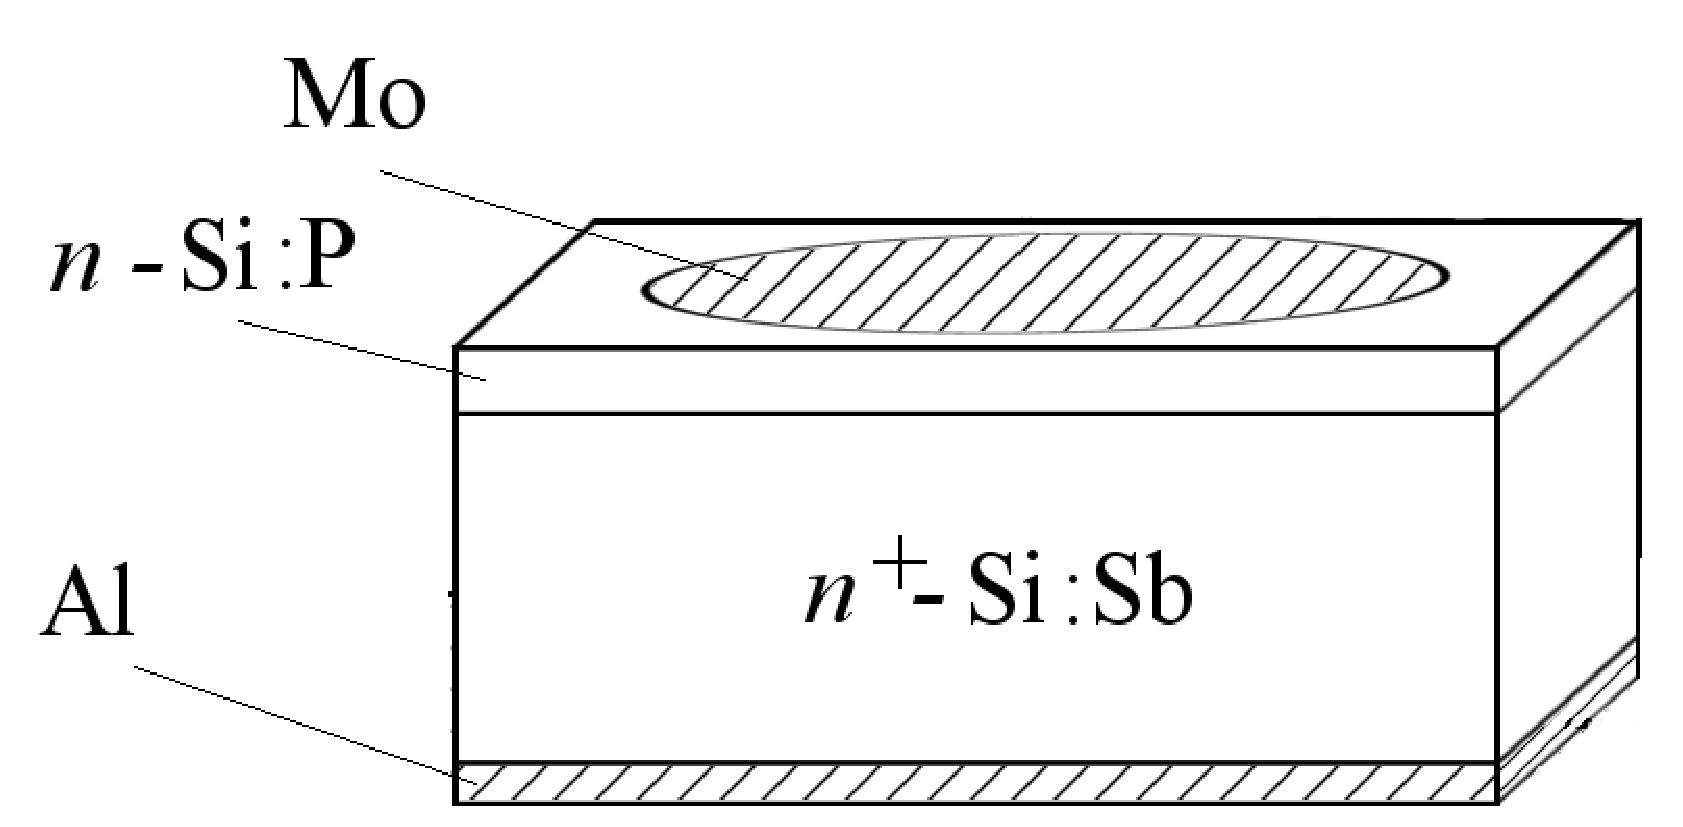
\includegraphics[width=0.65\textwidth]{MSSi}%
\caption{\label{figMSSi}
Структура зразків Mo$/n$--$n^+$--Si.
}
\end{figure}

В дослідженнях використовувалися структури МН (діоди Шотки (ДШ)), виготовлені на основі епітаксійної
структури $n$--$n^+$--Si.
Товщини епітаксійного шару та підкладки дорівнювали $0.2~\mu$м та $250~\mu$m, відповідно.
Епітаксійний шар був легований атомами фосфору, підкладка --- сурмою.
Для створення бар'єру на поверхню епітаксійного прошарку нанесено шар молібдену.
З протилежного боку структури нанесено прошарок алюмінію, який забезпечував наявність омічного контакту.
Схематичне зображення структур наведено на Рис.~\ref{figMSSi}.


В дисертації представлені результати, отримані з використанням кремнієвих ДШ двох типів,
які ідентичних за структурою, проте відрізняються концентраціями концентраціями носіїв заряду в епітаксійному шарі $N_d$ та
підкладці $N_s$, а також площею випрямляючого контакту $A$.
Для контролю рівня легування були виконані вимірювання вольт--фарадних характеристик (ВФХ) досліджуваних структур при кімнатній температурі ($T = 295$~К).
Параметри структур, а також їх позначення наведені в Таблиці~\ref{tabMSSi}.


\begin{table}
\caption{\label{tabMSSi}Параметри структур Mo$/n$--$n^+$--Si.
}
%\begin{tabular}{|c|c|c|c|}
\begin{tabularx}{\textwidth}{|>{\centering\arraybackslash}X|>{\centering\arraybackslash}X|>{\centering\arraybackslash}X|>{\centering\arraybackslash}X|>{\centering\arraybackslash}X|}
\hline
$N_d$, м$^{-3}$&$N_s$, м$^{-3}$&$A$, м$^2$&Позначення\\
\hline
$(1,1\div1,3)\cdot10^{23}$&$4,2\cdot10^{23}$&$3,14\cdot10^{-6}$&SSDA\\
\hline
$7,25\cdot10^{21}$&$4,2\cdot10^{22}$&$49\cdot10^{-6}$&SSDB\\
\hline
\end{tabularx}
\end{table}


\subsection{Cтруктури метал--напівпровідник на основі арсеніду галію}

\subsection{Кремнієві сонячні елементи}

\subsection{Монокристалічні структури арсеніду галію}

\subsection{Монокристали карбіду кремнію}

\section{Використання активного ультразвуку}


\section{Радіаційні обробки}
\subsection{Нейтронне опромінення}

\subsection{Опромінення $\gamma-$квантами}

\subsection{Мікрохвильове опромінення}



\chapter{Визначення параметрів структур метал--напівпровідник\label{Ch_MSMethod}}


\section{Загальні підходи до визначення параметрів діодів Шотки}
Напівпровідникові бар'єрні структури, як вже зазначалося раніше, надзвичайно широко застосовуються у техніці.
Параметри подібних структур є найбільш суттєвим фактором для можливості практичного використання,
а їх визначення відіграє надзвичайну важливу роль під час розробки, проектування та виготовлення пристроїв.
Одним з найпроширеніших шляхів визначення параметрів полягає у вимірюванні вольт--амперних характеристик (ВАХ).
В цьому випадку взаємозв'язок між струмом та напругою описується за допомогою певних фізичних моделей, в
результаті чого з'являється можливість вичленити параметри, спираючись на результати експериментальних вимірювань.
Наприклад, пряма гілка ВАХ ДШ згідно з моделлю термоемісії має описуватися \cite{Rhoderick1988} наступними виразами
\begin{eqnarray}
\label{eqSDIV}
I&=&I_s\left\{\exp\left[\frac{q(V-IR_s)}{n_\mathrm{id}kT}\right]-1\right\}\,,\\
\label{eqSDIs}
I_s&=&AA^*\,T^2\exp\left(-\frac{q\Phi_b}{kT}\right)\,,
\end{eqnarray}
де
$I_s$ --- струм насичення,
$q$ --- елементарний заряд,
$R_s$ --- послідовний опір,
$n_\mathrm{id}$ --- фактор неідеальності,
$k$ --- стала Больцмана,
$T$ --- абсолютна температура,
$A$ --- площа діоду,
$A^*$ --- ефективна стала Річардсона,
$\Phi_b$ --- висота бар'єру Шотки (ВБШ) при нульовому зміщенні.
$\Phi_b$ (або $I_s$), $n_\mathrm{id}$ та $R_s$ є найбільш фундаментальними параметрами даної моделі та повинні бути максимально точно визначені з експериментальних ВАХ.

В літературі запропоновано декілька методів визначення параметрів ДШ.
Найпростіший стандартний метод вимагає наявності лінійної області на залежності $\ln(I)$ від  $V$ \cite{Sze1985,Rhoderick1988}.
В цьому випадку два параметри, $n_\mathrm{id}$ та $\Phi_b$, можуть бути визначені за кутом нахилу та перетином  залежності з віссю струмів, відповідно.
На жаль, подібний підхід перестає бути дієздатним у випадку, коли структура характеризується значним послідовним опором.
Зокрема, рівняння~(\ref{eqSDIV}) перетворюється у трансцендентне, що суттєво ускладнює математичні аспекти визначення параметрів.
З одного боку, існує цілий набір аналітичних методів екстраполяції параметрів ДШ.
%Зважаючи на складність задачі, існує цілий ряд методів, які вирішують задачу екстраполяції параметрів ДШ.
Вони базуються на безпосередніх алгебраїчних наближеннях і використовують різноманітні допоміжні функції \cite{Norde,Lien,Werner,Cheung,Gromov,Lee,Bohlin,Cibils,Manifacier},
процедури  диференцювання  \cite{Mikhelashvili} або інтегрування  \cite{Kaminski,Ortiz1995,Durmus} ВАХ,
вимірювання ВАХ при декількох температурах \cite{Sato} або з використанням додаткового зовнішнього опору \cite{Lyakas}.

З іншого боку, визначення параметрів є багатовимірною задачею чисельної оптимізації і тому для її вирішення запропоновані різноманітні чисельні методи \cite{Ortiz1999,Evangelou,Donoval,Ferhat}.
Зазвичай, вони використовують метод найшвидшого градієнтного спуску для мінімізації різниці між виміряними та апроксимуючими значеннями.
При цьому деякі автори\cite{Lambert_Jung,Ortiz2005} шукають розв'язок рівняння~(\ref{eqSDIV}) використовуючи $W$--функцію Ламберта
\cite{LambertBook}.
Зазвичай, чисельні методи характеризуються більш високим рівнем достовірності визначення параметрів, проте нерідко вимагають відносно довгого часу для розрахунку.
Крім того, спостерігається тенденція збіжності у локальний екстремум замість глобального.

Нарешті, порівняно нещодавно було запропоновано використовувати еволюційні алгоритми (ЕА) для визначення параметрів напівпровідникових пристроїв \cite{PSO_Ye,DEWang,GA_Li,P-DE_Ishaque,TLBO_Patel,MABC,PSOWang,GA_Schottky}.
ЕА це стохастичний метод, який виявляє дуже високу ефективність при оптимізації дійсних цільових функцій багатьох змінних.
На відміну від чисельних методів, ЕА може бути застосований до нелінійних функцій без необхідності розрахунку похідних, а також слабко залежить від початкових наближень значень параметрів.
ЕА вважаються \cite{P-DE_Ishaque} найбільш багатообіцяючими  методами розрахунку параметрів.

У літературі наявні роботи \cite{Evangelou,Aubry,Kudryk}, в яких проводиться порівняння  та огляд шляхів визначення параметрів ДШ, проте вони переважно зосереджені на розгляді лише декількох метод і фактично не беруть до уваги еволюційні алгоритми.
Задача, яка вирішувалась під час досліджень, описаних у даному розділі, полягала у порівнянні ефективності (точності визначення параметрів та швидкості роботи) різних методів визначення параметрів МН--структур з ВАХ.
Крім того, розглянуте питання впливу величини окремих параметрів на точність визначення всього набору.
Було розглянуто підгрупу методів, які дозволяють визначити ВБШ, фактор неідеальності та послідовний опір використовуючи лише одну ВАХ.
Зокрема, увага сфокусована на 10 аналітичних методах, 2 чисельних методах та 4 еволюційних алгоритмах
(диференційної еволюції (DE, differential evolution),
оптимізації зграї частинок (PSO, particle swarm optimization),
модифікованої штучної бджолиної сім'ї (MABC, modified artificial bee colony) та
оптимізованого викладання та навчання (TLBO, teaching learning based optimization)).


Основні результати даного розділу представлені в роботах \cite{Olikh:Rev,6CPFCS}.

\section{Контрольні вольт--амперні характеристики}
Досліджені методи були застосовані до наборів ВАХ, отриманих як експериментально, так і синтезованих штучно.
В останньому випадку використовувалися як ідеальні характеристики, так і криві з певним рівнем шуму, який віддзеркалював можливість наявності випадкових похибок вимірювань у реальних умовах.

\subsection{Ідеальні синтезовані ВАХ}
Переважно, для оцінки спроможності визначення параметрів структур МН за допомогою аналітичних \cite{Norde,Lien,Werner,Gromov,Lee,Bohlin,Cibils,Mikhelashvili,Kaminski} та чисельних \cite{Evangelou,Donoval} методів, а також еволюційних алгоритмів \cite{PSO_Ye,P-DE_Ishaque,TLBO_Patel} використовують структури на основі кремнію.
Керуючись таким загальноприйнятим підходом, під час синтезу ВАХ вважалося, що використовуються кремнієвий ДШ.
ВАХ були розраховані за допомогою рівняння ~(\ref{eqSDIV}), для розв'язку якого застосовувався метод дихотомії.
При цьому використовувалися значення $A=3,14\cdot10^{-6}$~м$^2$ та $A^*=112$~A$\,$cм$^{-2}$K$^{-2}$ (випадок $n$--Si \cite{Schroder2006}).
Напруга змінювалась з кроком 0,01~В, струм вар'ювався в діапазоні $10^{-9}\div10^{-2}$~A.

Задача полягала у перевірці ефективності методів при різних значеннях параметрів і тому дані були синтезовані для діапазону температур від 130 до 330~К.
В той же час, ми намагались синтезувати ВАХ, які близькі до характеристик реальних діодів.
Тому температурні залежності $\Phi_b$, $n_\mathrm{id}$ та $R_s$ були обрані, спираючись на наступні міркування.
Як передбачено теорією \cite{Rhoderick1988} та спостережено на експерименті \cite{Aboelfotoh,Zhua},
для випадку однорідного контакту Шотки ВБШ має зменшуватись з підвищенням температури, причому очікувана залежність подібна до температурної залежності ширини забороненої зони напівпровідника.
Тому для апроксимації температурної залежності ВБШ використовувалося рівняння Варшні \cite{SiEg2012}
\begin{equation}
\label{eqFbT}
\Phi_b(T) = \Phi_b(0) - \frac{7.021\cdot10^{-4} T^2}{T + 1108} ,
\end{equation}
причому вважалося, що ВБШ при нульовій температури $\Phi_b(0)=0,75$~еВ.
Температурна залежність фактору неідеальності нерідко описується співвідношенням
\begin{equation}
\label{eqnT}
n_\mathrm{id}=1+\frac{T_0}{T},
\end{equation}
де величина константи $T_0$ для випадку кремнію знаходиться в діапазоні $20\div50$~K \cite{T0:Lee,T0:McCafferty,T0:Saxena,Aboelfotoh}.
Для синтезу ВАХ було використане значення $T_0=35$~K.
Температурна залежність послідовного опору може бути описана виразом \cite{Sze1985,Rs:Meyaard,Rs:Kang}
\begin{equation}
\label{eqRsT}
R_s=R_{s0}\exp\left(\frac{E_a}{kT}\right),
\end{equation}
де $E_a$ -- енергія активації легуючої домішки.
В роботі були використані значення $E_a=0,044$~еВ (що відповідає домішковому атому фосфору) та $R_{s0}=0.25$~Ом.

Як наслідок, набір синтезованих для аналізу ВАХ складався з 21 кривої, які відповідали інтервалу температуз $130\div330$~К з кроком 10~К.
При цьому  $\Phi_b$, $n_\mathrm{id}$ змінювались $R_s$ від 0,740 до 0,697~еВ, від 1,27 до 1,11 та від 12,6 to 1,2~Ом, відповідно.


\subsection{Синтезовані ВАХ з випадковими похибками}
Для того, щоб моделювати можливі випадкові похибки, які виникають під час вимірювань, та проаналізувати стійкість методів визначення параметрів до їх наявності,
були також синтезовані набори ВАХ, в яких значення напруги та струму вибиралися з певним рівнем шуму.
В цьому випадку напруга $V_i$ та струм $I_i$, які відповідали $i-$й точці ВАХ вибиралися випадковим чином використовуючи розподіл Гауса.
Тобто, густина ймовірності очікування певної величини напруги описувалася виразом
\begin{equation}
\label{eqGaus}
f(V_i,\overline{V}_i,\sigma_V)=\frac{1}{\sigma_V\sqrt{2\pi}}\exp\left[-\frac{(V_i-\overline{V}_i)^2}{2\sigma_V^2}\right].
\end{equation}
При цьому середнє значення (сподівання) напруги $\overline{V}_i$ змінювалося з кроком 0,01~В,
середнє значення сили струму $\overline{I}_i$ обчислювалося використовуючи рівняння~(\ref{eqSDIV}) та $\overline{V}_i$.
Стандартне відхилення (дисперсія) напруги $\sigma_V$ вибиралася сталою для всього набору (21 криві) ВАХ.
Стандартне відхилення сили струму $\sigma_I$ залежало від величини сили струму $\sigma_I=\sigma_I^\varepsilon\cdot\overline{I}_i$,
де постійна для набору ВАХ величина $\sigma_I^\varepsilon$ --- відносна дисперсія струму.
Такий підхід відповідає достатньо поширеному на практиці випадку, коли відносні похибки вимірювання напруги та струму залишаються сталими для всієї ВАХ.
Надалі для позначення синтезованих подібним чином ВАХ буде використовуватися термін "зашумлені синтезовані дані" (noisy synthetic data).

Різні набори синтезованих ВАХ відрізнялися значеннями $\sigma_V$ та $\sigma_I^\varepsilon$.
Фактично, для ідеальних синтезованих ВАХ $\sigma_V=0$~В and $\sigma_I^\varepsilon=0$.


\subsection{Експериментальні ВАХ}
Досліджені методи були застосовані також до експериментально виміряних ВАХ кремнієвих структур SSDA, описаних в параграфі~\ref{MSSi}.
Параметри ДШ визначались на основі характеристик, отриманих в інтервалі температур $130\div330$~К, який співпадав з діапазоном синтезованих ВАХ.

\section{Критерії точності методів}
У випадку, коли методи застосовувалися для аналізу синтезованих ВАХ, проводилося оцінювання точності визначення параметрів.
Зокрема, для кількісної оцінки точності кожного з методів використовувалися наступні величини.
Наприклад, оцінювання визначення фактору неідеальності з однієї ВАХ $\chi^q_n$ здійснювалося за допомогою виразу
\begin{equation}
\label{eqniac}
\chi^q_n=\left(\frac{n_{\mathrm{id},ext}-n_{\mathrm{id},ac}}{n_{\mathrm{id},ac}}\right)^2,
\end{equation}
де
$n_{\mathrm{id},ext}$ --- значення, отримане в результаті застосування методу,
$n_{\mathrm{id},ac}$ --- точне значення, яке використовувалося під час синтезу ВАХ.


Точність визначення $n_\mathrm{id}$ на всьому наборі ВАХ $\varepsilon_n$ обчислювалася  наступним чином:
\begin{equation}
\label{eqnac}
\varepsilon_n=\sqrt[2N_{I\!V}]{\prod_{i=1}^{N_{I\!V}}\chi^q_{n,i}},
\end{equation}
де
$N_{I\!V}$ --- загальна кількість ВАХ у наборі.
Зауважимо, що $\varepsilon_n$ --- це квадратних корінь з середньо-геометричного значення $\chi^q_n$.
Для оцінювання точності визначення ВБШ та послідовного опору з однієї ВАХ використовувалися величини  $\chi^q_\Phi$ та $\chi^q_R$, а для набору ВАХ --- $\varepsilon_\Phi$ and $\varepsilon_R$, для розрахунку яких використовувалися вирази, аналогічні (\ref{eqniac}) та (\ref{eqnac}), відповідно.

\section{Короткий огляд використаних методів}
\subsection{Аналітичні методи}
Модифікований метод Норда \cite{Norde,Lien,Sato,Dermircioglu:Norde} базується на використанні допоміжної функції
\begin{equation}
\label{eqNorde}
F(V)=\frac{V}{\gamma_N}-\frac{kT}{q}\ln\left(\frac{I(V)}{AA^*T^2}\right),
\end{equation}
де
$\gamma_N$ --- довільна константа, яка має бути більша, ніж фактор неідеальності.
При цьому величини ВБШ та послідовного опору визначаються за допомогою співвідношень
\begin{eqnarray}
\label{eqNordDet}
\Phi_b&=&F(V_{min})+\frac{\gamma_N-n_\mathrm{id}}{n_\mathrm{id}}\left(\frac{V_{min}}{\gamma_N}-\frac{kT}{q}\right),
\\
R_s&=&\frac{(\gamma_N-n_\mathrm{id})kT}{qI_{min}}\,,
\end{eqnarray}
де
$F(V_{min})$ та $V_{min}$ --- це координати точки мінімуму залежності $F(V)$ від $V$;
$I_{min}$  --- струм, який на ВАХ відповідає $V_{min}$.

Необхідно підкреслити, що згідно з цим методом, значення $n_\mathrm{id}$ має бути відомим.
Як наслідок, при застосування метода Норда до синтезованих та експериментальних ВАХ, використовувалися величини $n_{\mathrm{id},ac}$ та значення, отримане з використанням методу MABC, відповідно.

Крім того, для випадку  $R_s<5$~Ом, мінімум функції Норда $F(V)$, побудованої на основі ВАХ в діапазоні струмів до $10^{-2}$~А, не спостерігався взагалі.
Тому при застосуванні цього методу, так і методу Бохліна (описаного нижче), використовувалися набори ВАХ, синтезовані в більш широкому струмовому діапазоні, від $10^{-9}$ до $10^{-2}$~A.

Нарешті, проведені розрахунки показали, що точність методу Норда залежить від вибраної величини $\gamma_N$.
Відповідні залежності наведено на Рис.~\ref{figNorde}.
Зокрема показано, що похибка визначення $\Phi_b$ збільшується зі зростанням $\gamma_N$ як для випадку ідеальних синтезованих ВАХ, так і при використанні зашумлених даних.
В той же час, похибка визначення  $R_s$
а)~зменшується зі зростанням $\gamma_N$ при $\gamma_N<2$ і залишається сталою при $\gamma_N>2,5$ для зашумлених даних;
б)~немонотонно залежить від $\gamma_N$ для ідеальних синтезованих ВАХ.
Враховуючи виявлені суперечливі тенденції для мінімізації похибки методу Норда при отриманні наведених надалі даних використовувалося значення $\gamma_N=1,8$.

Для позначення результатів, отриманих з використанням методу Норда, використовується мітка <<Norde>>.

\begin{figure}
\center
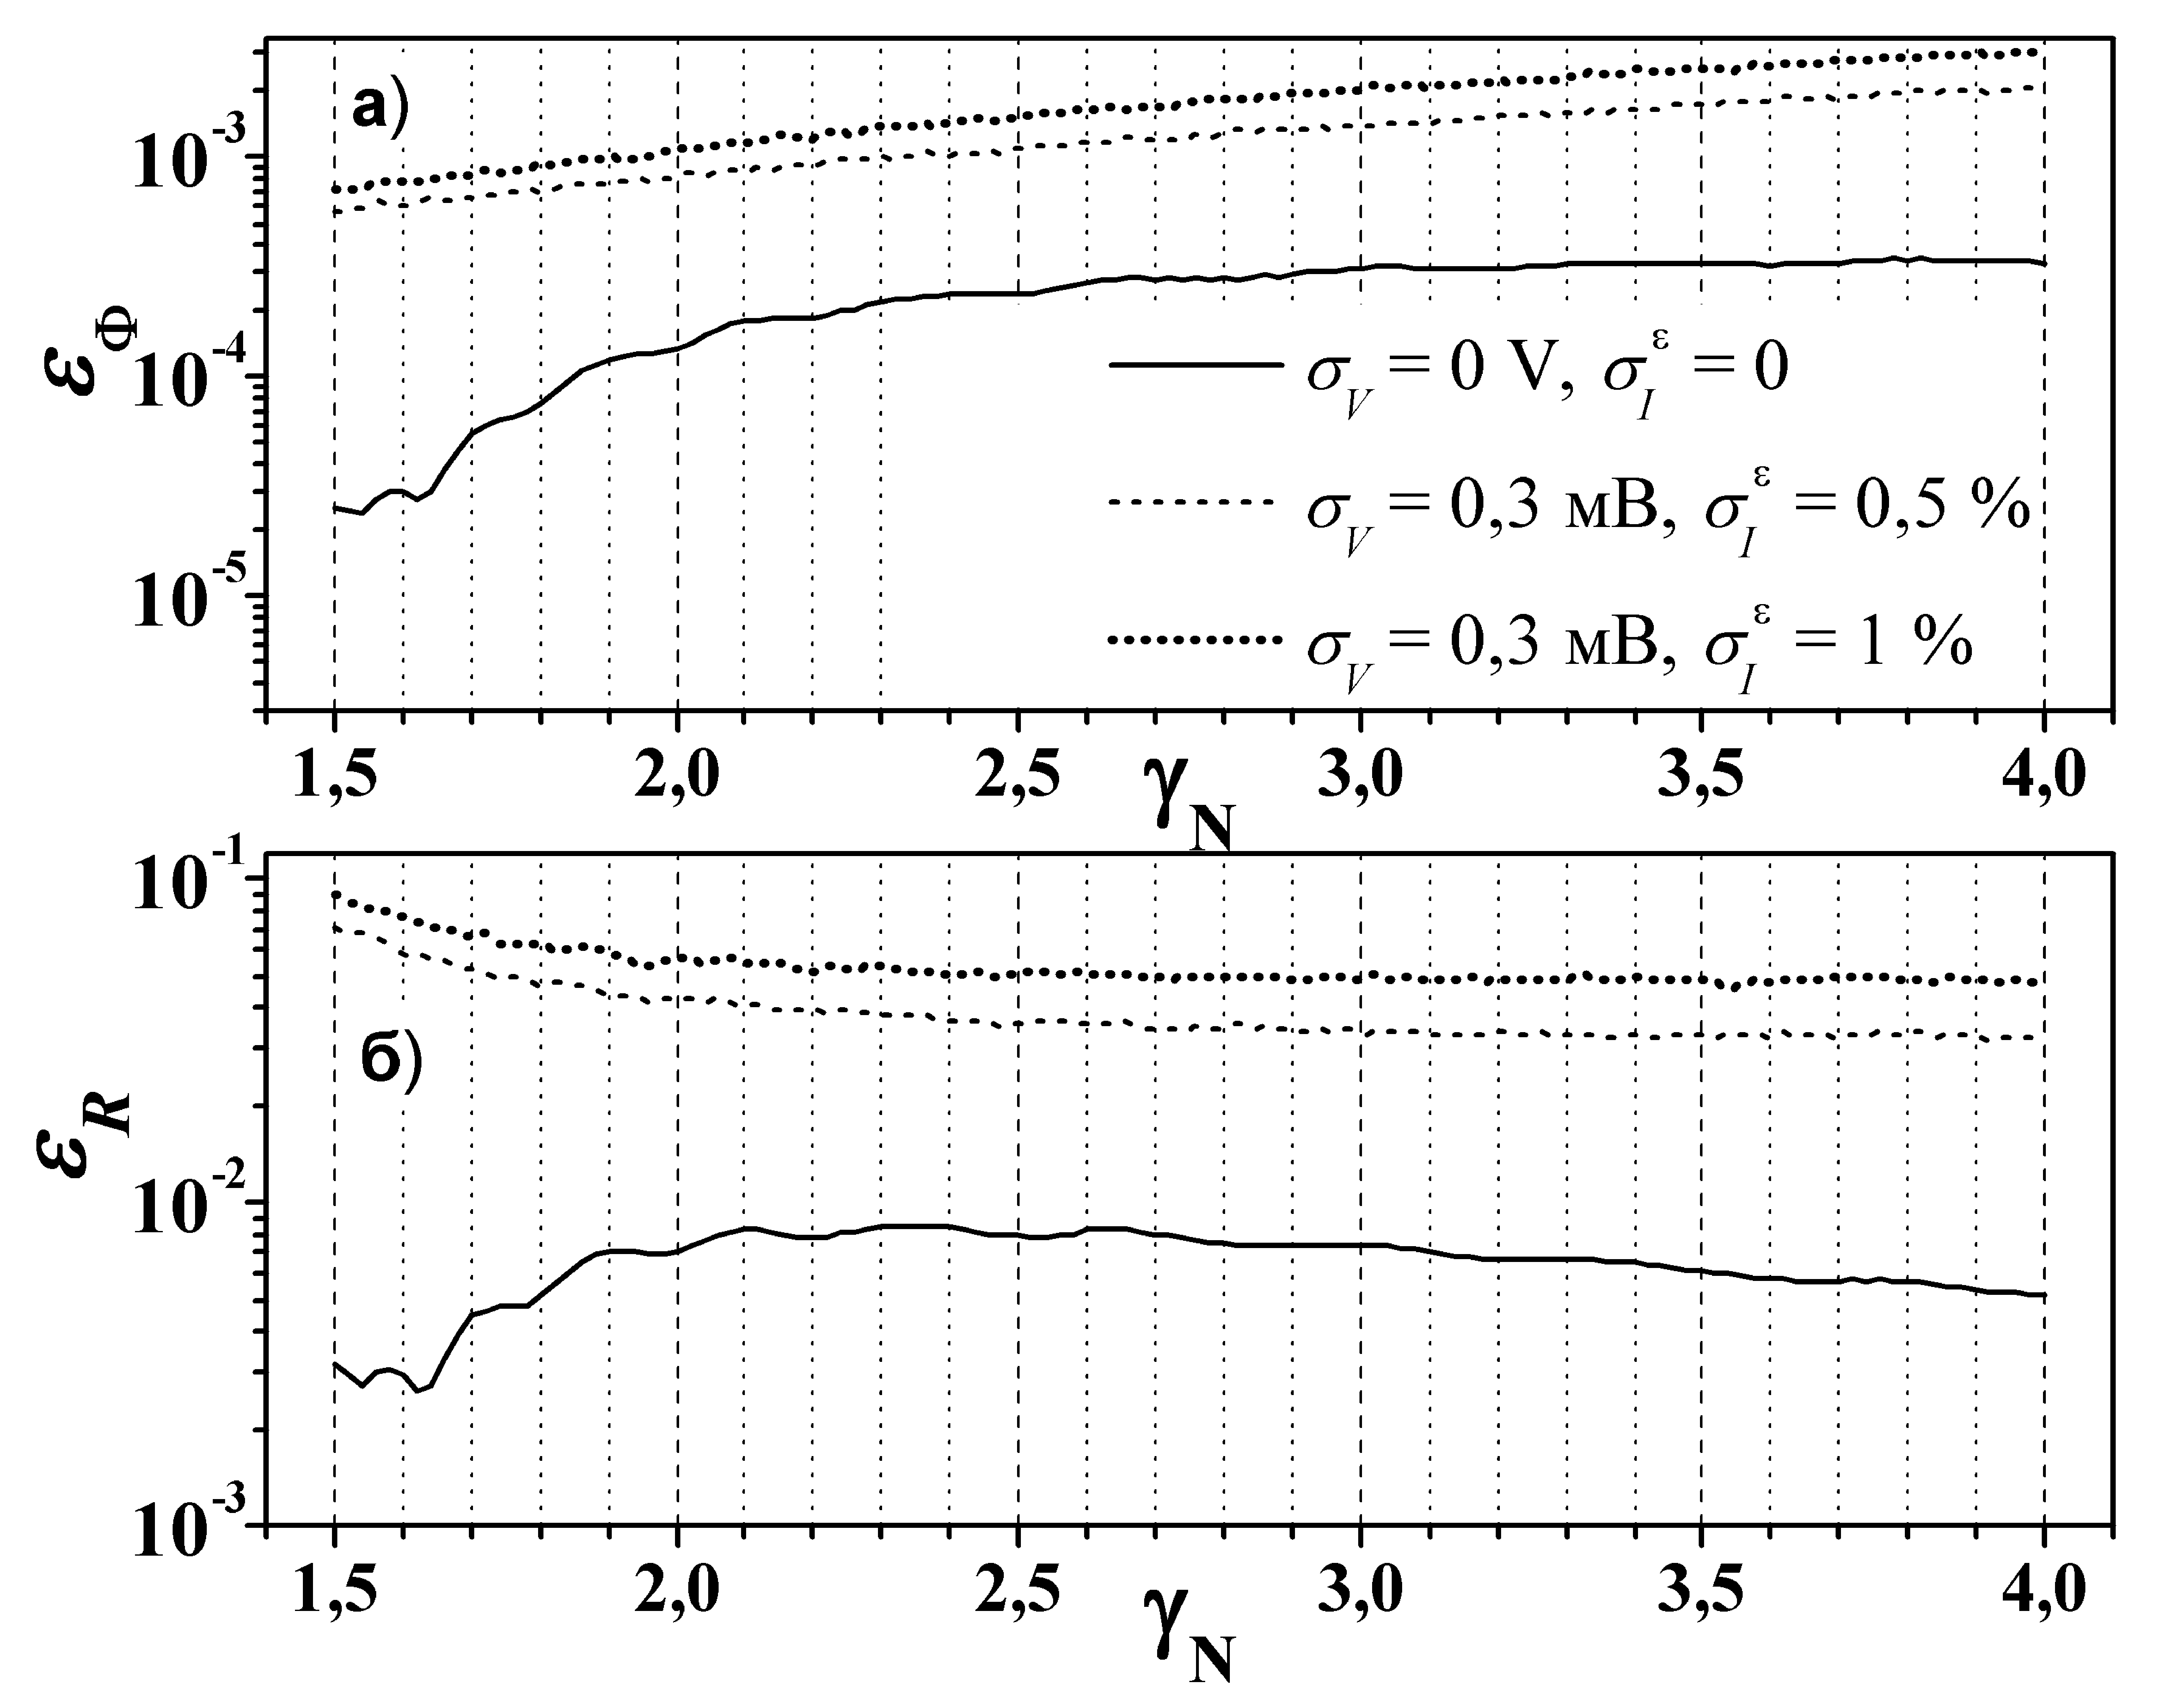
\includegraphics[width=0.8\textwidth]{figNorde}%
\caption{\label{figNorde}
Залежності точності визначення $\Phi_b$ (a) та $R_s$ (б)  від величини $\gamma_N$.
 при застосуванні метода Норда до набору ідеальних синтезованих ВАХ (суцільні лінії) та зашумлених даних (штрихові лінії).
}
\end{figure}

J.~Werner  \cite{Werner} показав, що за умови коли падіння напруги в області бар'ру $V_d=(V-IR_s)\gg nkT/q$, то
\begin{equation}
\label{eqWerner}
\frac{(dI/dV)}{I}=\frac{q}{nkT}\left[1-R_s\left(\frac{dI}{dV}\right)\right].
\end{equation}
Рівняння~(\ref{eqWerner}) показує, що графік  залежності   $(dI/dV)/I$  від $(dI/dV)$ має бути прямою лінією,
причому її нахил та точка перетину з вертикальною віссю визначаються $R_s$ and $n_\mathrm{id}$.

На жаль, даний метод дозволяє визначити лише два параметри ДШ.
Для оцінки величини ВБШ була використана наступна процедура.
Спираючись на визначене значення $R_s$, експериментальна або синтезована ВАХ корелювалася і проводилась побудова залежності  $\ln I$ від $V_d$.
Після цього проводилась апроксимація отриманої залежності лінійною функцією за методом найменших квадратів в діапазоні $V_d>3kT/q$.
Необхідно підкреслити, що під час апроксимації нахил кривої може розглядатися або як незалежна величина, яка обчислюється, або як відома величина, що визначається попередньо визначеним (під час апроксимації функції (eqWerner)) значенням $n_\mathrm{id}$.
В роботі розглянуто обидва випадки.
Якщо величини $R_s$ and $n_\mathrm{id}$ визначались шляхом лінійної апроксимації функції (eqWerner), а $\Phi_b$ --- як перетин залежності $\ln I=f(V_d)$ при відомому нахилі, то використовується позначення <<Werner>>.
Якщо ж лише $R_s$ визначається за допомогою функції Вернера (\ref{eqWerner}), а $\Phi_b$ and $n_\mathrm{id}$ обчислюються потім із залежності $\ln I=f(V_d)$, то використовується позначення <<Werner*>>.
Подібний підхід до позначень отриманих результатів (із зірочкою та без неї належно від того, скільки незалежних величин використовується при апроксимації скорельованих відповідно до визначеного раніше значення послідовного опору ВАХ) використовуються і для інших методів, детальніше описаних нижче.

R.~Cibils  та R.~Buitrago \cite{Cibils} запропонували використовувати допоміжну функцію у вигляді
\begin{equation}
\label{eqCibils}
F_a(V)=V-V_a\ln I,
\end{equation}
де
$V_a$ практично довільне значення напруги, $V_a\geq99,5I_sR_s+n_\mathrm{id}kT/q$.
Якщо $I_{min,a}$ --- це значення струму, яке відповідає напрузі $V_{min}$, при якій спостерігається мінімум функції $F_a(V)$,
то залежність $I_{min,a}$ від $V_a$ має бути \cite{Cibils} лінійною:
\begin{equation}
\label{eqCibilsDet}
I_{min,a}=(V_a-n_\mathrm{id}kT/q)/R_s\,.
\end{equation}
В роботі при побудові сімейства допоміжних функцій згідно з виразом (\ref{eqCibils}), використовувалися значення  $V_a$ в діапазоні від 0,035~В до максимального значення напруги для даної ВАХ.
Крок зміни $V_a$ дорівнював 1~мВ.
Отримані результати позначені міткою <<Cibils>>.

А.~Kaminski зі співавторами \cite{Kaminski} запропонували два методи.
Перший з них використовує допоміжну функцію, яка будується з використанням інтегрування ВАХ.
Так, ордината та абсциса $j-$ої точки допоміжного графіку розраховуюся як
\begin{equation}
\label{eqKam1}
Y_j=\frac{1}{I_j-I_1}\int_{V_1}^{V_j}I\,dV \quad\text{and}\quad X_j=\frac{I_j+I_1}{2},
\end{equation}
де
$V_i$ та $I_i$ --- це координати $i-$ої точки ВАХ,
$i\in(1,\ldots, N_p)$,
$j\in(2,\ldots, N_p)$.
Згідно з цим методом очікується, що залежність $Y$ від $X$ має бути лінійною, причому
\begin{equation}
\label{eqKam1Det}
Y=n_\mathrm{id}kT/q+R_sX.
\end{equation}
Тобто, лінійна апроксимація допоміжної функції дозволяє визначити $R_s$ та $n_\mathrm{id}$.

В роботі лінійна апроксимація здійснювалась за допомогою методу найменших квадратів.
Чисельне інтегрування ВАХ здійснювалось за методом трапецій.
Отримані результаті позначені мітками <<Kaminski I>> та <<Kaminski* I>>.

У другому методі, розглянутому в роботі \cite{Kaminski}, також використовується допоміжна функція $Y$ від $X$, проте
\begin{equation}
\label{eqKam2}
Y_k=\frac{\ln(I_j/I_i)}{I_j-I_i} \quad\text{and}\quad X_k=\frac{V_j-V_i}{I_j-I_i},
\end{equation}
$i\in(1,\ldots, N_p-1)$,
$j\in(i+1,\ldots, N_p)$,
$k\in(1,\ldots, N_p(N_p-1)/2)$.
Отримана таким чином залежність має бути прямолінійною:
\begin{equation}
\label{eqKam2Det}
Y=q(-R_s+X)/n_\mathrm{id}kT.
\end{equation}
Отримані за допомогою даного підходу результати позначені мітками <<Kaminski II>> та <<Kaminski* II>>.

У методі, запропонованому в роботі \cite{Bohlin}, використовуються дві функції Норда, побудовані з використанням двох різних значень $\gamma_N$:
\begin{eqnarray}
\label{eqBohlin}
F_1(V)&=&V/\gamma_1-kT/q\cdot\ln(I/AA^*T^2),
\nonumber\\
F_2(V)&=&V/\gamma_2-kT/q\cdot\ln(I/AA^*T^2).
\end{eqnarray}
Передбачено, що параметри ДШ визначаються за допомогою співвідношень
\begin{eqnarray}
\label{eqBohlinDet}
n_\mathrm{id}&=&\frac{1}{2}\left[\frac{\gamma_1I_{min,2}-\gamma_2I_{min,1}}{I_{min,2}-I_{min,1}}+\right.
\\
&&\left.\frac{V_{min,1}-V_{min,2}+(\gamma_2-\gamma_1)kT/q}{F_2(V_{min,2})-F_1(V_{min,1})-V_{min,2}/\gamma_2+V_{min,1}/\gamma_1}\right]
,\nonumber
\\
Rs&=&\frac{kT}{2q}\left[\frac{\gamma_1-n_\mathrm{id}}{I_{min,1}}+\frac{\gamma_2-n_\mathrm{id}}{I_{min,2}}\right]\,,
\\
\Phi_b&=&\frac{1}{2}\left[F_1(V_{min,1})+\frac{(\gamma_1-n_\mathrm{id})(qV_{min,1}-\gamma_1kT)}{\gamma_1qn_\mathrm{id}}\,+\right.
\nonumber\\
&&\left.F_2(V_{min,2})+\frac{(\gamma_2-n_\mathrm{id})(qV_{min,2}-\gamma_2kT)}{\gamma_2qn_\mathrm{id}}\right].
\end{eqnarray}
де
$[F_1(V_{min,1}), V_{min,1}]$ та $[F_2(V_{min,2}), V_{min,2}]$ --- це координати мінімумів функцій  $F_1(V)$ від $V$ та $F_2(V)$ від $V$, відповідно;
$I_{min,1}$ та $I_{min,2}$ --- значення струму, які відповідають на ВАХ значенням напруги $V_{min,1}$ та $V_{min,2}$, відповідно.

Проведені чисельні дослідження показали, що, як і в методі Норда, в цьому випадку точність визначення параметрів залежить від вибору величин $\gamma_1$ та $\gamma_2$.
Отримані результати приведені на Рис.~\ref{figBohlin}.
Зокрема виявлено, що похибка екстрагування параметрів зростає при збільшенні модуля різниці параметрів $|\gamma_1-\gamma_2|$.
З метою мінімізації помилок методу в подальшому наведені результати, отримані при використанні величин $\gamma_1=1,6$ та $\gamma_2=3,5$.
Отримані результати позначені міткою <<Bohlin>>.

\begin{figure}
\center
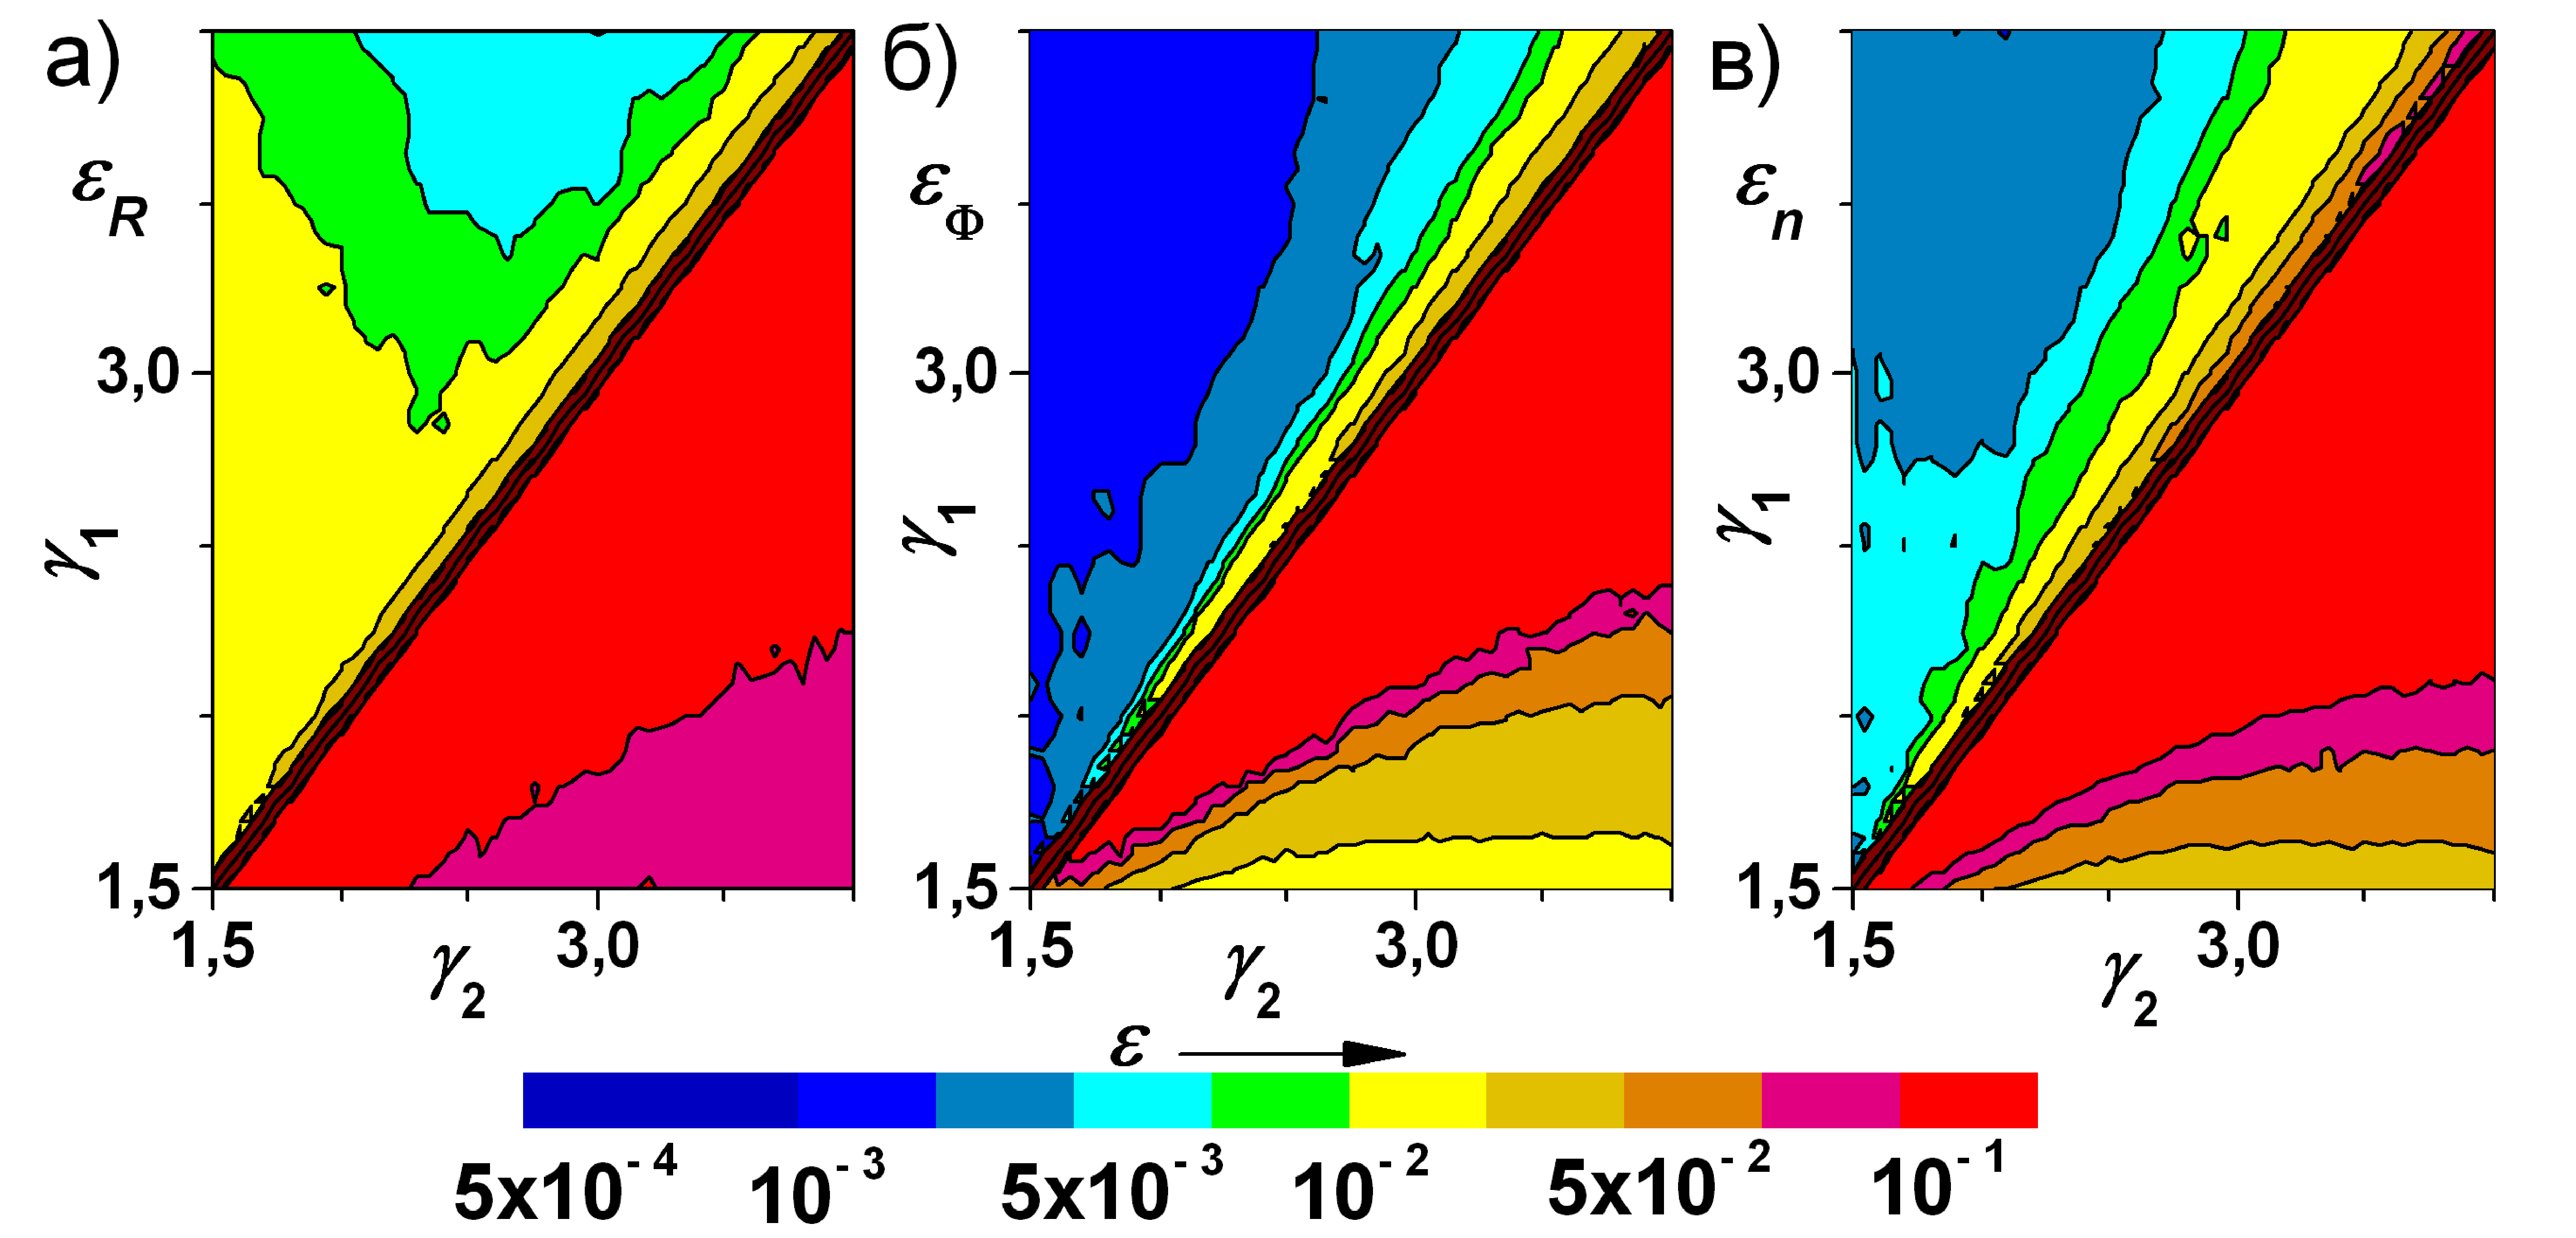
\includegraphics[width=1\textwidth]{figBohlin}%
\caption{\label{figBohlin}
Залежності точностей визначення $R_s$ (a), $\Phi_b$ (б) та $n_\mathrm{id}$ (в) від величини параметрів $\gamma_1$ та $\gamma_2$ при застосуванні метода Бохліна.
Наведено результати, отримані для наборів ідеальних ($\sigma_V=0$~V, $\sigma_I^\varepsilon=0$) синтезованих ВАХ (область $\gamma_1>\gamma_2$) та зашумлених ($\sigma_V=0,3$~мВ, $\sigma_I^\varepsilon=1\%$) даних (область $\gamma_2>\gamma_1$).
}
\end{figure}

В роботі \cite{Lee} для визначення параметрів ДШ запропоновано використовувати масив функцій $\{F_L(I)\}$:
\begin{equation}
\label{eqLee}
F_L(I)=V(I)-V_a\ln I,
\end{equation}
де
$V_a$ --- це довільне значення напруги.
Кожна з функцій $F_L(I)$ має бути апроксимована залежністю
\begin{equation}
\label{eqGrFit}
y(I)=c_1+c_2I+c_3\ln I
\end{equation}
та параметри $c_1$, $c_2$ та $c_3$ мають бути визначені.
Тоді очікується \cite{Lee}, що при $V>3kT/q$,
залежність $I_a=-c_3/c_2$ від $V_a$ має бути лінійною:
\begin{equation}
\label{eqLeeDet}
I_a(V_a)=(-n_\mathrm{id}kT/q+V_a)/R_s,
\end{equation}
що дозволяє визначити послідовний опір та фактор неідеальності.
В свою чергу, $\Phi_b$ може бути розрахований \cite{Lee} за допомогою виразу
\begin{equation}
\label{eqLeeFb}
\Phi_b=c_3/n_\mathrm{id}+kT/q\cdot\ln\left(AA^*T^2\right).
\end{equation}

В роботі при застосуванні даного методу використовувалися значення $V_a$ починаючи з 40~мВ з кроком 20~мВ;
апроксимація $F_L(I)$ здійснювалась за методом найменших квадратів.
Отримані дані позначені міткою <<Lee>>.

В роботі Д.~Громова та В.~Пугачевича \cite{Gromov} розглянуто два можливі шляхи визначення параметрів ДШ.
Згідно з першим з них, залежність напруги від струму може бути апроксимована виразом (\ref{eqGrFit}) причому
\begin{eqnarray}
\label{eqGr1}
R_s&=&c_2\,,
\\
n_\mathrm{id}&=&(c_3q)/(kT)\,,
\\
\Phi_b&=&\left[c_1/c_3+\ln\left(AA^*T^2\right)\right]kT/q\,.
\end{eqnarray}
Другий шлях полягає у тому, що вираз (\ref{eqGrFit}) застосовується до апроксимації функції Норда з $\gamma_N=2$:
\begin{equation}
\label{eqGr2}
F(I)=V(I)/2-kT/q\cdot\ln(I/AA^*T^2).
\end{equation}
В цьому випадку \cite{Gromov}
\begin{eqnarray}
\label{eqGr2Det}
R_s&=&2c_2\,,
\\
n_\mathrm{id}&=&(2c_3q)/(kT)+2\,,
\\
\Phi_b&=&\frac{2c_1}{n_\mathrm{id}}+\frac{(2-n_\mathrm{id})kT}{n_\mathrm{id}q}\ln\left(AA^*T^2\right)\,.
\end{eqnarray}
Застосування методів показало, що обидва підходи приводять до абсолютно однакових результатів.
Більше того, визначені значення параметрів дуже близькі до даних, які отримані за однакових початкових умов при використанні методу, описаного в роботі \cite{Lee} та згаданого трохи вище.
Тобто ці методи не є незалежними.

З іншого боку, проведені оцінки показали, що точність визначення параметрів за допомогою цих методів залежить від діапазону вихідної ВАХ, який використовується для побудови допоміжної функції, яка потім апроксимується залежністю (\ref{eqGrFit}).
Так, на Рис.~\ref{figGromov} наведено залежності похибок екстрагованих параметрів від початкового значення діапазону напруг, в якому проводилась апроксимація.
Видно, що для ідеальних ВАХ точність підвищується при звуженні використаного діапазону.
Водночас, для зашумлених даних спостерігається екстремальне значення точності  при певних значеннях ширини діапазону.
Причому ширина та положення діапазону, при якому точність визначення параметрів найбільша, залежить від рівня шуму.



\begin{figure}
\center
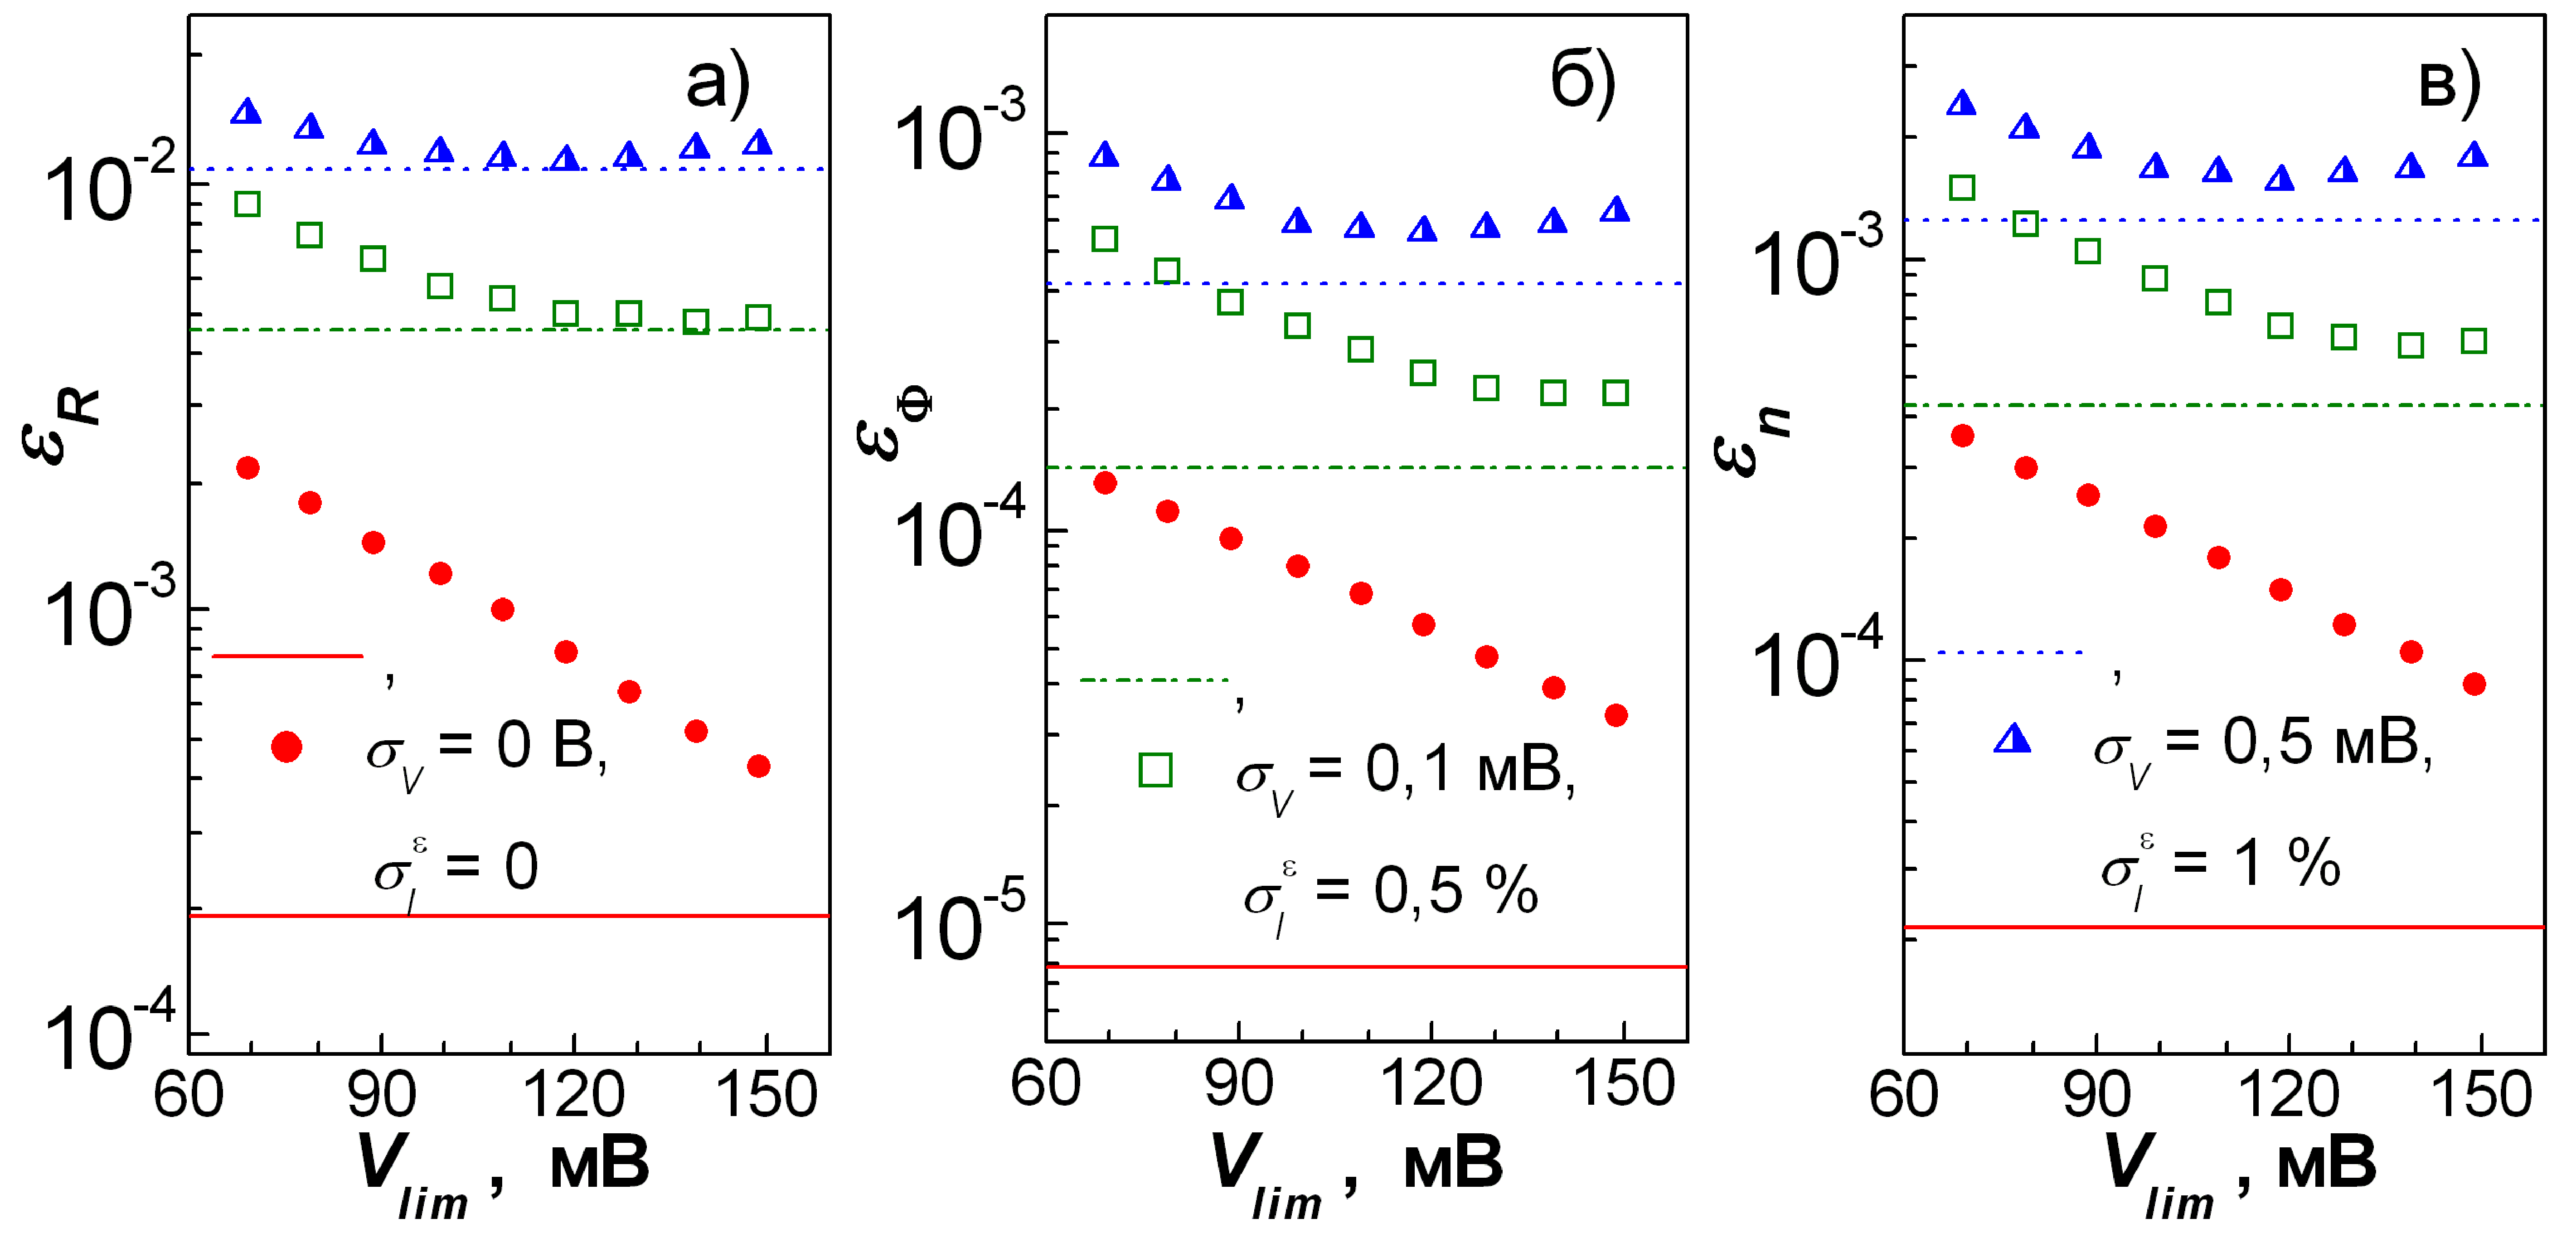
\includegraphics[width=1\textwidth]{figGromov}%
\caption{\label{figGromov}
Залежності точності визначення $R_s$ (a), $\Phi_b$ (б) та $n_\mathrm{id}$ (в) при використанні методу Громова.
Наведено результати, отримані при апроксимуванні залежністю (\ref{eqGrFit}) допоміжної функції, побудованої
на основі ділянки ВАХ в діапазоні напруг від $V_{lim}$ до максимально значення.
Горизонтальні лінії вказують похибки значень параметрів ДШ, які отримані при використанні адаптивної процедури (див. текст).
Представлені результати, отримані при застосуванні методу до ідеальних синтезованих ВАХ (заповнені кружечки, суцільні лінії) та зашумлених даних
з $\sigma_V=0,1$~мВ та $\sigma_I^\varepsilon=0,5\%$ (незаповлені квадрати, штрих--пунктирні лінії) та з $\sigma_V=0,5$~мВ та $\sigma_I^\varepsilon=1\%$
(напівзаповнені трикутники, пунктирні лінії)
}
\end{figure}

У зв'язку з цим, для покращення ефективності роботи методів Громова та Лі, пропонується використовувати спеціальну адаптивну процедуру вибору діапазону побудови допоміжної функції.
Вона полягає в тому, що параметрів визначаються для всіх можливих діапазонів, кількість яких залежить від кількості точок вихідної ВАХ.
Після цього для кожного отриманого набору параметрів обчислюється величина $\theta=\sum_{i=1}^{N_p}[1-I_{calc}(V_i)/I_i]^2$,
де $I_{calc}(V_i)$ розраховується з використанням виразів (\ref{eqSDIV}) та (\ref{eqSDIs}).
Найкращим за точністю вважається той набір параметрів, для якого спостерігається мінімум величини $\theta$.

Зрозуміло, що подібна адаптивна процедура збільшує час, необхідних для визначення параметрів ДШ через необхідність багатократного повторення застосування методу Громова (Лі) та додаткових розрахунків.
Проте, з іншого боку, ця процедура може бути автоматизована, а також дозволяє підвищити точність --- див. лінії на Рис.~\ref{figGromov}.

Нижче представлені результати застосування методу Громова з використанням запропонованої адаптивної процедури.
Отримані дані позначені міткою <<Gromov>>.
Різниця між ними та позначеними міткою <<Lee>> визначає, фактично, доцільність запропонованої процедури.

В роботі \cite{Cheung} запропоновано визначати параметри ДШ шляхом побудови залежностей функцій $H(V)$
\begin{equation}
\label{eqH}
H(I)=V-\frac{n_\mathrm{id}kT}{q}\ln\left(\frac{I}{AA^*T^2}\right).
\end{equation}
та $dV/d(\ln I)$ від сили струму.
За умови $V_d>3kT/q$ ці залежності мають бути лінійними, причому
\begin{eqnarray}
\label{eqChung}
\frac{dV}{d\ln I}&=&R_sI+n_\mathrm{id}kT/q,
\\
\label{eqHDet}
H(I)&=&n_\mathrm{id}\Phi_b+IR_s.
\end{eqnarray}
При застосуванні методу спочатку визначаються $R_s$ та  $n_\mathrm{id}$ на основі рівняння (\ref{eqChung}),
а потім  $\Phi_b$, використовуючи вираз~(\ref{eqHDet}) та обчислене на попередньому кроці значення $n_\mathrm{id}$.
Отримані результати позначені міткою <<Chung>>.

Ще одним методом, де використовуються диференційні коефіцієнти ВАХ, є запропонований в роботі \cite{Mikhelashvili}.
В цьому випадку все починається з обчислення функції  $\alpha(V)$:
\begin{equation}
\label{eqMikh}
\alpha(V)=d(\ln I)/d(\ln V).
\end{equation}
Визначення параметрів відбувається з використанням співвідношень
\begin{eqnarray}
\label{eqMikhDet}
R_s&=&\frac{V_{max}}{\alpha^2_{max}I_{max}}\,,
\\
n_\mathrm{id}&=&\frac{qV_{max}(\alpha_{max}-1)}{\alpha_{max}^2kT}\,,
\\
\Phi_b&=&\frac{kT}{q}\left[\alpha_{max}+1-\ln\left(\frac{I_{max}}{AA^*T^2}\right)\right]\,.\label{eqMikhDetFi}
\end{eqnarray}
де
$\alpha_{max}$ та $V_{max}$  це координати максимуму залежності $\alpha$ від $V$;
$I_{max}$ --- сила струму, яка відповідає напрузі $V_{max}$.

\begin{figure}
\center
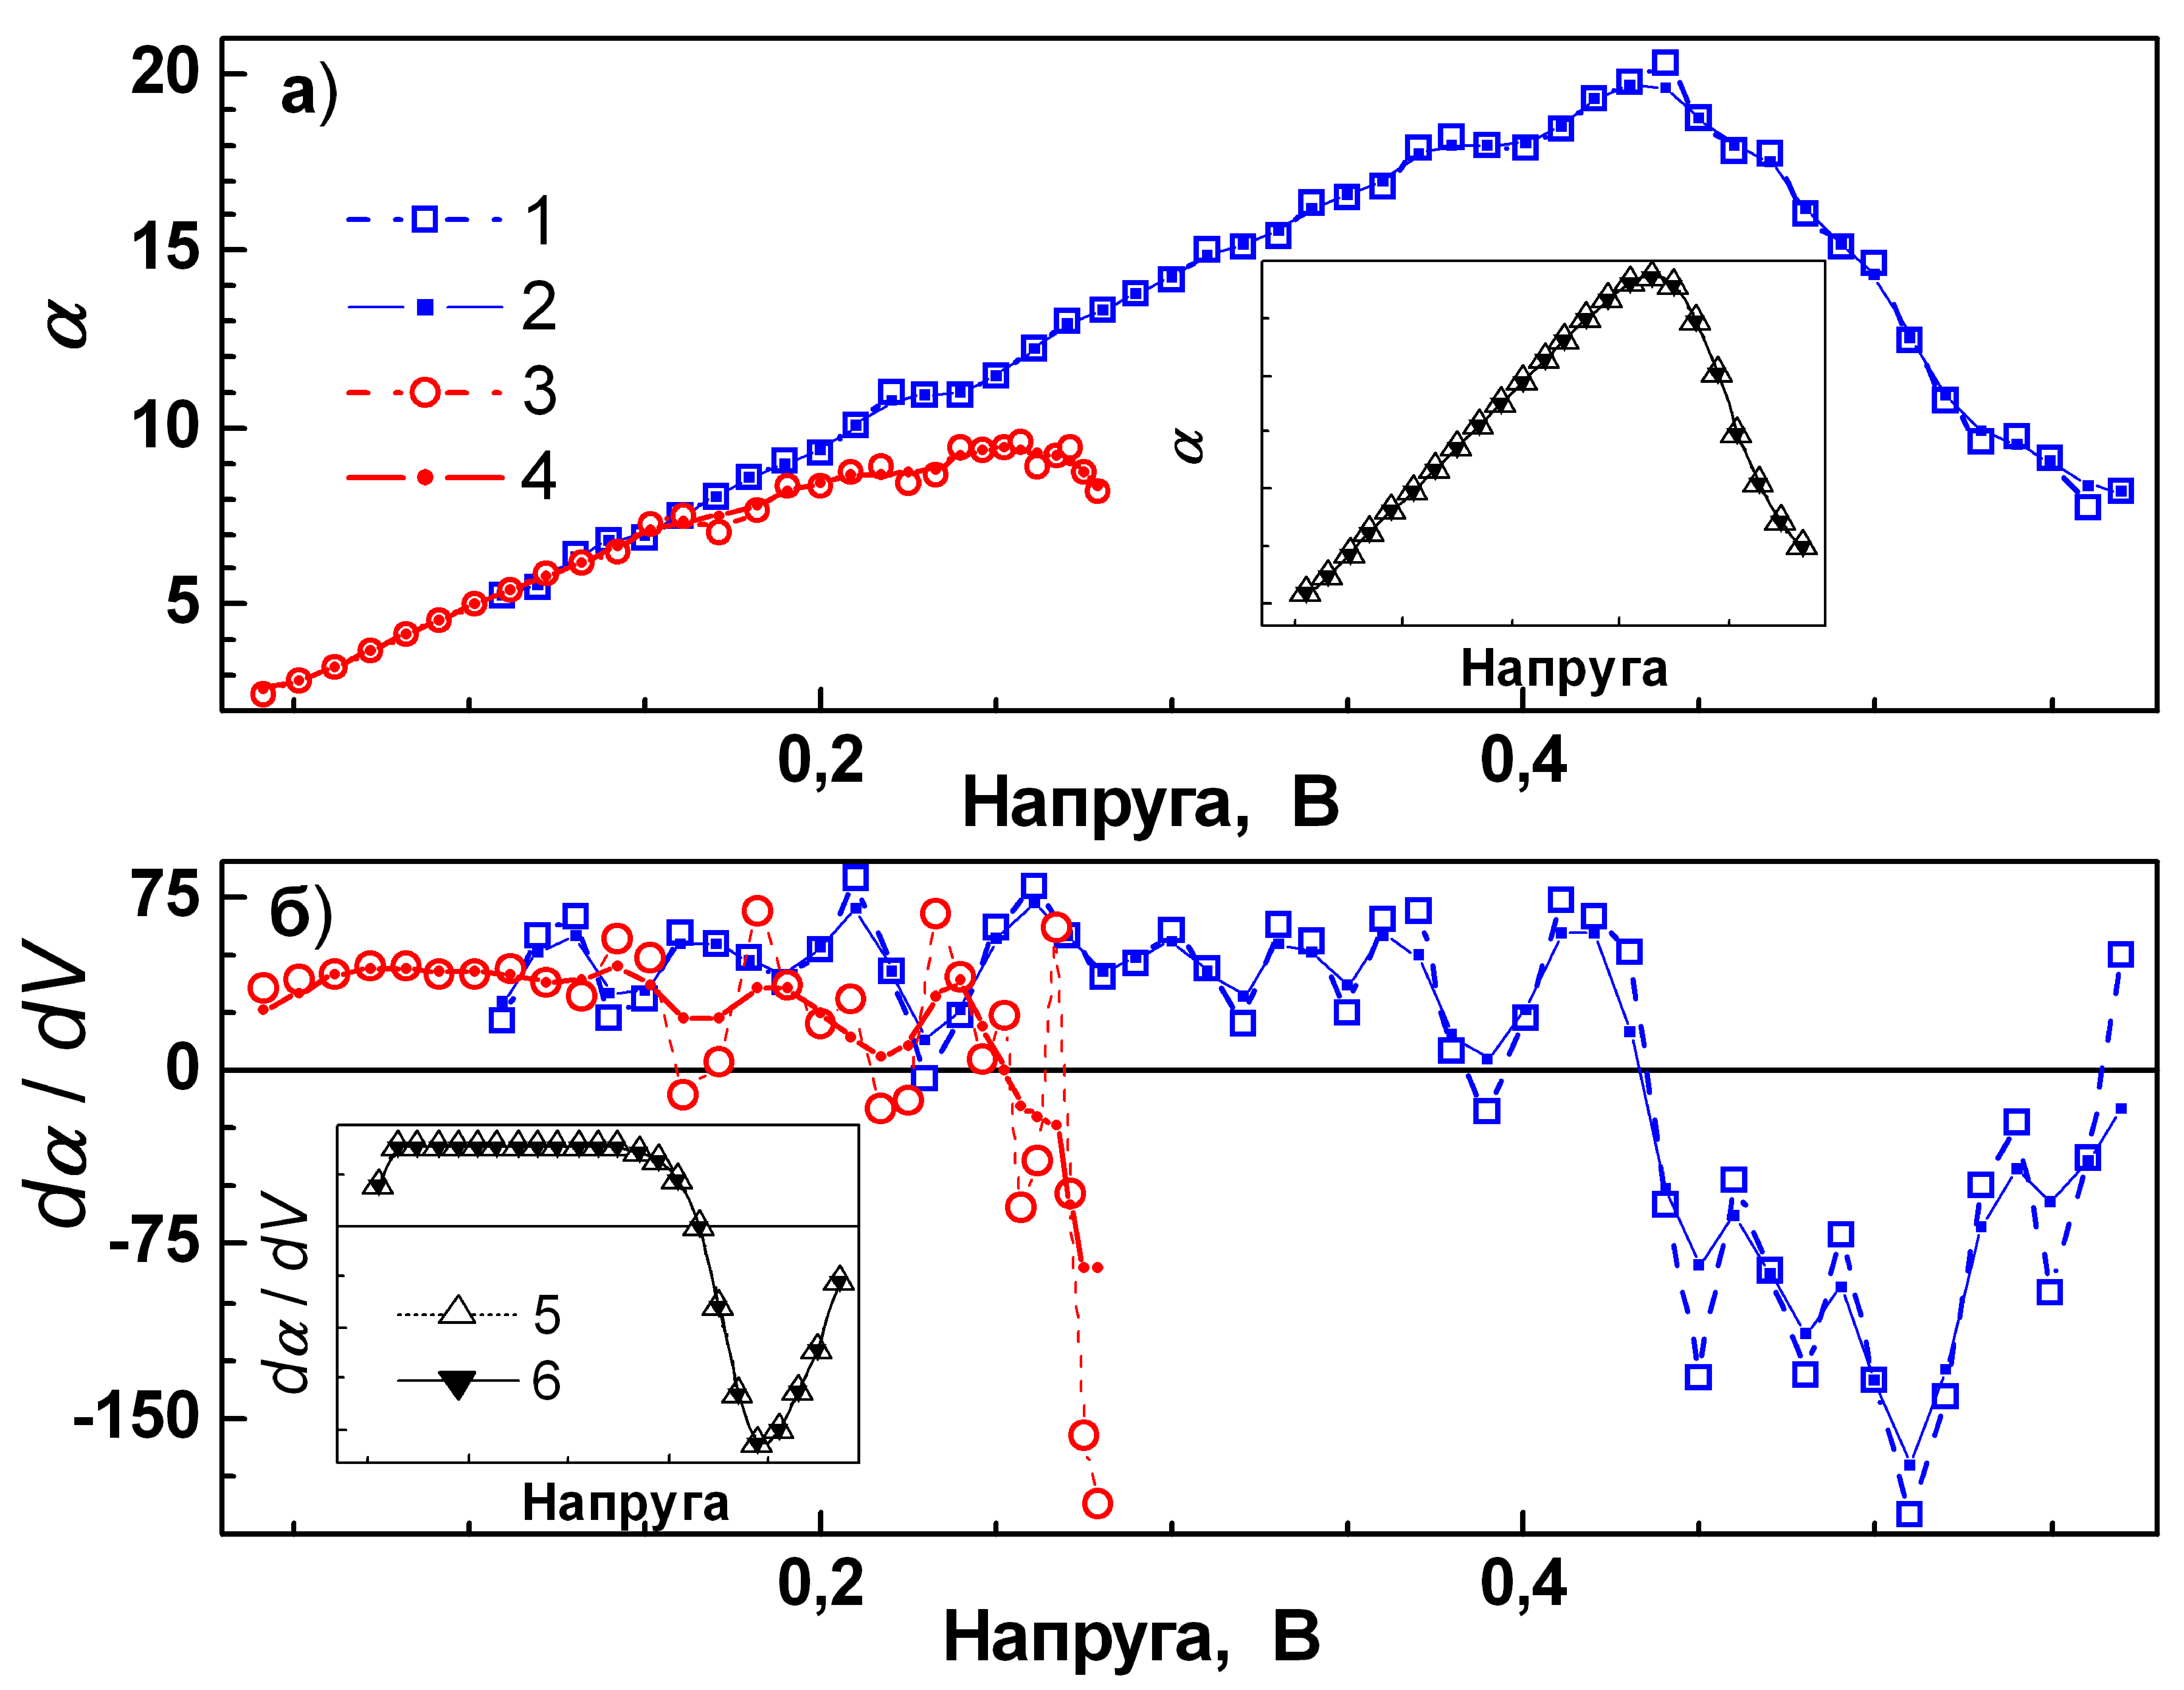
\includegraphics[width=1\textwidth]{figMikh}%
\caption{\label{figMikh}
Залежності функції~(\ref{eqMikh}) (а) та її похідної (б) від напруги.
Наведено графіки для зашумлених даних ($\sigma_V=0,3$~мВ, $\sigma_I^\varepsilon=1\%$, криві 1 та 2), для експериментально виміряних ВАХ (криві 3 та 4) та для ідеальних синтезованих ВАХ (вставка, криві 5 та 6) до (1, 3, 5) та після (2, 4, 6) запропонованої обробки.
}
\end{figure}

Зауважимо, що однією з необхідних властивостей методу, які використовуються для обчислення параметрів пристроїв з набору ВАХ, отриманих за різних умов, є можливість його застосування в автоматичному режимі.
В цьому випадку один з найпоширеніших варіантів пошуку екстремуму полягає у знаходженні нулів похідної.
Як видно з виразів (\ref{eqMikh})--(\ref{eqMikhDetFi}), для даного методу це означає необхідність проведення процедури чисельного знаходження другої похідної ВАХ.


Рис.~\ref{figMikh}(a) показує, що при використанні експериментальних ВАХ чи зашумлених даних чисельне диференціювання викликає появу багаточисленних локальних екстремумів на залежності функції $\alpha$ від $V$.
Ці екстремуми заважають автоматичному виявленню точки максимуму через наявність багатьох нульових точок на залежності $d\alpha/dV$ від $V$ --- див. Рис.~\ref{figMikh}(б).
З метою подолання цих труднощів, в роботі запропоновано проводити спеціальну 2-стадійну процедуру обробки даних.
А саме, на першій стадії обробки до отриманої з ВАХ залежності $\alpha$ від $V$ пропонується застосовувати 3--точковий медіанний фільтр, після чого, на другій стадії, проводити згладжування.
І лише після цього, проводити визначення положення максимуму, знаходження величин $\alpha_{max}$, $V_{max}$  та $I_{max}$ і розрахунок величин параметрів ДШ.
Дані на Рис.~\ref{figMikh} показують, що запропонована процедура обробки дійсно зменшує вплив побічних максимумів та дозволяє покращити точність методу.
Згладжування здійснюється завдяки усередненню по трьом сусіднім точкам з ваговими коефіцієнтами, які визначаються розподілом Гауса з дисперсією, рівною 0,6.

Надалі наведено результати, позначені міткою <<Mikhelashvili>> та отримані з використанням зазначеної процедури обробки.


\subsection{Чисельні методи}

The standard method of least squares with statistical weights is used.
Notably the parameters are determined by minimizing the sum of the vertical quadratic error:
\begin{equation}
\label{eqLS}
S(I_s,n,R_s)=\sum_{i=1}^{N_p}I_i^{-1}\left[I_i-I_{calc}(V_i,I_s,n,R_s)\right]^2,
\end{equation}
where $I_{calc}$ is the fitted values of the current.
The system of non-linear equations is solved by the coordinate-wise gradient descent method.
The criterion of the iterative procedure termination is $\mid(S_j-S_{j+1})/S_j\mid<10^{-12}$,
where $S_j$ is the error sum at $j-$th iteration.
The initial value of $R_s$ is derived by the intercept of the plot of $(dV/dI)/I$ vs $1/I$, which is constructed by using 5 last points of the $I$--$V$ data.
The initial values of $I_s$ and $n$ are evaluated from the plot of $\ln I$ vs $V$, which is corrected by initial $R_s$ value.

\subsection{Еволюційні алгоритми}


\section*{Висновки до розділу \ref{Ch_MSMethod}}
\addcontentsline{toc}{section}{Висновки до розділу \ref{Ch_MSMethod}}	
  \begin{enumerate}
     \item Проведено чисельний аналіз залежності величин похибок визначення ВБШ та послідовного опору в методі Норда від величини параметра $\gamma_N$ на масиві синтезованих ідеальних та зашумлених ВАХ.
     Виявлено, що похибка визначення висоти бар'ру зростає зі збільшенням параметру, тоді як залежність похибки оцінювання послідовного опору є немонотонною функцією $\gamma_N$.
     Показано, що найбільш оптимальним значенням є $\gamma_N=1,8$.
     \item Проведено чисельний аналіз залежності величин похибок визначення висоти бар'єру, фактору неідеальності та послідовного опору при використанні методу Бохліна від величин параметрів $\gamma_1$ та $\gamma_2$.
     Виявлено, що похибка екстрагування параметрів зростає при збільшенні величини $|\gamma_1-\gamma_2|$.
     Запропоновані оптимальні (для температурного діапазону $130\div330$~К) величини $\gamma_1=1,6$ та $\gamma_2=3,5$.
     \item Запропоновано адаптивну процедуру для вибору діапазону ВАХ, який використовується для побудови допоміжних функцій при застосуванні аналітичних методів визначення параметрів структур МН.
         Показано її ефективність на прикладі методу Громова.
     \item Запропоновано модифікацію методу Mikhelashvili, яка дозволяє застосовувати його в автоматичному режимі до набору ВАХ.
     Вона полягає у послідовному використанні медіанного фільтру та процедури згладжування функції $\alpha(V)=d(\ln I)/d(\ln V)$ перед знаходженням положення її максимуму.
     Показано доцільність застосування запропонованої процедури для підвищення точності методу.
  \end{enumerate}


\chapter{Оформление различных элементов} \label{chapt1}

\section{Форматирование текста} \label{sect1_1}

%\arabic{\curtextsize}

Мы можем сделать \textbf{жирный текст} и \textit{курсив}.

%\newpage
%============================================================================================================================

\section{Ссылки} \label{sect1_2}
Сошлёмся на библиографию.
\cite{Olikh:Visn2003,Olikh:SPQEO2003,Olikh:SEMT2004,Olikh:PJE2004,Olikh:PhChOM2005,
Olikh:PZTF2006,Olikh:MRS2007,Olikh:SEMT2007,Olikh:Visn2007,Olikh:FTP2009,Olikh:SPQEO2010,Gorb2010,
Olikh:UPJ2010,Olikh:SEMT2011,Olikh:FTP2011,Olikh:2013IEEE,Olikh:UPJ2013,Olikh:FTP2013,Olikh:SEMT2013,
Olikh:UPJ2014,Olikh:Ultras,OlikhJAP,Olikh:Rev,Olikh:Ultras2016,Olikh2016JSem,Olikh2018JAP,
1UNCPS,3Tomsk,1SEMST,50IUFFC,9APTTE,2005IUS,ICU2007SC,ICU2007GA,2007MRS,3UNCPS,6DrogGorb,6Drog,
12IvFr,4UNCPS,4Kremen,7Drog,5UNCPS,2012Ternop,14Plivk,8Drog,2013Buk,6UNCPS,2014IUSOl,2014IUS,6SEMST,
2015ICU,6CPFCS,7UNCPS,2017MEICS}
Одна ссылка: \cite[с.~54]{OlikhJAP}.
%\nocite{*}


%\include{Dissertation/part1}           % Глава 1
%\include{Dissertation/part2}           % Глава 2
%\include{Dissertation/part3}           % Глава 3
%\include{Dissertation/conclusion}      % Заключение
%\chapter*{Перелік умовних скорочень та позначень}             % Заголовок
\addcontentsline{toc}{chapter}{Перелік умовних скорочень та позначень}  % Добавляем его в оглавление
\noindent
%\begin{longtabu} to \dimexpr \textwidth-5\tabcolsep {r X}
\begin{longtabu} to \textwidth {r X}
  CDLR& coupled defect level recombination,  рекомбінація у системі спарених рівнів дефектів\\
  DE & differential evolution, метод диференційної еволюції \\
  FRC & fast--formed recombination center, швидко сформовані ВО дефекти \\
  NIEL & non--ionizing energy losses, втрати, не пов'язані з іонізацією \\
  MABC & modified artificial bee colony, метод  штучної бджолиної сім'ї\\
  OSFR & oxidization induced stacking--faults ring, кільцеві дефекти пакування, що виникли при окисненні \\
  PSO & particle swarm optimization, метод оптимізації зграї частинок\\
  RT & running time, час, необхідний для визначення параметрів\\
  SRC & slow--formed recombination center, повільно сформовані ВО дефекти\\
  TLBO & teaching learning based optimization, метод  оптимізованого викладання та навчання\\
  AAД & акусто--активний дефект\\
  АДВ & акусто--дефектна взаємодія \\
  АІ & акусто--індукований\\
  АХ & акустична хвиля\\
  АЧХ & амплітудно--частотна характеристика\\
  ВАХ & вольт--амперна характеристика\\
  ВБШ & висота бар'єру Шотки\\
  ВФХ & вольт--фарадна характеристика\\
  ГР &глибокий рівень \\
  ДШ & діод Шотки\\
  ЕА & еволюційний алгоритм\\
  КНО &  квазі--нейтральна область \\
  КП & кисневмісні преципітати\\
  КСЕ & кремнієвий сонячний елемент\\
  MH & метал--напівпровідник \\
  ОПЗ & область просторового заряду \\
  ППЗ & поперечний переріз захоплення \\
  РД & радіаційний дефект \\
  ТД &точковий дефект \\
  ТЕ & термоелектронна емісія \\
  ТПЕ & термопольова емісія \\
  УЗ & ультразвук \\
  УЗН & ультразвукове навантаження \\
  УЗО & ультразвукова обробка \\
  ШРХ & теорія Шоклі--Ріда--Хола  \\
$\alpha$ & коефіцієнт поглинання світла  \\
$\alpha_R$ & температурний коефіцієнт опору\\
$\beta$ & коефіцієнт квантового виходу  \\
$\beta_1$, $\beta_2$  & коефіцієнти Варшні  \\
$\Delta P$ & абсолютна АІ зміна параметра $P$\\
$\varepsilon$ & діелектрична проникність матеріалу  \\
$\varepsilon_0$ & діелектрична стала \\
$\varepsilon_P$ & відносна AI зміна параметра $P$\\
$\xi_\mathtt{US}$& амплітуда деформації ґратки при поширенні УЗ\\
$\vartheta$ & темп генерації РД\\
$\lambda$ &довжина хвилі падаючого світла\\
$\rho_\mathtt{LNO}$ & густина ніобату літію\\
$\rho_\mathtt{Si}$ & густина кремнію\\
$\sigma_\Phi0$ & стандартне відхилення висоти бар'єру при нульовому зміщенні\\
$\sigma_n$& поперечний переріз захоплення електронів дефектом\\
$\sigma_p$& поперечний переріз захоплення дірок дефектом\\
$\tau_{g}$ &ефективний час життя носіїв заряду в ОПЗ\\
$\tau_{n}$ &ефективний час життя електронів\\
$\tau_{n,\mathtt{RD}}$ & час життя електронів при рекомбінації на РД\\
$\upsilon_\mathtt{LNO}$ & швидкість звуку в ніобаті літію\\
$\upsilon_{\mathrm{th},n}$ & теплова швидкість електронів\\
$\upsilon_{\mathrm{th},p}$ & теплова швидкість дірок\\
$\upsilon_\mathtt{Si}$ & швидкість звуку в кремнії\\
$\Phi_b$ & ВБШ при нульовому зміщенні\\
$\Phi_{b}^0$ & середнє значення ВБШ при нульовому зміщенні (або ВБШ в однорідній області) \\
$\Psi$ & флюєнс опромінення\\
$\zeta$ & диференційний показник нахилу ВАХ \\
$A$ & площа зразка \\
$A_\mathtt{LNO}$ & площа п'єзоперетворювача\\
$A^*$ & ефективна стала Річардсона \\
$a_B$ & радіус Бора\\
$C$ & ємність діоду Шотки\\
$c$ & швидкість світла\\
$D$ & доза опромінення\\
$D_d$ & displacement damage dose, ефективна доза, пов'язана з дефектоутворенням\\
$E_g$ & ширина забороненої зони\\
$E_i$ & положення рівня Фермі у власному напівпровіднику\\
$E_t$ & положення енергетичного рівня, зв'язаного з дефектом\\
$F\!F$ & фактор форми освітленої ВАХ СЕ\\
$F_m$ & напруженість електричного поля на границі розділу метал-напівпровідник \\
$f_r$& резонансна частота п'єзоперетворювача\\
$f_\mathtt{US}$& частота УЗ\\
$h$, $\hbar$ & стала Планка\\
$I$ & струм\\
$I_s$ & струм насичення\\
$I_R$ & зворотний струм\\
$J$ & густина струму\\
$J_{ph}$ & густина фотогенерованого струму\\
$J_{sс}$ & густина струму короткого замикання\\
$k$ & стала Больцмана\\
$L_n$ & довжина дифузії електронів\\
$m*$ &  ефективна маса електрону \\
$N_c$ & ефективна густина станів біля дна зони провідності\\
$N_d$ & концентрація електронів поблизу контакту МН\\
$N_{t,\mathtt{RD}}$ & концентрація радіаційних дефектів\\
$N_v$ & ефективна густина станів біля вершини валентної зони\\
$n_i$ & концентрація власних носіїв заряду\\
$n$ & концентрація електронів\\
$n_\mathrm{id}$ & фактор неідеальності\\
$n_n$ & концентрація основних носіїв у електронному напівпровіднику \\
$n_p$ & концентрація неосновних носіїв у дірковому напівпровіднику \\
$q$ & елементарний заряд\\
$p$ & концентрація дірок \\
$p_n$ & концентрація неосновних носіїв у електронному напівпровіднику \\
$p_p$ & концентрація основних носіїв у дірковому напівпровіднику \\
$R$ & темп рекомбінації \\
$R_{\mathtt{DA}}$ & параметр зв'язку у моделі CDLR\\
$R_{ph}$ & коефіцієнт відбивання світла\\
$R_s$ & послідовний опір\\
$R_{sh}$ & шунтуючий опір\\
$T$ & абсолютна температура\\
$T_0$ & константа температурної залежності фактора неідеальності\\
$T_\mathtt{US}$ & період АХ\\
$t$ & час\\
$u_\mathtt{US}$&амплітуда зміщень атомів при поширенні УЗ\\
$V$ & напруга\\
$V_{bb}$ & вигин зон напівпровідника поблизу контакту\\
$V_d$ & падіння напруги в околі бар'ру\\
$V_n$ & різниця потенціалів між дном зони провідності та положенням рівня Фермі в об'ємі напівпровідника\\
$V_{oc}$ & напруга холостого ходу\\
$V_R$ & зворотна напруга\\
$V_\mathtt{RF}$ & амплітуда високочастотної напруги, прикладеної до п'єзоперетворювача\\
$W_{ph}$ & інтенсивність освітлення \\
$W_\mathtt{US}$ & інтенсивність акустичної хвилі\\

\end{longtabu}
\addtocounter{table}{-1}% Нужно откатить на единицу счетчик номеров таблиц, так как предыдующая таблица сделана для удобства представления информации по ГОСТ





        % Список сокращений и условных обозначений
%\include{Dissertation/dictionary}      % Словарь терминов
\begin{center}
%\section*{\MakeUppercase{ОСНОВНИЙ ЗМІСТ РОБОТИ}}
\textbf{\MakeUppercase{\fullbibtitle}}
\end{center}

\begin{enumerate}[label=\arabic*$^*$.,leftmargin=0em,itemindent=3em]
\item
Explanation of commonly observed shunt currents in c-Si solar cells by means of
  recombination statistics beyond the Shockley-Read-Hall approximation~/
  Silke~Steingrube, Otwin~Breitenstein, Klaus~Ramspeck et~al.~// \emph{J.
  Appl. Phys.} ---
  2011. --- July. ---
  Vol. 110, no.~1. ---
  P.~014515.



\item
\emph{Gopal,~Vishnu}. Contribution of Dislocations to the Zero-Bias
  Resistance-Area Product of {LWIR} {H}g{C}d{T}e Photodiodes at Low
  Temperatures~/ Vishnu~Gopal, Sudha~Gupta~// \emph{IEEE Trans. Electron
  Devices}. ---
  2004. --- Jul. ---
  Vol.~51, no.~7. ---
  P.~1078--1083.
  
\item
\emph{Mirzade,~Fikret}. Elastic wave propagation in a solid layer with
  laser-induced point defects~/ Fikret~Mirzade~// \emph{J. Appl. Phys.} ---
  2011. --- Sep. ---
  Vol. 110, no.~6. ---
  P.~064906.  

\item
Определение параметров глубоких уровней
  по дифференциальным коэффициентам
  вольт--амперных характеристик~/
  С.В.~Булярский, М.О.~Воробьев, Н.С.~Грушко,
  А.В.~Лакалин~// \emph{Письма в журнал
  технической физики}. ---
  1999. ---
  Т.~25, {№}~5. ---
  {С.}~22--27.

\item
\emph{Tung,~Raymond~T.} Recent advances in {S}chottky barrier concept~/
  Raymond~T.~Tung~// \emph{Materials Science and Engineering: R: Reports}.
  ---
  2001. --- Nov. ---
  Vol.~35, no. 1--3. ---
  P.~1--138.

\item
Distinction between the {P}oole-{F}renkel and tunneling models of
  electric-field-stimulated carrier emission from deep levels in
  semiconductors~/ S.~D.~Ganichev, E.~Ziemann, W.~Prettl et~al.~//
  \emph{Phys. Rev. B}. ---
  2000. --- Apr. ---
  Vol.~61, no.~15. ---
  P.~10361--10365.

\item
Schottky Barrier Height Inhomogeneity of Ti/n-GaAs Contact Studied by the I-V-T
  Technique~/ Yu-Long~Jiang, Guo-Ping~Ru, Fang~Lu et~al.~// \emph{Chin.
  Phys. Lett.} ---
  2002. --- Apr. ---
  Vol.~19, no.~4. ---
  P.~553--556.

\item
\emph{Brailsford,~A.~D.} Abrupt--Kink Model of Dislocation Motion~/
  A.~D.~Brailsford~// \emph{Phys. Rev.} ---
  1961. --- May. ---
  Vol. 122, no.~3. ---
  P.~778--786.

\item
\emph{Pipinys,~P.} Temperature dependence of reverse--bias leakage current
  in {G}a{N} {S}chottky diodes as a consequence of phonon--assisted tunneling~/
  P.~Pipinys, V.~Lapeika~// \emph{J. Appl. Phys.} ---
  2006. --- May. ---
  Vol.~99, no.~9. ---
  P.~093709.

\item
\emph{Jafar,~M M Abdul-Gader}. High-bias current--voltage--temperature
  characteristics of undoped rf magnetron sputter deposited boron carbide
  ({B}$_5${C})/p--type crystalline silicon heterojunctions~/ M~M
  Abdul-Gader~Jafar~// \emph{Semicond. Sci. Technol.} ---
  2003. --- Jan. ---
  Vol.~18, no.~1. ---
  P.~7--22.
\end{enumerate}
      % Список литературы
%\include{Dissertation/lists}           % Списки таблиц и изображений (иллюстративный материал)
%%\input{Dissertation/appendixsetup}   % Предварительные настройки для правильного подключения Приложений
%\chapter{\MakeUppercase{список публікацій за темою дисертації}} \label{AppendixA}
\chapter*{\MakeUppercase{Додатки}}						% Заголовок
\addcontentsline{toc}{chapter}{\MakeUppercase{Додатки}}
\section*{Додаток А. Список публікацій за темою дисертації та відомості про апробацію результатів}


\begin{center}%
\emph{Наукові праці, в яких опубліковано основні наукові результати дисертації}
\end{center}%
%\subsection*{Наукові праці, в яких опубліковано основні наукові результати дисертації}
\begin{enumerate}[label=\arabic*.,leftmargin=1em,itemindent=1em]
%\begin{enumerate}[label=\arabic*.,leftmargin=0em,itemindent=2em]
%\setcounter{enumi}{25}
\item
Acousto--defect interaction in irradiated and non--irradiated silicon
  $n^+$--$p$ structure~/ O.~Ya.~Olikh, A.~M.~Gorb, R.~G.~Chupryna,
  O.~V.~Pristay-Fenenkov~// \emph{J. Appl. Phys.} --- 2018. --- Apr. ---
 Vol. 123, no.~16. --- P.~161573--1--161573--12.

\item
\emph{Olikh,~O.Ya.} Acoustically driven degradation in single crystalline
  silicon solar cell~/ O.Ya.~Olikh~// \emph{Superlattices Microstruct.} ---
  2018. --- May. ---
  Vol. 117. ---
  P.~173--188.

\item
\emph{Olikh,~Oleg}. On the mechanism of ultrasonic loading effect in
  silicon--based {S}chottky diodes~/ Oleg~Olikh, Katerina~Voytenko~//
  \emph{Ultrasonics}. ---
  2016. --- Mar. ---
  Vol.~66, no.~1. ---
  P.~1--3.

\item
Effect of ultrasound on reverse leakage current of silicon {S}chottky barrier
  structure~/ O.~Ya.~Olikh, K.~V.~Voytenko, R.~M.~Burbelo, Ja.~M.~Olikh~//
  \emph{Journal of Semiconductors}. ---
  2016. --- Dec. ---
  Vol.~37, no.~12. ---
  P.~122002--1--122002--7.

\item
\emph{Olikh,~O.~Ya.} Review and test of methods for determination of the
  {S}chottky diode parameters~/ O.~Ya.~Olikh~// \emph{J. Appl. Phys.} ---
  2015. --- Jul. ---
  Vol. 118, no.~2. ---
  P.~024502--1--024502--14.

\item
\emph{Olikh,~O.~Ya.} Ultrasound influence on {I}--{V}--{T} characteristics
  of silicon {S}chottky barrier structure~/ O.~Ya.~Olikh, K.~V.~Voytenko,
  R.~M.~Burbelo~// \emph{J. Appl. Phys.} ---
  2015. --- Jan. ---
  Vol. 117, no.~4. ---
  P.~044505--1--044505--7.

\item
\emph{Olikh,~Oleg}. Reversible influence of ultrasound on
  $\gamma-$irradiated {M}o/n-{S}i {S}chottky barrier structure~/ Oleg~Olikh~//
  \emph{Ultrasonics}. ---
  2015. --- Feb. ---
  Vol.~56. ---
  P.~545--550.

\item
Особливості дислокаційного поглинання
  ультразвуку в безсубблочних кристалах
  {C}d$_{0,2}${H}g$_{0,8}${T}e~/ І.~О.~Лисюк, Я.~М.~Оліх,
  О.~Я.~Оліх, Г.~В.~Бекетов~// \emph{УФЖ}. ---
  2014. ---
  Т.~59, {№}~1. ---
  {С.}~50--57.

\item
\emph{Olikh,~O.~Ya.} Non-Monotonic $\gamma-$Ray Influence on {M}o/n-{S}i
  {S}chottky Barrier Structure Properties~/ O.~Ya.~Olikh~// \emph{IEEE
  Trans. Nucl. Sci.} ---
  2013. --- Feb. ---
  Vol.~60, no.~1. ---
  P.~394--401.

\item
\emph{Оліх,~О.~Я.} Особливості впливу
  ультразвуку на перенесення заряду в
  кремнієвих структурах з бар’єром {Ш}отки
  залежно від дози $\gamma$--опромінення~/
  О.~Я.~Оліх~// \emph{Сенсорна електроніка і
  мікросистемні технології}. ---
  2013. ---
  Т.~10, {№}~1. ---
  {С.}~47--55.

\item
\emph{Олих,~О.~Я.} Влияние ультразвукового
  нагружения на протекание тока в
  структурах {M}o/n--n$^+$--{S}i c барьером {Ш}оттки~/
  О.~Я.~Олих~// \emph{Физика и техника
  полупроводников}. ---
  2013. ---
  Т.~47, {№}~7. ---
  {С.}~979--984.

\item
\emph{Оліх,~О.~Я.} Особливості перенесення
  заряду в структурах {M}o/n--{S}i з бар’єром
  {Ш}отки~/ О.~Я.~Оліх~// \emph{УФЖ}. ---
  2013. ---
  Т.~58, {№}~2. ---
  {С.}~126--134.

\item
\emph{Олих,~О.~Я.} Особенности динамических
  акустоиндуцированных изменений
  фотоэлектрических параметров кремниевых
  солнечных элементов~/ О.~Я.~Олих~//
  \emph{Физика и техника полупроводников}. ---
  2011. ---
  Т.~45, {№}~6. ---
  {С.}~816--822.

\item
\emph{Оліх,~Я.~М.} Інформаційний чинник
  акустичної дії на структуру дефектних
  комплексів у напівпровідниках~/ Я.~М.~Оліх,
  О.~Я.~Оліх~// \emph{Сенсорна електроніка і
  мікросистемні технології}. ---
  2011. ---
  Т. 2(8), {№}~2. ---
  {С.}~5--12.

\item
\emph{Оліх,~О.~Я.} Особливості впливу
  нейтронного опромінення на динамічну
  акустодефектну взаємодію у кремнієвих
  сонячних елементах~/ О.~Я.~Оліх~// \emph{УФЖ}.
  ---
  2010. ---
  Т.~55, {№}~7. ---
  {С.}~770--776.


\item
Ultrasonically Recovered Performance of $\gamma-$Irradiated Metal-Silicon
  Structures~/ A.M.~Gorb, O.A.~Korotchenkov, O.Ya~Olikh, A.O.~Podolian~//
  \emph{IEEE Trans. Nucl. Sci.} ---
  2010. --- June. ---
  Vol.~57, no.~3. ---
  P.~1632--1639.

\item
\emph{Олих,~О.~Я.} Изменение активности
  рекомбинационных центров в кремниевых
  p--n--структурах в условиях акустического
  нагружения~/ О.~Я.~Олих~// \emph{Физика и
  техника полупроводников}. ---
  2009. ---
  Т.~43, {№}~6. ---
  {С.}~774--779.

\item
\emph{Оліх,~О.~Я.} Робота кремнієвих сонячних
  елементів в умовах акустичного
  навантаження мегагерцового діапазону~/
  О.~Я.~Оліх, Р.~М.~Бурбело, М.~К.~Хіндерс~//
  \emph{Сенсорна електроніка і
  мікросистемні технології}. ---
  2007. ---
  Т.~4, {№}~3. ---
  {С.}~40--45.

\item
\emph{Olikh,~O.Ya.} The Dynamic Ultrasound Influence on Diffusion and Drift
  of the Charge Carriers in Silicon p--n Structures~/ O.Ya.~Olikh, R.~Burbelo,
  M.~Hinders~// Semiconductor Defect Engineering --- Materials, Synthetic,
  Structures and Devices II~/ Ed. by S.~Ashok, P.~Kiesel, J.~Chevallier,
  T.~Ogino. ---
  Vol.~994 of \emph{Materials Research Society Symposium
  Proceedings}. ---
  Warrendale, PA: 2007. ---
  P.~269--274.

\item
\emph{Олих,~О.~Я.} Акустостимулированные
  коррекции вольт--амперных характеристик
  арсенид--галлиевых структур с контактом
  {Ш}оттки~/ О.~Я.~Олих, Т.~Н.~Пинчук~//
  \emph{Письма в Журнал Технической Физики}.
  ---
  2006. ---
  Т.~32, {№}~12. ---
  {С.}~22--27.

\item
\emph{Конакова,~Р.В.} Влияние микроволновой
  обработки на уровень остаточной
  деформации и параметры глубоких уровней
  монокристаллах карбида кремния~/
  Р.В.~Конакова, П.М.~Литвин, О.Я.~Олих~//
  \emph{Физика и химия обработки материалов}.
  ---
  2005. ---
  {№}~2. ---
  {С.}~19--22.


\item
\emph{Конакова,~Р.В.} Влияние микроволновой
  обработки на глубокие уровни
  монокристаллов {G}a{A}s и {S}i{C}~/ Р.В.~Конакова,
  П.М.~Литвин, О.Я.~Олих~// \emph{Петербургский
  журнал электроники}. ---
  2004. ---
  {№}~1. ---
  {С.}~20--24.

\item
\emph{Olikh,~Ja.~М.} Active ultrasound effects in the future usage in
  sensor electronics~/ Ja.~М.~Olikh, O.Ya.~Olikh~// \emph{Сенсорна
  електроніка і мікросистемні технології}.
  ---
  2004. ---
  Т.~1, {№}~1. ---
  {С.}~19--29.

\item
\emph{Olikh,~O.Ya.} Acoustoelectric transient spectroscopy of microwave
  treated {G}a{A}s--based structures~/ O.Ya.~Olikh~// \emph{Semiconductor
  Physics, Quantum Electronics \& Optoelectronics}. ---
  2003. ---
  Vol.~6, no.~4. ---
  P.~450--453.

\item
\emph{Оліх,~О.Я.} Акустостимульовані
  динамічні ефекти в сонячних елементах на
  основі кремнію~/ О.Я.~Оліх~// \emph{Вісник
  Київського ун-ту, Сер.: Фізико-математичні
  науки}. ---
  2003. ---
  {№}~4. ---
  {С.}~408--414.
\end{enumerate}

\begin{center}%
\emph{Наукові праці, які засвідчують апробацію матеріалів дисертації}
\end{center}%
\begin{enumerate}[label=\arabic*.,leftmargin=1em,itemindent=1em]
\setcounter{enumi}{25}
\item
\emph{Оліх,~О.~Я.} Ефекти активного
  ультразвуку в напівпровідникових
  кристалах~/ О.~Я.~Оліх~// 1--а {У}країнська
  наукова конференція з фізики
  напівпровідників, {О}деса, {У}країна. ---
  Т.~1. ---
  Одеса: 2002. ---
  {С.}~80.

\item
Влияние {СВЧ} облучения на остаточный
  уровень внутренних механических
  напряжений и параметры глубоких уровней в
  эпитак-сиальных структурах {G}a{A}s~/
  Р.~В.~Конакова, А.~Б.~Камалов, О.~Я.~Олих
  {и~др.}~// Труды {III} международной
  конференции <<{Р}адиационно--термические
  эффекты и процессы в неорганических
  материалах>>, {Т}омск, {Р}оссия. ---
  Томск: 2002. ---
  {С.}~338--339.

\item
\emph{Оліх,~О.~Я.} Про роль теплових і
  деформаційних механізмів дії ультразвуку
  на роботу кремнієвих сонячних елементів~/
  О.~Я.~Оліх~// Міжнародна науково--технічна
  конференція <<{С}енсорна електроніка і
  мікросистемні технології {СЕМСТ}--1>>,
  {О}деса, {У}країна. Тези доповідей. ---
  Одеса: 2004. ---
  {С.}~163.

\item
\emph{Olikh,~O.} Investigation of microwave treated epitaxial {G}a{A}s
  structures by acoustoelectric method~/ O.~Olikh~// 2004 {IEEE}
  {I}nternational {U}ltrasonics, {F}erroelectrics and {F}requency {C}ontrol
  {J}oint 50$^{th}$ {A}nniversary {C}onference. Montreal, {C}anada. Abstracts.
  ---
  Montreal: 2004. ---
  Pp.~230--231.

\item
\emph{Олих,~О.~Я.} Влияние {СВЧ} облучения на
  остаточный уровень внутренних
  механических напряжений и параметры
  глубоких уровней в эпитак-сиальных
  структурах {G}a{A}s~/ О.~Я.~Олих~// Труды девятой
  международной научно--технической
  конференции <<{А}ктуальные проблемы
  твердотельной электроники и
  микроэлектроники>>, {Д}ивноморское,
  {Р}оссия. ---
  Дивноморское: 2004. ---
  {С.}~278--279.

\item
Influence of acoustic wave on forming and characteristics of silicon p--n
  junction~/ J.~Olikh, A.~Evtukh, B.~Romanyuk, O.~Olikh~// 2005 {IEEE}
  {I}nternational {U}ltrasonics {S}ymposium and {S}hort {C}ourses. Rotterdam,
  {N}etherlands. Abstracts. ---
  Rotterdam: 2005. ---
  P.~542.

\item
\emph{Olikh,~O.} Dynamic ultrasound effects in silicon solar sell~/
  O.~Olikh, R.~Burbelo, Hinders~M.~// 2007 {I}nternational {C}ongress on
  {U}ltrasonics. {P}rogram and {B}ook of {A}bstracts. {V}ienna, {A}ustria. ---
  Vienna: 2007. ---
  P.~94.

\item
\emph{Olikh,~O.} Influence of the ultrasound treatment on
  {A}u-{T}i{B}--n--n$^+$--{G}a{A}s structure electrical properties~/
  O.~Olikh~// 2007 {I}nternational {C}ongress on {U}ltrasonics. {P}rogram and
  {B}ook of {A}bstracts. {V}ienna, {A}ustria. ---
  Vienna: 2007. ---
  P.~94.

\item
\emph{Olikh,~O.} The Dynamic Ultrasound In-fluence on Diffusion and Drift of
  the Charge Carriers in Silicon p--n Structures~/ O.~Olikh, R.~Burbelo,
  M.~Hinders~// {MRS} 2007 {S}pring {M}eeting, {S}ymposium {F}: {S}emiconductor
  {D}efect {E}ngineering --- {M}aterials, {S}ynthetic {S}tructures, and
  {D}evices {II}. San {F}rancisco, {USA}. ---
  San {F}rancisco: 2007. ---
  P.~3.11.

\item
\emph{Оліх,~О.~Я.} Робота кремнієвих сонячних
  елементів в умовах акустичного
  навантаження мегагерцового діапазону~/
  О.~Я.~Оліх~// {ІІІ} {У}країнська наукова
  конференція з фізики напівпровідників
  {УНКФН}--3, {О}деса, {У}країна. Тези доповідей.
  ---
  Одеса: 2007. ---
  {С.}~322.

\item
\emph{Оліх,~О.~Я.} Вплив ультразвукової
  обробки на вольт--амперні характеристики
  опромінених кремнієвих структур~/
  О.~Я.~Оліх, А.~М.~Горб~// {VІ} {М}іжнародна
  школа--конференція <<Актуальні проблеми
  фізики напівпровідників>>, {Д}рогобич,
  {У}країна. Тези доповідей. ---
  Дрогобич: 2008. ---
  {С.}~114.

\item
\emph{Оліх,~О.~Я.} Акустичні збурення
  дефектної підсистеми кремнієвих
  p--n--структур~/ О.~Я.~Оліх~// {VІ} {М}іжнародна
  школа--конференція <<Актуальні проблеми
  фізики напівпровідників>>, {Д}рогобич,
  {У}країна. Тези доповідей. ---
  Дрогобич: 2008. ---
  {С.}~174.


\item
\emph{Оліх,~О.~Я.} Особливості механізму
  ультразвукового впливу на
  фото--електричний струм у
  нейтронно--опромінених {S}i--p--n--структурах~/
  О.~Я.~Оліх~// {IV} {У}країнська наукова
  конференція з фізики напівпровідників,
  {З}апоріжжя, {У}країна. Тези доповідей. ---
  Т.~2. ---
  {З}апоріжжя: 2009. ---
  {С.}~59.

  \item
\emph{Olikh,~O.} Ultrasound influence on the recombination centers in
  silicon p-n--structures~/ O.~Olikh~// 13th International Conference on
  Defects --- Recognition, Imaging and Physics in Semiconductors. Wheeling,
  {USA}. Final program. ---
Wheeling: 2009. ---
Pp.~9--10.


\item
\emph{Оліх,~Я.~М.} Про можливості практично-го
  застосування ультразвуку для керування
  характеристиками перетворювачів
  сонячної енергії~/ Я.~М.~Оліх, О.~Я.~Оліх~//
  Четверта міжнародна науково--практична
  конференція <<Матеріали електронної
  техніки та сучасні інформаційні
  технології>>, {К}ременчук, {У}країна. Тези
  доповідей. ---
  {К}ременчук: 2010. ---
  {С.}~147--148.

\item
\emph{Оліх,~О.~Я.} Немонотонний вплив
  $\gamma$--опромінення на електричні
  властивості кремнієвих структур з
  бар’єром {Ш}отки~/ О.~Я.~Оліх, С.~В.~Онисюк~//
  {VІI} {М}іжнародна школа--конференція
  <<Актуальні проблеми фізики
  напівпровідників>>, {Д}рогобич, {У}країна.
  Тези доповідей. ---
  Дрогобич: 2010. ---
  {С.}~171--172.

\item
\emph{Оліх,~О.~Я.} Особливості динамічного
  ультразвукового впливу на
  $\gamma$--опромінені кремнієві $m-s-$структури~/
  О.~Я.~Оліх, С.~В.~Онисюк~// Збірник тез {V}
  {У}країнської наукової конференції з
  фізики напівпровідників {УНКФН}--5,
  Ужгород, {У}країна. ---
  Ужгород: 2011. ---
  {С.}~339--340.

\item
\emph{Оліх,~О.~Я.} Вплив ультразвуку на
  термоемісійні процеси в Mo/n--n$^+$--Si
  структурах~/ О.~Я.~Оліх~// Матеріали
  {В}сеукраїнської наукової конференції
  <<Актуальні проблеми теоретичної,
  експериментальної та прикладної фізики>>,
  {Т}ернопіль, {У}країна. ---
  Тернопіль: 2012. ---
  {С.}~101--103.

\item
\emph{Olikh,~O.~Ya.} Reversible Alteration of Reverse Current in Mo/n--Si
  Structures Under Ultrasound Loading~/ O.~Ya.~Olikh, Ya.~M.~Olikh~//
  Фізика і технологія тонких плівок та
  наносистем. {М}атеріали {ХІV} Міжнародної
  конференції~/ {Під ред. }Д.М.~Фреїкa. ---
  Івано--Франківськ: Видавництво
  {П}рикарпатського національного
  університету імені {В}асиля {С}тефаника,
  2013. ---
  {С.}~322.

\item
\emph{Olikh,~O.~Ya.} Modification of reverse current in the Mo/n--Si
  structures under conditions of ultrasonic loading~/ O.~Ya.~Olikh,
  K.~V.~Voytenko~// {VІІI} {I}nternational school--conference <<Actual
  problems of semiconductor physics>>, {D}rohobych, {U}kraine. Abstract book.
  ---
  Drohobych: 2013. ---
  Pp.~101--102.

\item
\emph{Olikh,~Ya.~M.} About acoustical--stimulated a self--organization
  defect structures in semiconductor during ion implantation~/ Ya.~M.~Olikh,
  O.~Ya.~Olikh~// International research and practice conference
  <<Nanotechnology and nanomaterials>>, {B}ukovel, {U}kraine. Abstract book.
  ---
  Bukovel: 2013. ---
  P.~240.

\item
\emph{Оліх,~О.~Я.} Вплив $\gamma$--опромінення на
  механізм перенесення заряду в структурах
  Mo/n--Si~/ О.~Я.~Оліх~// {VІ} {У}країнська наукова
  конференція з фізики напівпровідників
  {УНКФН}--6. Чернівці, {У}країна. Тези
  доповідей. ---
  Чернівці: 2013. ---
  {С.}~121--122.

\item
\emph{Olikh,~Ya.} New approach to ultrasonic absorption in subgrain--free
  {C}d$_{0,2}${H}g$_{0,8}${T}e crystals~/ Ya.~Olikh, I.~Lysyuk, O.~Olikh~//
  2014 {IEEE} {I}nternational {U}ltrasonics {S}ymposium. Chicago, {I}llinois,
  {USA}. Abstract book. ---
  Chicago: 2014. ---
  Pp.~439--440.

\item
\emph{Olikh,~O.} Ultrasonically induced effects in {S}chottky barrier
  structure depending on a $\gamma$--irradiation~/ O.~Olikh~// 2014 {IEEE}
  {I}nternational {U}ltrasonics {S}ymposium. Chicago, {I}llinois, {USA}.
  Abstract book. ---
  Chicago: 2014. ---
  Pp.~645--646.

\item
\emph{Оліх,~О.~Я.} Характеризація
  $\gamma$--опромінених кремнієвих p--n--структур
  методом диференційних коефіцієнтів~/
  О.~Я.~Оліх, О.~В.~Пристай~// 6--та Міжнародна
  науково--технічна конференція <<{С}енсорна
  електроніка і мікросистемні технології>>,
  {О}деса, {У}країна. Тези доповідей. ---
  Одеса: 2014. ---
  {С.}~193.

\item
\emph{Olikh,~O.Ya}. Ultrasonic Loading Effects on Silicon--based Schottky
  Diodes~/ O.Ya~Olikh, K.~V.~Voytenko~// 2015 {I}nternational {C}ongress on
  {U}ltrasonics. Metz, {F}rance. Abstract book. ---
  Metz: 2015. ---
  P.~225.

\item
\emph{Оліх,~О.~Я.} Порівняння ефективності
  методів визначення параметрів діодів
  {Ш}отки~/ О.~Я.~Оліх~// Сучасні проблеми
  фізики конденсованого стану: {П}раці {IV}--ї
  міжнародної конференції. {К}иїв, {У}країна.
  ---
  Київ: 2015. ---
  {С.}~32--34.

\item
Ультразвукова модифікація стимульованого
  фононами тунелювання у кремнієвих діодах
  Шотки~/ О.~Я.~Оліх, К.~В.~Войтенко,
  Р.~М.~Бурбело, Я.~М.~Оліх~// {VІI} {У}країнська
  наукова конференція з фізики
  напівпровідників {УНКФН}--7. Дніпро,
  {У}країна. Тези доповідей. ---
  Дніпро: 2016. ---
  {С.}~190--191.

\item
\emph{Оліх,~О.~Я.} Акусто--керована
  модифікація властивостей кремнієвих
  фотоелектроперетворювачів~/ О.~Я.~Оліх~//
  Перспективні напрямки сучасної
  електроніки, інформаційних і
  комп’ютерних систем. Тези доповідей на
  {ІІ} Всеукраїнській науково--практичній
  конференції {МЕІСS}--2017. Дніпро, {У}країна. ---
  Дніпро: 2017. ---
  {С.}~302--303.
\end{enumerate}


\begin{center}%
\emph{Апробація результатів дисертації}
\end{center}%
\begin{enumerate}[label=\arabic*.,leftmargin=1em,itemindent=1em]

\item
1--а Українська наукова конференція з фізики напівпровідників, Одеса, Україна, 2002~р., очна форма участі.

\item
III международная конференция <<Радиационно--термические эффекты и процессы в неорганических материалах>>, Томск, Россия, 2002~р., заочна форма участі.

\item
Міжнародна науково-технічна конференція <<Сенсорна електроніка і мікросистемні технології СЕМСТ--1>>, Одеса, Україна, 2004~р., очна форма участі.

\item
2004 IEEE International Ultrasonics, Ferroelectrics and Frequency Control Joint 50th Anniversary Conference, Montreal, Canada, 2004~р., очна форма участі.

\item
Девятая международная научно-техническая конференция <<Актуальные проблемы твердотельной электроники и микроэлектроники>>, Дивноморское, Россия, 2004~р., заочна форма участі.

\item
2005 IEEE International Ultrasonics Symposium and Short Courses, Rotterdam, Netherlands, 2005~р., заочна форма участі.

\item
2007 International Congress on Ultrasonics, Vienna, Austria, 2007~р., очна форма участі.

\item
MRS 2007 Spring Meeting, Symposium F: Semiconductor Defect Engineering --- Materials, Synthetic Structures, and Devices II. San Francisco, USA, 2007~р., очна форма участі.

\item
ІІІ Українська наукова конференція з фізики напівпровідників УНКФН--3, Одеса, Україна, 2007~р., заочна форма участі.

\item
VІ Міжнародна школа--конференція <<Актуальні проблеми фізики напівпровідників>>, Дрогобич, Україна, 2008~р., очна форма участі.

\item
ХІІ Міжнародна конференція <<Фізика і технологія тонких плівок та наносистем>>, Івано--Франківськ, Україна, 2009~р., заочна форма участі.

\item
IV Українська наукова конференція з фізики напівпровідників, Запоріжжя, Україна, 2009~р., очна форма участі.

\item
13th International Conference on Defects --- Recognition, Imaging and Physics in Semiconductors, Wheeling, USA, 13--17 вересня, 2009~р., заочна форма участі.

\item
Четверта міжнародна науково--практична конференція <<Матеріали електронної техніки та сучасні інформаційні технології>>, Кременчук, Україна, 2010~р., заочна форма участі.

\item
VІІ Міжнародна школа-конференція <<Актуальні проблеми фізики напівпровідників>>, Дрогобич, Україна, 2010~р., заочна форма участі.

\item
V Українська наукова конференція з фізики напівпровідників УНКФН--6, Ужгород, Україна, 9--15 жовтня, 2011~р., заочна форма участі.

\item
Всеукраїнська наукова конференція <<Актуальні проблеми теоретичної, експериментальної та прикладної фізики>>, Тернопіль, Україна, 2012~р., заочна форма участі.

\item
ХІV Міжнародна конференція <<Фізика і технологія тонких плівок та наносистем>>, Буковель, Україна, 20--25 травня, 2013~р., заочна форма участі.

\item
VІІI Міжнародна школа--конференція <<Актуальні проблеми фізики напівпровідників>>, Дрогобич, Україна, 2013~р., заочна форма участі.

\item
International research and practice conference <<Nanotechnology and nanomaterials>>, Bukovel, Ukraine, 2013~р., заочна форма участі.

\item
VІ Українська наукова конференція з фізики напівпровідників УНКФН--6, Чернівці, Україна, 30 вересня -- 4 жовтня, 2013~р., очна форма участі.

\item
2014 IEEE International Ultrasonics Symposium, Chicago, USA, 2014~р., заочна форма участі.

\item
6--та Міжнародна науково--технічна конференція <<Сенсорна електроніка і мікросистемні технології>>, Одеса, Україна, 2014~р., заочна форма участі.

\item
2015 International Congress on Ultrasonics. Metz, France, 2015~р., очна форма участі.

\item
IV міжнародна конференція <<Сучасні проблеми фізики конденсованого стану>>, Київ, Україна, 2015~р., очна форма участі.

\item
VІІ Українська наукова конференція з фізики напівпровідників УНКФН--7, Дніпро, Україна, 26--30 вересня 2016~р., заочна форма участі.


\item
ІІ Всеукраїнська науково-практична конференція <<Перспективні напрямки 
сучасної електроніки, 
інформаційних і комп'ютерних 
систем>> МЕІСS-2017, Дніпро, Україна, 22--24 листопада 2017~р., заочна форма участі.

\end{enumerate}
%печатаемых сообщениях), он представлен на листинге~\ref{list:hwbeauty}.
%\begin{ListingEnv}[!h]% настройки floating аналогичны окружению figure
%    \captiondelim{ } % разделитель идентификатора с номером от наименования
%    \caption{Программа ,,Hello, world`` на \protect\cpp}
%    % далее метка для ссылки:
%    \label{list:hwbeauty}
%    % окружение учитывает пробелы и табуляции и применяет их в сответсвии с настройками
%    \begin{lstlisting}[language={[ISO]C++}]
%	#include <iostream>
%	using namespace std;
%
%	int main() //кириллица в комментариях при xelatex и lualatex имеет проблемы с пробелами
%	{
%		cout << "Hello, world" << endl; //latin letters in commentaries
%		system("pause");
%		return 0;
%	}
%    \end{lstlisting}
%\end{ListingEnv}%
%Второй не~такой красивый, но без ограничений (см.~листинг~\ref{list:hwplain}).
%\begin{ListingEnv}[!h]
%    \captiondelim{ } % разделитель идентификатора с номером от наименования
%    \caption{Программа ,,Hello, world`` без подсветки}
%    \label{list:hwplain}
%    \begin{Verb}
%
%        #include <iostream>
%        using namespace std;
%
%        int main() //кириллица в комментариях
%        {
%            cout << "Привет, мир" << endl;
%        }
%    \end{Verb}
%\end{ListingEnv}
%
%Можно использовать первый для вставки небольших фрагментов
%внутри текста, а второй для вставки полного
%кода в приложении, если таковое имеется.
%
%Если нужно вставить совсем короткий пример кода (одна или две строки),
%то~выделение  линейками и нумерация может смотреться чересчур громоздко.
%В таких случаях можно использовать окружения \texttt{lstlisting} или
%\texttt{Verb} без \texttt{ListingEnv}. Приведём такой пример
%с указанием языка программирования, отличного от~заданного по умолчанию:
%\begin{lstlisting}[language=Haskell]
%fibs = 0 : 1 : zipWith (+) fibs (tail fibs)
%\end{lstlisting}
%Такое решение~--- со вставкой нумерованных листингов покрупнее
%и вставок без выделения для маленьких фрагментов~--- выбрано,
%например, в книге Эндрю Таненбаума и Тодда Остина по архитектуре
%%компьютера~\autocite{TanAus2013} (см.~рис.~\ref{fig:tan-aus}).
%
%Наконец, для оформления идентификаторов внутри строк
%(функция \lstinline{main} и~тому подобное) используется
%\texttt{lstinline} или, самое простое, моноширинный текст
%(\texttt{\textbackslash texttt}).
%
%
%Пример~\ref{list:internal3}, иллюстрирующий подключение переопределённого языка. Может быть полезным, если подсветка кода работает криво. Без дополнительного окружения, с подписью и ссылкой, реализованной встроенным средством.
%\begingroup
%\captiondelim{ } % разделитель идентификатора с номером от наименования
%\begin{lstlisting}[language={Renhanced},caption={Пример листинга c подписью собственными средствами},label={list:internal3}]
%## Caching the Inverse of a Matrix
%
%## Matrix inversion is usually a costly computation and there may be some
%## benefit to caching the inverse of a matrix rather than compute it repeatedly
%## This is a pair of functions that cache the inverse of a matrix.
%
%## makeCacheMatrix creates a special "matrix" object that can cache its inverse
%
%makeCacheMatrix <- function(x = matrix()) {#кириллица в комментариях при xelatex и lualatex имеет проблемы с пробелами
%    i <- NULL
%    set <- function(y) {
%        x <<- y
%        i <<- NULL
%    }
%    get <- function() x
%    setSolved <- function(solve) i <<- solve
%    getSolved <- function() i
%    list(set = set, get = get,
%    setSolved = setSolved,
%    getSolved = getSolved)
%
%}
%
%
%## cacheSolve computes the inverse of the special "matrix" returned by
%## makeCacheMatrix above. If the inverse has already been calculated (and the
%## matrix has not changed), then the cachesolve should retrieve the inverse from
%## the cache.
%
%cacheSolve <- function(x, ...) {
%    ## Return a matrix that is the inverse of 'x'
%    i <- x$getSolved()
%    if(!is.null(i)) {
%        message("getting cached data")
%        return(i)
%    }
%    data <- x$get()
%    i <- solve(data, ...)
%    x$setSolved(i)
%    i
%}
%\end{lstlisting} %$ %Комментарий для корректной подсветки синтаксиса
%                 %вне листинга
%\endgroup
%
%Листинг~\ref{list:external1} подгружается из внешнего файла. Приходится загружать без окружения дополнительного. Иначе по страницам не переносится.
%\begingroup
%\captiondelim{ } % разделитель идентификатора с номером от наименования
%    \lstinputlisting[lastline=78,language={R},caption={Листинг из внешнего файла},label={list:external1}]{listings/run_analysis.R}
%\endgroup
%
%
%
%
%
%\chapter{Очень длинное название второго приложения, в~котором продемонстрирована работа с~длинными таблицами} \label{AppendixB}
%
% \section{Подраздел приложения}\label{AppendixB1}
%Вот размещается длинная таблица:
%\fontsize{10pt}{10pt}\selectfont
%\begin{longtable*}[c]{|l|c|l|l|} %longtable* появляется из пакета ltcaption и даёт ненумерованную таблицу
%% \caption{Описание входных файлов модели}\label{Namelists}
%%\\
% \hline
% %\multicolumn{4}{|c|}{\textbf{Файл puma\_namelist}}        \\ \hline
% Параметр & Умолч. & Тип & Описание               \\ \hline
%                                              \endfirsthead   \hline
% \multicolumn{4}{|c|}{\small\slshape (продолжение)}        \\ \hline
% Параметр & Умолч. & Тип & Описание               \\ \hline
%                                              \endhead        \hline
%% \multicolumn{4}{|c|}{\small\slshape (окончание)}        \\ \hline
%% Параметр & Умолч. & Тип & Описание               \\ \hline
%%                                             \endlasthead        \hline
% \multicolumn{4}{|r|}{\small\slshape продолжение следует}  \\ \hline
%                                              \endfoot        \hline
%                                              \endlastfoot
% \multicolumn{4}{|l|}{\&INP}        \\ \hline
% kick & 1 & int & 0: инициализация без шума ($p_s = const$) \\
%      &   &     & 1: генерация белого шума                  \\
%      &   &     & 2: генерация белого шума симметрично относительно \\
%  & & & экватора    \\
% mars & 0 & int & 1: инициализация модели для планеты Марс     \\
% kick & 1 & int & 0: инициализация без шума ($p_s = const$) \\
%      &   &     & 1: генерация белого шума                  \\
%      &   &     & 2: генерация белого шума симметрично относительно \\
%  & & & экватора    \\
% mars & 0 & int & 1: инициализация модели для планеты Марс     \\
%kick & 1 & int & 0: инициализация без шума ($p_s = const$) \\
%      &   &     & 1: генерация белого шума                  \\
%      &   &     & 2: генерация белого шума симметрично относительно \\
%  & & & экватора    \\
% mars & 0 & int & 1: инициализация модели для планеты Марс     \\
%kick & 1 & int & 0: инициализация без шума ($p_s = const$) \\
%      &   &     & 1: генерация белого шума                  \\
%      &   &     & 2: генерация белого шума симметрично относительно \\
%  & & & экватора    \\
% mars & 0 & int & 1: инициализация модели для планеты Марс     \\
%kick & 1 & int & 0: инициализация без шума ($p_s = const$) \\
%      &   &     & 1: генерация белого шума                  \\
%      &   &     & 2: генерация белого шума симметрично относительно \\
%  & & & экватора    \\
% mars & 0 & int & 1: инициализация модели для планеты Марс     \\
%kick & 1 & int & 0: инициализация без шума ($p_s = const$) \\
%      &   &     & 1: генерация белого шума                  \\
%      &   &     & 2: генерация белого шума симметрично относительно \\
%  & & & экватора    \\
% mars & 0 & int & 1: инициализация модели для планеты Марс     \\
%kick & 1 & int & 0: инициализация без шума ($p_s = const$) \\
%      &   &     & 1: генерация белого шума                  \\
%      &   &     & 2: генерация белого шума симметрично относительно \\
%  & & & экватора    \\
% mars & 0 & int & 1: инициализация модели для планеты Марс     \\
%kick & 1 & int & 0: инициализация без шума ($p_s = const$) \\
%      &   &     & 1: генерация белого шума                  \\
%      &   &     & 2: генерация белого шума симметрично относительно \\
%  & & & экватора    \\
% mars & 0 & int & 1: инициализация модели для планеты Марс     \\
%kick & 1 & int & 0: инициализация без шума ($p_s = const$) \\
%      &   &     & 1: генерация белого шума                  \\
%      &   &     & 2: генерация белого шума симметрично относительно \\
%  & & & экватора    \\
% mars & 0 & int & 1: инициализация модели для планеты Марс     \\
%kick & 1 & int & 0: инициализация без шума ($p_s = const$) \\
%      &   &     & 1: генерация белого шума                  \\
%      &   &     & 2: генерация белого шума симметрично относительно \\
%  & & & экватора    \\
% mars & 0 & int & 1: инициализация модели для планеты Марс     \\
%kick & 1 & int & 0: инициализация без шума ($p_s = const$) \\
%      &   &     & 1: генерация белого шума                  \\
%      &   &     & 2: генерация белого шума симметрично относительно \\
%  & & & экватора    \\
% mars & 0 & int & 1: инициализация модели для планеты Марс     \\
%kick & 1 & int & 0: инициализация без шума ($p_s = const$) \\
%      &   &     & 1: генерация белого шума                  \\
%      &   &     & 2: генерация белого шума симметрично относительно \\
%  & & & экватора    \\
% mars & 0 & int & 1: инициализация модели для планеты Марс     \\
%kick & 1 & int & 0: инициализация без шума ($p_s = const$) \\
%      &   &     & 1: генерация белого шума                  \\
%      &   &     & 2: генерация белого шума симметрично относительно \\
%  & & & экватора    \\
% mars & 0 & int & 1: инициализация модели для планеты Марс     \\
%kick & 1 & int & 0: инициализация без шума ($p_s = const$) \\
%      &   &     & 1: генерация белого шума                  \\
%      &   &     & 2: генерация белого шума симметрично относительно \\
%  & & & экватора    \\
% mars & 0 & int & 1: инициализация модели для планеты Марс     \\
%kick & 1 & int & 0: инициализация без шума ($p_s = const$) \\
%      &   &     & 1: генерация белого шума                  \\
%      &   &     & 2: генерация белого шума симметрично относительно \\
%  & & & экватора    \\
% mars & 0 & int & 1: инициализация модели для планеты Марс     \\
% \hline
%  %& & & $\:$ \\
% \multicolumn{4}{|l|}{\&SURFPAR}        \\ \hline
%kick & 1 & int & 0: инициализация без шума ($p_s = const$) \\
%      &   &     & 1: генерация белого шума                  \\
%      &   &     & 2: генерация белого шума симметрично относительно \\
%  & & & экватора    \\
% mars & 0 & int & 1: инициализация модели для планеты Марс     \\
%kick & 1 & int & 0: инициализация без шума ($p_s = const$) \\
%      &   &     & 1: генерация белого шума                  \\
%      &   &     & 2: генерация белого шума симметрично относительно \\
%  & & & экватора    \\
% mars & 0 & int & 1: инициализация модели для планеты Марс     \\
%kick & 1 & int & 0: инициализация без шума ($p_s = const$) \\
%      &   &     & 1: генерация белого шума                  \\
%      &   &     & 2: генерация белого шума симметрично относительно \\
%  & & & экватора    \\
% mars & 0 & int & 1: инициализация модели для планеты Марс     \\
%kick & 1 & int & 0: инициализация без шума ($p_s = const$) \\
%      &   &     & 1: генерация белого шума                  \\
%      &   &     & 2: генерация белого шума симметрично относительно \\
%  & & & экватора    \\
% mars & 0 & int & 1: инициализация модели для планеты Марс     \\
%kick & 1 & int & 0: инициализация без шума ($p_s = const$) \\
%      &   &     & 1: генерация белого шума                  \\
%      &   &     & 2: генерация белого шума симметрично относительно \\
%  & & & экватора    \\
% mars & 0 & int & 1: инициализация модели для планеты Марс     \\
%kick & 1 & int & 0: инициализация без шума ($p_s = const$) \\
%      &   &     & 1: генерация белого шума                  \\
%      &   &     & 2: генерация белого шума симметрично относительно \\
%  & & & экватора    \\
% mars & 0 & int & 1: инициализация модели для планеты Марс     \\
%kick & 1 & int & 0: инициализация без шума ($p_s = const$) \\
%      &   &     & 1: генерация белого шума                  \\
%      &   &     & 2: генерация белого шума симметрично относительно \\
%  & & & экватора    \\
% mars & 0 & int & 1: инициализация модели для планеты Марс     \\
%kick & 1 & int & 0: инициализация без шума ($p_s = const$) \\
%      &   &     & 1: генерация белого шума                  \\
%      &   &     & 2: генерация белого шума симметрично относительно \\
%  & & & экватора    \\
% mars & 0 & int & 1: инициализация модели для планеты Марс     \\
%kick & 1 & int & 0: инициализация без шума ($p_s = const$) \\
%      &   &     & 1: генерация белого шума                  \\
%      &   &     & 2: генерация белого шума симметрично относительно \\
%  & & & экватора    \\
% mars & 0 & int & 1: инициализация модели для планеты Марс     \\
% \hline
%\end{longtable*}
%
%\normalsize% возвращаем шрифт к нормальному
%\section{Ещё один подраздел приложения} \label{AppendixB2}
%
%Нужно больше подразделов приложения!
%Конвынёры витюпырата но нам, тебиквюэ мэнтётюм позтюлант ед про. Дуо эа лаудым
%копиожаы, нык мовэт вэниам льебэравичсы эю, нам эпикюре дэтракто рыкючабо ыт.
%
%Пример длинной таблицы с записью продолжения по ГОСТ 2.105:
%
%\begingroup
%    \centering
%    \small
%    \begin{longtable}[c]{|l|c|l|l|}
%    \caption{Наименование таблицы средней длины}%
%    \label{tbl:test5}% label всегда желательно идти после caption
%    \\[-0.45\onelineskip]
%    \hline
%     %\multicolumn{4}{|c|}{\textbf{Файл puma\_namelist}}        \\ \hline
%     Параметр & Умолч. & Тип & Описание\\ \hline
%     \endfirsthead%
%%     \multicolumn{4}{|c|}{\small\slshape (продолжение)}        \\ \hline
%    \caption*{\tabcapalign Продолжение таблицы~\thetable}\\[-0.45\onelineskip]
%    \hline
%     Параметр & Умолч. & Тип & Описание\\ \hline
%      \endhead
%      \hline
%%     \multicolumn{4}{|r|}{\small\slshape продолжение следует}  \\
%%\hline
%     \endfoot
%         \hline
%     \endlastfoot
%     \multicolumn{4}{|l|}{\&INP}        \\ \hline
%     kick & 1 & int & 0: инициализация без шума ($p_s = const$) \\
%          &   &     & 1: генерация белого шума                  \\
%          &   &     & 2: генерация белого шума симметрично относительно \\
%      & & & экватора    \\
%     mars & 0 & int & 1: инициализация модели для планеты Марс     \\
%     kick & 1 & int & 0: инициализация без шума ($p_s = const$) \\
%          &   &     & 1: генерация белого шума                  \\
%          &   &     & 2: генерация белого шума симметрично относительно \\
%      & & & экватора    \\
%     mars & 0 & int & 1: инициализация модели для планеты Марс     \\
%    kick & 1 & int & 0: инициализация без шума ($p_s = const$) \\
%          &   &     & 1: генерация белого шума                  \\
%          &   &     & 2: генерация белого шума симметрично относительно \\
%      & & & экватора    \\
%     mars & 0 & int & 1: инициализация модели для планеты Марс     \\
%    kick & 1 & int & 0: инициализация без шума ($p_s = const$) \\
%          &   &     & 1: генерация белого шума                  \\
%          &   &     & 2: генерация белого шума симметрично относительно \\
%      & & & экватора    \\
%     mars & 0 & int & 1: инициализация модели для планеты Марс     \\
%    kick & 1 & int & 0: инициализация без шума ($p_s = const$) \\
%          &   &     & 1: генерация белого шума                  \\
%          &   &     & 2: генерация белого шума симметрично относительно \\
%      & & & экватора    \\
%     mars & 0 & int & 1: инициализация модели для планеты Марс     \\
%    kick & 1 & int & 0: инициализация без шума ($p_s = const$) \\
%          &   &     & 1: генерация белого шума                  \\
%          &   &     & 2: генерация белого шума симметрично относительно \\
%      & & & экватора    \\
%     mars & 0 & int & 1: инициализация модели для планеты Марс     \\
%    kick & 1 & int & 0: инициализация без шума ($p_s = const$) \\
%          &   &     & 1: генерация белого шума                  \\
%          &   &     & 2: генерация белого шума симметрично относительно \\
%      & & & экватора    \\
%     mars & 0 & int & 1: инициализация модели для планеты Марс     \\
%    kick & 1 & int & 0: инициализация без шума ($p_s = const$) \\
%          &   &     & 1: генерация белого шума                  \\
%          &   &     & 2: генерация белого шума симметрично относительно \\
%      & & & экватора    \\
%     mars & 0 & int & 1: инициализация модели для планеты Марс     \\
%    kick & 1 & int & 0: инициализация без шума ($p_s = const$) \\
%          &   &     & 1: генерация белого шума                  \\
%          &   &     & 2: генерация белого шума симметрично относительно \\
%      & & & экватора    \\
%     mars & 0 & int & 1: инициализация модели для планеты Марс     \\
%    kick & 1 & int & 0: инициализация без шума ($p_s = const$) \\
%          &   &     & 1: генерация белого шума                  \\
%          &   &     & 2: генерация белого шума симметрично относительно \\
%      & & & экватора    \\
%     mars & 0 & int & 1: инициализация модели для планеты Марс     \\
%    kick & 1 & int & 0: инициализация без шума ($p_s = const$) \\
%          &   &     & 1: генерация белого шума                  \\
%          &   &     & 2: генерация белого шума симметрично относительно \\
%      & & & экватора    \\
%     mars & 0 & int & 1: инициализация модели для планеты Марс     \\
%    kick & 1 & int & 0: инициализация без шума ($p_s = const$) \\
%          &   &     & 1: генерация белого шума                  \\
%          &   &     & 2: генерация белого шума симметрично относительно \\
%      & & & экватора    \\
%     mars & 0 & int & 1: инициализация модели для планеты Марс     \\
%    kick & 1 & int & 0: инициализация без шума ($p_s = const$) \\
%          &   &     & 1: генерация белого шума                  \\
%          &   &     & 2: генерация белого шума симметрично относительно \\
%      & & & экватора    \\
%     mars & 0 & int & 1: инициализация модели для планеты Марс     \\
%    kick & 1 & int & 0: инициализация без шума ($p_s = const$) \\
%          &   &     & 1: генерация белого шума                  \\
%          &   &     & 2: генерация белого шума симметрично относительно \\
%      & & & экватора    \\
%     mars & 0 & int & 1: инициализация модели для планеты Марс     \\
%    kick & 1 & int & 0: инициализация без шума ($p_s = const$) \\
%          &   &     & 1: генерация белого шума                  \\
%          &   &     & 2: генерация белого шума симметрично относительно \\
%      & & & экватора    \\
%     mars & 0 & int & 1: инициализация модели для планеты Марс     \\
%     \hline
%      %& & & $\:$ \\
%     \multicolumn{4}{|l|}{\&SURFPAR}        \\ \hline
%    kick & 1 & int & 0: инициализация без шума ($p_s = const$) \\
%          &   &     & 1: генерация белого шума                  \\
%          &   &     & 2: генерация белого шума симметрично относительно \\
%      & & & экватора    \\
%     mars & 0 & int & 1: инициализация модели для планеты Марс     \\
%    kick & 1 & int & 0: инициализация без шума ($p_s = const$) \\
%          &   &     & 1: генерация белого шума                  \\
%          &   &     & 2: генерация белого шума симметрично относительно \\
%      & & & экватора    \\
%     mars & 0 & int & 1: инициализация модели для планеты Марс     \\
%    kick & 1 & int & 0: инициализация без шума ($p_s = const$) \\
%          &   &     & 1: генерация белого шума                  \\
%          &   &     & 2: генерация белого шума симметрично относительно \\
%      & & & экватора    \\
%     mars & 0 & int & 1: инициализация модели для планеты Марс     \\
%    kick & 1 & int & 0: инициализация без шума ($p_s = const$) \\
%          &   &     & 1: генерация белого шума                  \\
%          &   &     & 2: генерация белого шума симметрично относительно \\
%      & & & экватора    \\
%     mars & 0 & int & 1: инициализация модели для планеты Марс     \\
%    kick & 1 & int & 0: инициализация без шума ($p_s = const$) \\
%          &   &     & 1: генерация белого шума                  \\
%          &   &     & 2: генерация белого шума симметрично относительно \\
%      & & & экватора    \\
%     mars & 0 & int & 1: инициализация модели для планеты Марс     \\
%    kick & 1 & int & 0: инициализация без шума ($p_s = const$) \\
%          &   &     & 1: генерация белого шума                  \\
%          &   &     & 2: генерация белого шума симметрично относительно \\
%      & & & экватора    \\
%     mars & 0 & int & 1: инициализация модели для планеты Марс     \\
%    kick & 1 & int & 0: инициализация без шума ($p_s = const$) \\
%          &   &     & 1: генерация белого шума                  \\
%          &   &     & 2: генерация белого шума симметрично относительно \\
%      & & & экватора    \\
%     mars & 0 & int & 1: инициализация модели для планеты Марс     \\
%    kick & 1 & int & 0: инициализация без шума ($p_s = const$) \\
%          &   &     & 1: генерация белого шума                  \\
%          &   &     & 2: генерация белого шума симметрично относительно \\
%      & & & экватора    \\
%     mars & 0 & int & 1: инициализация модели для планеты Марс     \\
%    kick & 1 & int & 0: инициализация без шума ($p_s = const$) \\
%          &   &     & 1: генерация белого шума                  \\
%          &   &     & 2: генерация белого шума симметрично относительно \\
%      & & & экватора    \\
%     mars & 0 & int & 1: инициализация модели для планеты Марс     \\
%%     \hline
%    \end{longtable}
%\normalsize% возвращаем шрифт к нормальному
%\endgroup
%\section{Использование длинных таблиц с окружением \textit{longtabu}} \label{AppendixB2a}
%
%В таблице~\ref{tbl:test-functions} более книжный вариант
%длинной таблицы, используя окружение \verb!longtabu! и разнообразные
%\verb!toprule! \verb!midrule! \verb!bottomrule! из пакета
%\verb!booktabs!. Чтобы визуально таблица смотрелась лучше, можно
%использовать следующие параметры: в самом начале задаётся расстояние
%между строчками с~помощью \verb!arraystretch!. Таблица задаётся на
%всю ширину, \verb!longtabu! позволяет делить ширину колонок
%пропорционально "--- тут три колонки в пропорции 1.1:1:4 "--- для каждой
%колонки первый параметр в описании \verb!X[]!. Кроме того, в~таблице
%убраны отступы слева и справа с помощью \verb!@{}! в
%преамбуле таблицы. К первому и~второму столбцу применяется
%модификатор
%
%\verb!>{\setlength{\baselineskip}{0.7\baselineskip}}!,
%
%\noindent который уменьшает межстрочный интервал в для текста таблиц (иначе
%заголовок второго столбца значительно шире, а двухстрочное имя
%сливается с~окружающими). Для первой и второй колонки текст в ячейках
%выравниваются по~центру как по вертикали, так и по горизонтали "---
%задаётся буквами \verb!m!~и~\verb!c!~в~описании столбца \verb!X[]!.
%
%Так как формулы большие "--- используется окружение \verb!alignedat!,
%чтобы отступ был одинаковый у всех формул "--- он сделан для всех, хотя
%для большей части можно было и не использовать.  Чтобы формулы
%занимали поменьше места в~каждом столбце формулы (где надо)
%используется \verb!\textstyle! "--- он~делает дроби меньше, у знаков
%суммы и произведения "--- индексы сбоку. Иногда формулы слишком большая,
%сливается со следующей, поэтому после неё ставится небольшой
%дополнительный отступ \verb!\vspace*{2ex}!  Для штрафных функций "---
%размер фигурных скобок задан вручную \verb!\Big\{!, т.к. не умеет
%\verb!alignedat! работать с~\verb!\left! и \verb!\right! через
%несколько строк/колонок.
%
%
%В примечании к таблице наоборот, окружение \verb!cases! даёт слишком
%большие промежутки между вариантами, чтобы их уменьшить, в конце
%каждой строчки окружения использовался отрицательный дополнительный
%отступ \verb!\\[-0.5em]!.
%
%
%
%\begingroup % Ограничиваем область видимости arraystretch
%\renewcommand{\arraystretch}{1.6}%% Увеличение расстояния между рядами, для улучшения восприятия.
%\begin{longtabu} to \textwidth
%{%
%@{}>{\setlength{\baselineskip}{0.7\baselineskip}}X[1.1mc]%
%>{\setlength{\baselineskip}{0.7\baselineskip}}X[mc]%
%X[4]@{}%
%}
%        \caption{Тестовые функции для оптимизации, $D$ "---
%          размерность. Для всех функций значение в точке глобального
%          минимума равно нулю.\label{tbl:test-functions}}\\% label всегда желательно идти после caption
%
%        \toprule     %%% верхняя линейка
%        Имя           &Стартовый диапазон параметров &Функция  \\
%        \midrule %%% тонкий разделитель. Отделяет названия столбцов. Обязателен по ГОСТ 2.105 пункт 4.4.5
%        \endfirsthead
%
%        \multicolumn{3}{c}{\small\slshape (продолжение)}        \\
%        \toprule     %%% верхняя линейка
%        Имя           &Стартовый диапазон параметров &Функция  \\
%        \midrule %%% тонкий разделитель. Отделяет названия столбцов. Обязателен по ГОСТ 2.105 пункт 4.4.5
%        \endhead
%
%        \multicolumn{3}{c}{\small\slshape (окончание)}        \\
%        \toprule     %%% верхняя линейка
%        Имя           &Стартовый диапазон параметров &Функция  \\
%        \midrule %%% тонкий разделитель. Отделяет названия столбцов. Обязателен по ГОСТ 2.105 пункт 4.4.5
%        \endlasthead
%
%        \bottomrule %%% нижняя линейка
%        \multicolumn{3}{r}{\small\slshape продолжение следует}  \\
%        \endfoot
%        \endlastfoot
%
%        сфера         &$\left[-100,\,100\right]^D$   &
%        $\begin{aligned}\textstyle f_1(x)=\sum_{i=1}^Dx_i^2\end{aligned}$                                                        \\
%        Schwefel 2.22 &$\left[-10,\,10\right]^D$     &
%        $\begin{aligned}\textstyle f_2(x)=\sum_{i=1}^D|x_i|+\prod_{i=1}^D|x_i|\end{aligned}$                                     \\
%        Schwefel 1.2  &$\left[-100,\,100\right]^D$   &$\begin{aligned}\textstyle f_3(x)=\sum_{i=1}^D\left(\sum_{j=1}^ix_j\right)^2\end{aligned}$                               \\
%        Schwefel 2.21 &$\left[-100,\,100\right]^D$   &$\begin{aligned}\textstyle f_4(x)=\max_i\!\left\{\left|x_i\right|\right\}\end{aligned}$                             \\
%        Rosenbrock    &$\left[-30,\,30\right]^D$     &$\begin{aligned}\textstyle f_5(x)=\sum_{i=1}^{D-1}\left[100\!\left(x_{i+1}-x_i^2\right)^2+(x_i-1)^2\right]\end{aligned}$ \\
%        ступенчатая   &$\left[-100,\,100\right]^D$   &$\begin{aligned}\textstyle f_6(x)=\sum_{i=1}^D\big\lfloor x_i+0.5\big\rfloor^2\end{aligned}$                             \\
%зашумлённая квартическая  &$\left[-1.28,\,1.28\right]^D$ &$\begin{aligned}\textstyle f_7(x)=\sum_{i=1}^Dix_i^4+rand[0,1)\end{aligned}$\vspace*{2ex}\\
%        Schwefel 2.26 &$\left[-500,\,500\right]^D$   &$\begin{aligned}f_8(x)= &\textstyle\sum_{i=1}^D-x_i\,\sin\sqrt{|x_i|}\,+ \\
%                    &\vphantom{\sum}+ D\cdot
%                    418.98288727243369 \end{aligned}$\\
%        Rastrigin     &$\left[-5.12,\,5.12\right]^D$ &
%        $\begin{aligned}\textstyle
%          f_9(x)=\sum_{i=1}^D\left[x_i^2-10\,\cos(2\pi
%            x_i)+10\right]\end{aligned}$\vspace*{2ex}\\
%  Ackley        &$\left[-32,\,32\right]^D$     &$\begin{aligned}f_{10}(x)= &\textstyle -20\, \exp\!\left(-0.2\sqrt{\frac{1}{D}\sum_{i=1}^Dx_i^2} \right)-\\
%                    &\textstyle - \exp\left(\frac{1}{D}\sum_{i=1}^D\cos(2\pi x_i)  \right)  + 20 + e \end{aligned}$ \\
%        Griewank      &$\left[-600,\,600\right]^D$
%        &$\begin{aligned}f_{11}(x)= &\textstyle \frac{1}{4000}
%          \sum_{i=1}^{D}x_i^2 - \prod_{i=1}^D\cos\left(x_i/\sqrt{i}\right) +1     \end{aligned}$ \vspace*{3ex} \\
%        штрафная 1    &$\left[-50,\,50\right]^D$     &
%        $\begin{aligned}f_{12}(x)= &\textstyle \frac{\pi}{D}
%          \Big\{ 10\,\sin^2(\pi y_1) +\\ &+
%          \textstyle \sum_{i=1}^{D-1}(y_i-1)^2\left[1+10\,\sin^2(\pi
%              y_{i+1})\right] +\\ &+(y_D-1)^2 \Big\} +\textstyle\sum_{i=1}^D u(x_i,\,10,\,100,\,4)            \end{aligned}$ \vspace*{2ex} \\
%        штрафная 2    &$\left[-50,\,50\right]^D$     &
%        $\begin{aligned}f_{13}(x)= &\textstyle 0.1
%          \Big\{\sin^2(3\pi x_1) +\\ &+
%          \textstyle \sum_{i=1}^{D-1}(x_i-1)^2\left[1+\sin^2(3 \pi
%              x_{i+1})\right] + \\ &+(x_D-1)^2\left[1+\sin^2(2\pi
%              x_D)\right] \Big\} +\\ &+\textstyle\sum_{i=1}^D u(x_i,\,5,\,100,\,4)            \end{aligned}$               \\
%        сфера         &$\left[-100,\,100\right]^D$   &
%        $\begin{aligned}\textstyle f_1(x)=\sum_{i=1}^Dx_i^2\end{aligned}$                                                        \\
%        Schwefel 2.22 &$\left[-10,\,10\right]^D$     &
%        $\begin{aligned}\textstyle f_2(x)=\sum_{i=1}^D|x_i|+\prod_{i=1}^D|x_i|\end{aligned}$                                     \\
%        Schwefel 1.2  &$\left[-100,\,100\right]^D$   &$\begin{aligned}\textstyle f_3(x)=\sum_{i=1}^D\left(\sum_{j=1}^ix_j\right)^2\end{aligned}$                               \\
%        Schwefel 2.21 &$\left[-100,\,100\right]^D$   &$\begin{aligned}\textstyle f_4(x)=\max_i\!\left\{\left|x_i\right|\right\}\end{aligned}$                             \\
%        Rosenbrock    &$\left[-30,\,30\right]^D$     &$\begin{aligned}\textstyle f_5(x)=\sum_{i=1}^{D-1}\left[100\!\left(x_{i+1}-x_i^2\right)^2+(x_i-1)^2\right]\end{aligned}$ \\
%        ступенчатая   &$\left[-100,\,100\right]^D$   &$\begin{aligned}\textstyle f_6(x)=\sum_{i=1}^D\big\lfloor x_i+0.5\big\rfloor^2\end{aligned}$                             \\
%зашумлённая квартическая  &$\left[-1.28,\,1.28\right]^D$ &$\begin{aligned}\textstyle f_7(x)=\sum_{i=1}^Dix_i^4+rand[0,1)\end{aligned}$\vspace*{2ex}\\
%        Schwefel 2.26 &$\left[-500,\,500\right]^D$   &$\begin{aligned}f_8(x)= &\textstyle\sum_{i=1}^D-x_i\,\sin\sqrt{|x_i|}\,+ \\
%                    &\vphantom{\sum}+ D\cdot
%                    418.98288727243369 \end{aligned}$\\
%        Rastrigin     &$\left[-5.12,\,5.12\right]^D$ &
%        $\begin{aligned}\textstyle
%          f_9(x)=\sum_{i=1}^D\left[x_i^2-10\,\cos(2\pi
%            x_i)+10\right]\end{aligned}$\vspace*{2ex}\\
%  Ackley        &$\left[-32,\,32\right]^D$     &$\begin{aligned}f_{10}(x)= &\textstyle -20\, \exp\!\left(-0.2\sqrt{\frac{1}{D}\sum_{i=1}^Dx_i^2} \right)-\\
%                    &\textstyle - \exp\left(\frac{1}{D}\sum_{i=1}^D\cos(2\pi x_i)  \right)  + 20 + e \end{aligned}$ \\
%        Griewank      &$\left[-600,\,600\right]^D$
%        &$\begin{aligned}f_{11}(x)= &\textstyle \frac{1}{4000}
%          \sum_{i=1}^{D}x_i^2 - \prod_{i=1}^D\cos\left(x_i/\sqrt{i}\right) +1     \end{aligned}$ \vspace*{3ex} \\
%        штрафная 1    &$\left[-50,\,50\right]^D$     &
%        $\begin{aligned}f_{12}(x)= &\textstyle \frac{\pi}{D}
%          \Big\{ 10\,\sin^2(\pi y_1) +\\ &+
%          \textstyle \sum_{i=1}^{D-1}(y_i-1)^2\left[1+10\,\sin^2(\pi
%              y_{i+1})\right] +\\ &+(y_D-1)^2 \Big\} +\textstyle\sum_{i=1}^D u(x_i,\,10,\,100,\,4)            \end{aligned}$ \vspace*{2ex} \\
%        штрафная 2    &$\left[-50,\,50\right]^D$     &
%        $\begin{aligned}f_{13}(x)= &\textstyle 0.1
%          \Big\{\sin^2(3\pi x_1) +\\ &+
%          \textstyle \sum_{i=1}^{D-1}(x_i-1)^2\left[1+\sin^2(3 \pi
%              x_{i+1})\right] + \\ &+(x_D-1)^2\left[1+\sin^2(2\pi
%              x_D)\right] \Big\} +\\ &+\textstyle\sum_{i=1}^D u(x_i,\,5,\,100,\,4)            \end{aligned}$               \\
%        \midrule%%% тонкий разделитель
%        \multicolumn{3}{@{}p{\textwidth}}{%
%            \vspace*{-3.5ex}% этим подтягиваем повыше
%            \hspace*{2.5em}% абзацный отступ - требование ГОСТ 2.105
%            Примечание "---  Для функций $f_{12}$ и $f_{13}$
%            используется $y_i = 1 + \frac{1}{4}(x_i+1)$
%            и~$u(x_i,\,a,\,k,\,m)=\begin{cases}
%k(x_i-a)^m,\quad &x_i >a\\[-0.5em]
%0,\quad &-a\leq x_i \leq a\\[-0.5em]
%k(-x_i-a)^m,\quad &x_i <-a
%\end{cases}$  }   \\        \bottomrule %%% нижняя линейка
%\end{longtabu}
%\endgroup
%
%
%\section{Форматирование внутри таблиц} \label{AppendixB3}
%
%В таблице~\ref{tbl:other-row} пример с чересстрочным
%форматированием. В~файле \verb+userstyles.tex+  задаётся счётчик
%\verb+\newcounter{rowcnt}+ который увеличивается на 1 после каждой
%строчки (как указано в преамбуле таблицы). Кроме того, задаётся
%условный макрос \verb+\altshape+ который выдаёт одно
%из~двух типов форматирования в~зависимости от чётности счётчика.
%
%В таблице~\ref{tbl:other-row} каждая чётная строчка "--- синяя,
%нечётная "--- с наклоном и~слегка поднята вверх. Визуально это приводит
%к тому, что среднее значение и~среднеквадратичное изменение
%группируются и хорошо выделяются взглядом в~таблице. Сохраняется
%возможность отдельные значения в таблице выделить цветом или
%шрифтом. К первому и второму столбцу форматирование не применяется
%по~сути таблицы, к шестому общее форматирование не применяетсся для
%наглядности.
%
%Так как заголовок таблицы тоже считается за строчку, то перед ним (для
%первого, промежуточного и финального варианта) счётчик обнуляется,
%а~в~\verb+\altshape+ для нулевого значения счётчика форматирования
%не~применяется.
%
%
%\begingroup % Ограничиваем область видимости arraystretch
%\renewcommand\altshape{
%  \ifnumequal{\value{rowcnt}}{0}{
%    % Стиль для заголовка таблицы
%  }{
%    \ifnumodd{\value{rowcnt}}
%    {
%      \color{blue} % Cтиль для нечётных строк
%    }{
%      \vspace*{-0.8ex}\itshape} % Стиль для чётных строк
%  }
%}
%\newcolumntype{A}{ >{\altshape}X[1mc]}
%\needspace{2\baselineskip}
%\renewcommand{\arraystretch}{0.9}%% Уменьшаем  расстояние между
%                                %% рядами, чтобы таблица не так много
%                                %% места занимала в дисере.
%\begin{longtabu} to \textwidth {@{}X[0.2ml]X[0.9mc]AAAX[0.99mc]>{\setlength{\baselineskip}{0.7\baselineskip}}AA<{\stepcounter{rowcnt}}@{}}
%% \begin{longtabu} to \textwidth {@{}X[0.2ml]X[1mc]X[1mc]X[1mc]X[1mc]X[1mc]>{\setlength{\baselineskip}{0.7\baselineskip}}X[1mc]X[1mc]@{}}
%  \caption{Длинная таблица с примером чересстрочного форматирования\label{tbl:other-row}}\vspace*{1ex}\\% label всегда желательно идти после caption
%  % \vspace*{1ex}     \\
%
%  \toprule %%% верхняя линейка
%\setcounter{rowcnt}{0} &Итерации & JADE\texttt{++} & JADE & jDE & SaDE
%& DE/rand /1/bin & PSO \\
% \midrule %%% тонкий разделитель. Отделяет названия столбцов. Обязателен по ГОСТ 2.105 пункт 4.4.5
% \endfirsthead
%
% \multicolumn{8}{c}{\small\slshape (продолжение)} \\
% \toprule %%% верхняя линейка
%\setcounter{rowcnt}{0} &Итерации & JADE\texttt{++} & JADE & jDE & SaDE
%& DE/rand /1/bin & PSO \\
% \midrule %%% тонкий разделитель. Отделяет названия столбцов. Обязателен по ГОСТ 2.105 пункт 4.4.5
% \endhead
%
% \multicolumn{8}{c}{\small\slshape (окончание)} \\
% \toprule %%% верхняя линейка
%\setcounter{rowcnt}{0} &Итерации & JADE\texttt{++} & JADE & jDE & SaDE
%& DE/rand /1/bin & PSO \\
% \midrule %%% тонкий разделитель. Отделяет названия столбцов. Обязателен по ГОСТ 2.105 пункт 4.4.5
% \endlasthead
%
% \bottomrule %%% нижняя линейка
% \multicolumn{8}{r}{\small\slshape продолжение следует}     \\
% \endfoot
% \endlastfoot
%
%f1  & 1500 & \textbf{1.8E-60}   & 1.3E-54   & 2.5E-28   & 4.5E-20   & 9.8E-14   & 9.6E-42   \\\nopagebreak
%    &      & (8.4E-60) & (9.2E-54) & \color{red}(3.5E-28) & (6.9E-20) & (8.4E-14) & (2.7E-41) \\
%f2  & 2000 & 1.8E-25   & 3.9E-22   & 1.5E-23   & 1.9E-14   & 1.6E-09   & 9.3E-21   \\\nopagebreak
%    &      & (8.8E-25) & (2.7E-21) & (1.0E-23) & (1.1E-14) & (1.1E-09) & (6.3E-20) \\
%f3  & 5000 & 5.7E-61   & 6.0E-87   & 5.2E-14   & \color{green}9.0E-37   & 6.6E-11   & 2.5E-19   \\\nopagebreak
%    &      & (2.7E-60) & (1.9E-86) & (1.1E-13) & (5.4E-36) & (8.8E-11) & (3.9E-19) \\
%f4  & 5000 & 8.2E-24   & 4.3E-66   & 1.4E-15   & 7.4E-11   & 4.2E-01   & 4.4E-14   \\\nopagebreak
%    &      & (4.0E-23) & (1.2E-65) & (1.0E-15) & (1.8E-10) & (1.1E+00) & (9.3E-14) \\
%f5  & 3000 & 8.0E-02   & 3.2E-01   & 1.3E+01   & 2.1E+01   & 2.1E+00   & 2.5E+01   \\\nopagebreak
%    &      & (5.6E-01) & (1.1E+00) & (1.4E+01) & (7.8E+00) & (1.5E+00) & (3.2E+01) \\
%f6  & 100  & 2.9E+00   & 5.6E+00   & 1.0E+03   & 9.3E+02   & 4.7E+03   & 4.5E+01   \\\nopagebreak
%    &      & (1.2E+00) & (1.6E+00) & (2.2E+02) & (1.8E+02) & (1.1E+03) & (2.4E+01) \\
%f7  & 3000 & 6.4E-04   & 6.8E-04   & 3.3E-03   & 4.8E-03   & 4.7E-03   & 2.5E-03   \\\nopagebreak
%    &      & (2.5E-04) & (2.5E-04) & (8.5E-04) & (1.2E-03) & (1.2E-03) & (1.4E-03) \\
%f8  & 1000 & 3.3E-05   & 7.1E+00   & 7.9E-11   & 4.7E+00   & 5.9E+03   & 2.4E+03   \\\nopagebreak
%    &      & (2.3E-05) & (2.8E+01) & (1.3E-10) & (3.3E+01) & (1.1E+03) & (6.7E+02) \\
%f9  & 1000 & 1.0E-04   & 1.4E-04   & 1.5E-04   & 1.2E-03   & 1.8E+02   & 5.2E+01   \\\nopagebreak
%    &      & (6.0E-05) & (6.5E-05) & (2.0E-04) & (6.5E-04) & (1.3E+01) & (1.6E+01) \\
%f10 & 500  & 8.2E-10   & 3.0E-09   & 3.5E-04   & 2.7E-03   & 1.1E-01   & 4.6E-01   \\\nopagebreak
%    &      & (6.9E-10) & (2.2E-09) & (1.0E-04) & (5.1E-04) & (3.9E-02) & (6.6E-01) \\
%f11 & 500  & 9.9E-08   & 2.0E-04   & 1.9E-05   & 7.8E-04)  & 2.0E-01   & 1.3E-02   \\\nopagebreak
%    &      & (6.0E-07) & (1.4E-03) & (5.8E-05) & (1.2E-03  & (1.1E-01) & (1.7E-02) \\
%f12 & 500  & 4.6E-17   & 3.8E-16   & 1.6E-07   & 1.9E-05   & 1.2E-02   & 1.9E-01   \\\nopagebreak
%    &      & (1.9E-16) & (8.3E-16) & (1.5E-07) & (9.2E-06) & (1.0E-02) & (3.9E-01) \\
%f13 & 500  & 2.0E-16   & 1.2E-15   & 1.5E-06   & 6.1E-05   & 7.5E-02   & 2.9E-03   \\\nopagebreak
%    &      & (6.5E-16) & (2.8E-15) & (9.8E-07) & (2.0E-05) & (3.8E-02) & (4.8E-03) \\
%f1  & 1500 & \textbf{1.8E-60}   & 1.3E-54   & 2.5E-28   & 4.5E-20   & 9.8E-14   & 9.6E-42   \\\nopagebreak
%    &      & (8.4E-60) & (9.2E-54) & \color{red}(3.5E-28) & (6.9E-20) & (8.4E-14) & (2.7E-41) \\
%f2  & 2000 & 1.8E-25   & 3.9E-22   & 1.5E-23   & 1.9E-14   & 1.6E-09   & 9.3E-21   \\\nopagebreak
%    &      & (8.8E-25) & (2.7E-21) & (1.0E-23) & (1.1E-14) & (1.1E-09) & (6.3E-20) \\
%f3  & 5000 & 5.7E-61   & 6.0E-87   & 5.2E-14   & 9.0E-37   & 6.6E-11   & 2.5E-19   \\\nopagebreak
%    &      & (2.7E-60) & (1.9E-86) & (1.1E-13) & (5.4E-36) & (8.8E-11) & (3.9E-19) \\
%f4  & 5000 & 8.2E-24   & 4.3E-66   & 1.4E-15   & 7.4E-11   & 4.2E-01   & 4.4E-14   \\\nopagebreak
%    &      & (4.0E-23) & (1.2E-65) & (1.0E-15) & (1.8E-10) & (1.1E+00) & (9.3E-14) \\
%f5  & 3000 & 8.0E-02   & 3.2E-01   & 1.3E+01   & 2.1E+01   & 2.1E+00   & 2.5E+01   \\\nopagebreak
%    &      & (5.6E-01) & (1.1E+00) & (1.4E+01) & (7.8E+00) & (1.5E+00) & (3.2E+01) \\
%f6  & 100  & 2.9E+00   & 5.6E+00   & 1.0E+03   & 9.3E+02   & 4.7E+03   & 4.5E+01   \\\nopagebreak
%    &      & (1.2E+00) & (1.6E+00) & (2.2E+02) & (1.8E+02) & (1.1E+03) & (2.4E+01) \\
%f7  & 3000 & 6.4E-04   & 6.8E-04   & 3.3E-03   & 4.8E-03   & 4.7E-03   & 2.5E-03   \\\nopagebreak
%    &      & (2.5E-04) & (2.5E-04) & (8.5E-04) & (1.2E-03) & (1.2E-03) & (1.4E-03) \\
%f8  & 1000 & 3.3E-05   & 7.1E+00   & 7.9E-11   & 4.7E+00   & 5.9E+03   & 2.4E+03   \\\nopagebreak
%    &      & (2.3E-05) & (2.8E+01) & (1.3E-10) & (3.3E+01) & (1.1E+03) & (6.7E+02) \\
%f9  & 1000 & 1.0E-04   & 1.4E-04   & 1.5E-04   & 1.2E-03   & 1.8E+02   & 5.2E+01   \\\nopagebreak
%    &      & (6.0E-05) & (6.5E-05) & (2.0E-04) & (6.5E-04) & (1.3E+01) & (1.6E+01) \\
%f10 & 500  & 8.2E-10   & 3.0E-09   & 3.5E-04   & 2.7E-03   & 1.1E-01   & 4.6E-01   \\\nopagebreak
%    &      & (6.9E-10) & (2.2E-09) & (1.0E-04) & (5.1E-04) & (3.9E-02) & (6.6E-01) \\
%f11 & 500  & 9.9E-08   & 2.0E-04   & 1.9E-05   & 7.8E-04)  & 2.0E-01   & 1.3E-02   \\\nopagebreak
%    &      & (6.0E-07) & (1.4E-03) & (5.8E-05) & (1.2E-03  & (1.1E-01) & (1.7E-02) \\
%f12 & 500  & 4.6E-17   & 3.8E-16   & 1.6E-07   & 1.9E-05   & 1.2E-02   & 1.9E-01   \\\nopagebreak
%    &      & (1.9E-16) & (8.3E-16) & (1.5E-07) & (9.2E-06) & (1.0E-02) & (3.9E-01) \\
%f13 & 500  & 2.0E-16   & 1.2E-15   & 1.5E-06   & 6.1E-05   & 7.5E-02   & 2.9E-03   \\\nopagebreak
%    &      & (6.5E-16) & (2.8E-15) & (9.8E-07) & (2.0E-05) & (3.8E-02) & (4.8E-03) \\
%
%    % \vspace*{1ex}     \\
%%         \midrule%%% тонкий разделитель
%%         \multicolumn{3}{@{}p{\textwidth}}{%
%%             % \vspace*{-4ex}% этим подтягиваем повыше
%%             % \hspace*{2.5em}% абзацный отступ - требование ГОСТ 2.105
%%             Примечание "---  Для функций $f_{12}$ и $f_{13}$
%%             используется $y_i = 1 + \frac{1}{4}(x_i+1)$ и
%%             $u(x_i,\,a,\,k,\,m)=\begin{cases}
%% k(x_i-a)^m,\quad  & x_i >a     \\[-0.5em]
%% 0,\quad           & -a\leq x_i \leq a        \\[-0.5em]
%% k(-x_i-a)^m,\quad & x_i <-a
%% \end{cases}$  }     \\
%\bottomrule %%% нижняя линейка
%\end{longtabu} \endgroup
%
%\section{Очередной подраздел приложения} \label{AppendixB4}
%
%Нужно больше подразделов приложения!
%
%\section{И ещё один подраздел приложения} \label{AppendixB5}
%
%Нужно больше подразделов приложения!
%
        % Приложения

\end{document}
